%%%%%%%% ICML 2024 EXAMPLE LATEX SUBMISSION FILE %%%%%%%%%%%%%%%%%

\documentclass[nohyperref]{article}

% Recommended, but optional, packages for figures and better typesetting:
\usepackage{microtype}
\usepackage{graphicx}
\usepackage{subfigure}
\usepackage{booktabs} % for professional tables

% hyperref makes hyperlinks in the resulting PDF.
% If your build breaks (sometimes temporarily if a hyperlink spans a page)
% please comment out the following usepackage line and replace
% \usepackage{icml2024} with \usepackage[nohyperref]{icml2024} above.
\usepackage{hyperref}


% Attempt to make hyperref and algorithmic work together better:
\newcommand{\theHalgorithm}{\arabic{algorithm}}
\newcommand{\update}[1]{{\textcolor{black}{#1}}}
\newcommand{\revise}[1]{{\textcolor{black}{#1}}}

% Use the following line for the initial blind version submitted for review:
\usepackage[accepted]{icml2022}

% If accepted, instead use the following line for the camera-ready submission:
% \usepackage[accepted]{icml2024}

% For theorems and such
\usepackage{amsmath}
\usepackage{amssymb}
\usepackage{mathtools}
\usepackage{amsthm}
\usepackage{multirow}
\usepackage{booktabs}
\usepackage{makecell}

% if you use cleveref..
\usepackage[capitalize,noabbrev]{cleveref}

%%%%%%%%%%%%%%%%%%%%%%%%%%%%%%%%
% THEOREMS
%%%%%%%%%%%%%%%%%%%%%%%%%%%%%%%%
\theoremstyle{plain}
\newtheorem{theorem}{Theorem}[section]
\newtheorem{proposition}[theorem]{Proposition}
\newtheorem{lemma}[theorem]{Lemma}
\newtheorem{corollary}[theorem]{Corollary}
\theoremstyle{definition}
\newtheorem{definition}[theorem]{Definition}
\newtheorem{assumption}[theorem]{Assumption}
\theoremstyle{remark}
\newtheorem{remark}[theorem]{Remark}
\definecolor{MyDarkRed}{rgb}{0.8,0.02,0.02}

% Todonotes is useful during development; simply uncomment the next line
%    and comment out the line below the next line to turn off comments
%\usepackage[disable,textsize=tiny]{todonotes}
\usepackage[textsize=tiny]{todonotes}

% The \icmltitle you define below is probably too long as a header.
% Therefore, a short form for the running title is supplied here:
\icmltitlerunning{TimeXer: Empowering Transformers for Time Series Forecasting with Exogenous Variables}

\begin{document}

\twocolumn[
\icmltitle{TimeXer: Empowering Transformers for Time Series \\ Forecasting with Exogenous Variables
}

% It is OKAY to include author information, even for blind
% submissions: the style file will automatically remove it for you
% unless you've provided the [accepted] option to the icml2024
% package.

% List of affiliations: The first argument should be a (short)
% identifier you will use later to specify author affiliations
% Academic affiliations should list Department, University, City, Region, Country
% Industry affiliations should list Company, City, Region, Country

% You can specify symbols, otherwise they are numbered in order.
% Ideally, you should not use this facility. Affiliations will be numbered
% in order of appearance and this is the preferred way.
\icmlsetsymbol{equal}{*}

\icmlsetsymbol{equal}{*}


\begin{icmlauthorlist}
\icmlauthor{Yuxuan Wang}{equal,software}
\icmlauthor{Haixu Wu}{equal,software}
\icmlauthor{Jiaxiang Dong}{software}
\icmlauthor{Yong Liu}{software}
\icmlauthor{Yunzhong Qiu}{software}\\
\icmlauthor{Haoran Zhang}{software}
\icmlauthor{Jianmin Wang}{software}
\icmlauthor{Mingsheng Long}{software}
\end{icmlauthorlist}

\icmlaffiliation{software}{School of Software, BNRist, Tsinghua University.
Yuxuan Wang $<$wangyuxu22@mails.tsinghua.edu.cn$>$. Haixu Wu $<$wuhx23@mails.tsinghua.edu.cn$>$}
\icmlcorrespondingauthor{Mingsheng Long}{mingsheng@tsinghua.edu.cn}

% You may provide any keywords that you
% find helpful for describing your paper; these are used to populate
% the "keywords" metadata in the PDF but will not be shown in the document
% \icmlkeywords{Machine Learning, ICML}

\vskip 0.3in
]

% this must go after the closing bracket ] following \twocolumn[ ...

% This command actually creates the footnote in the first column
% listing the affiliations and the copyright notice.
% The command takes one argument, which is text to display at the start of the footnote.
% The \icmlEqualContribution command is standard text for equal contribution.
% Remove it (just {}) if you do not need this facility.

%\printAffiliationsAndNotice{}  % leave blank if no need to mention equal contribution
\printAffiliationsAndNotice{\icmlEqualContribution} % otherwise use the standard text.

\begin{abstract}
Recent studies have demonstrated remarkable performance in time series forecasting. However, due to the partially-observed nature of real-world applications, solely focusing on the target of interest, so-called \emph{endogenous variables}, is usually insufficient to guarantee accurate forecasting. Notably, a system is often recorded into multiple variables, where the \emph{exogenous series} can provide valuable external information for endogenous variables. Thus, unlike prior well-established multivariate or univariate forecasting that either treats all the variables equally or overlooks exogenous information, this paper focuses on a practical setting, which is time series forecasting with exogenous variables. We propose a novel framework, \textbf{TimeXer}, to utilize external information to enhance the forecasting of endogenous variables. With a deftly designed embedding layer, TimeXer empowers the canonical Transformer architecture with the ability to reconcile endogenous and exogenous information, where patch-wise self-attention and variate-wise cross-attention are employed. Moreover, a global endogenous variate token is adopted to effectively bridge the exogenous series into endogenous temporal patches. Experimentally, TimeXer significantly improves time series forecasting with exogenous variables and achieves consistent state-of-the-art performance in twelve real-world forecasting benchmarks.
\end{abstract}

\section{Introduction}

\begin{figure}[t]
    \centering
    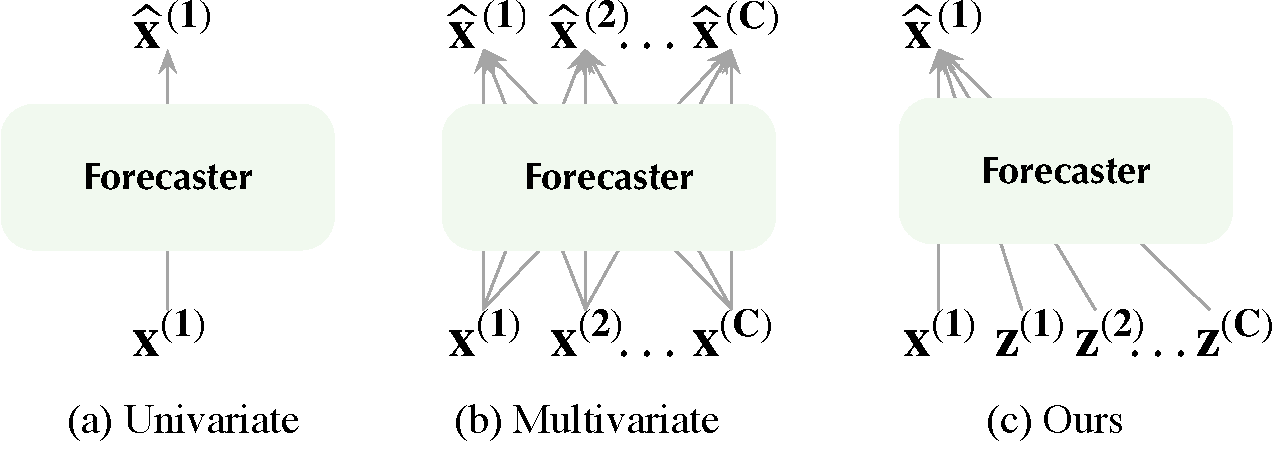
\includegraphics[width=\linewidth]{fig/Backgroundv4.pdf}
    \vspace{-20pt}
    \caption{Comparison between different forecasting paradigms. The inputs of forecasting with exogenous variables include multiple external variates $\{\mathbf{z}^{(1)},\cdots,\mathbf{z}^{(C)}\}$, which serve as auxiliary information and are not required for forecasting. }
    \label{fig:Compare-Forecasting}
    \vspace{-15pt}
\end{figure}

Time series forecasting is of pressing demand in real-world scenarios and can be widely used in various domains, such as weather \cite{wu2023interpretable, zhang2023skilful}, electricity market \cite{weron2014electricity}, and transportation \cite{lv2014traffic}. As shown in Figure \ref{fig:Compare-Forecasting}, existing forecasting paradigms can be summarized into three distant categories. In comparison with univariate and multivariate forecasting, forecasting with exogenous variables introduces auxiliary information to facilitate the forecasting of the endogenous variable. Exogenous variables are prevalent and indispensable in practical applications since the variations within time series data are often influenced by external factors, 
such as economic indicators, demographic changes, and societal events. For instance, electricity prices are highly dependent on the supply and demand of the market, and it is virtually impossible to predict future prices solely based on historical data. Incorporating external factors allows for a more comprehensive understanding of the interrelationships and causality among various variables, leading to better and more reliable performance, as well as interpretability.

Unlike previous well-established settings, since only the endogenous variable is of interest, forecasting with exogenous variables poses unique challenges. First, time series are often affected by multiple factors, which requires models to reconcile discrepancy and dependency among the \emph{endogenous} and \emph{exogenous} variables. 
Regarding exogenous variables equally with endogenous ones will not only cause significant time and memory complexity but also involve unnecessary interaction from endogenous series to external information. 
Second, the effects of external factors on endogenous series could be continuous and time-lagged.
Time series in real-world scenarios are often irregular, and exogenous variables may encounter problems such as missing data, misaligned lengths, and misaligned sampling times.

Given the crucial role of exogenous variables in time series forecasting, classical statistical models have already included exogenous variables as part of inputs, distinguishing them from endogenous ones. Despite the success of deep models in capturing intricate temporal dependencies in time series data, there are few models that support external input. Existing exogenous works usually struggle to capture complex long-term temporal dependencies \cite{olivares2023neural}. Transformers \cite{vaswani2017attention} have exhibited remarkable performance in time series forecasting thanks to their ability to capture both temporal dependencies and multivariate correlations. However, existing Transformer-based forecasters are not originally designed for forecasting with exogenous variables. 
Represented by PatchTST \cite{nie2022time}, existing variate-independent models are only capable of capturing temporal dependencies but fail to capture multivariate correlations.
Conversely, iTransformer \cite{liu2023itransformer} succeeds in capturing interrelationships between variables by using attention mechanisms on variate tokens but is unable to capture temporal variation between different sub-series since the whole series is embedded to a variate token by a temporal linear projection.

Beyond complicated designs, we discover that it is possible to make the canonical Transformers seamlessly adapt to exogenous variables without modifying the component or architecture. Specifically, in this paper, we excavate the potential of Transformer architecture and propose a \textbf{Time} Series Transform\textbf{er} with e\textbf{X}ogenous variables (\textbf{TimeXer}). By utilizing the series-level representation of time series data, TimeXer can capture correlations between multiple exogenous and endogenous variables through cross-attention. Since capturing the temporal dependencies within the endogenous series is indispensable for accurate prediction, TimeXer also includes patch-wise representations for endogenous series. This design allows TimeXer to capture the endogenous temporal dependencies using self-attention. Besides, the endogenous variate token effectively diffuses the external information to corresponding endogenous temporal patches. Extensive experiments demonstrate that TimeXer achieves state-of-the-art performance on various real-world datasets. Our contributions are summarized as:
\vspace{-5pt}
\begin{itemize}
    \item Motivated by the universality and importance of exogenous variables in time series forecasting, we empower the Transformer architecture to the inclusion of exogenous variables without architectural modifications.
    \item We propose TimeXer that utilizes different levels of representations of endogenous and exogenous variables to capture temporal dependencies by self-attention over patch-level endogenous temporal tokens and multivariate correlations by cross-attention over variate tokens.
    \item Extensive experiments on real-world datasets reveal that TimeXer can better utilize exogenous information to facilitate prediction than other forecasting models.
\end{itemize}


\section{Related Works}
\paragraph{Time Series Forecasting Models}
In recent years, deep models have achieved great progress in the field of time series analysis. Among all downstream tasks, time series forecasting is an essential problem where a large volume of work has been proposed to handle the intricate temporal dependencies, which can be divided into four categories: RNN-based, CNN-based, MLP-based, and Transformer-based models. RNN-based models, including LSTNet \cite{lai2018modeling} and DeepAR \cite{salinas2020deepar}, are suited for handling sequential temporal data, while they are restricted by gradient vanishing and inefficiency problems. With the power of convolutional kernels, recent works, such as TimesNet \cite{wu2023timesnet}, SCINet \cite{liu2022scinet} empower CNN in time series modeling and achieve comparable performance with a Transformer-based model.
Recently, MLP-based models led by N-BEATS \cite{oreshkin2019n} and DLinear \cite{zeng2023transformers} have emerged as competitive forecasters in the time series community. 

Motivated by the great success in the field of natural language processing \cite{devlin2018bert} and computer vision \cite{liu2021swin}, Transformers have garnered significant interest in time series data due to their ability to capture long-term temporal dependencies and complex multivariate correlations. Categorized based on the granularity of representation learning, Transformer-based models can be divided into point-wise, patch-wise, and series-wise as shown in Figure \ref{fig:Related-Work}. Due to the serial nature of time series, most previous works use a point-wise representation of time series data and apply attention mechanisms to capture the correlations among different time points. Therefore, many efficient Transformers \cite{zhou2021informer, wu2021autoformer, liu2021pyraformer, zhou2022fedformer} were proposed to reduce the complexity caused by point-wise modeling. Informer \cite{zhou2021informer} designs a ProbSparse self-attention to reduce the quadratic complexity in time and memory. Autoformer \cite{wu2021autoformer} replaces canoical self-attention with Auto-correlation to discover the sub-series similarity within time series data. Pyraformer \cite{liu2021pyraformer} develops a pyramidal attention module to capture both short- and long-temporal dependencies with linear time and space complexity. Considering point-wise representations fall short in revealing local semantic information lies in the temporal variation, PatchTST \cite{nie2022time} split time series data into subseries-level patches and then capture dependencies between patches.
Beyond capturing the patch-level temporal dependencies within one single series, recent approaches have endeavored to capture interdependencies among patches from different variables over time. Crossformer \cite{zhang2022crossformer} introduces a Two-Stage Attention layer to efficiently capture the cross-time and cross-variate dependencies of each patch. 
Further expanding the receptive field, iTransformer utilizes the global representation of the whole series and applies attention to these series-wise representations to capture multivariate correlations.
Yet, most of these methods only focus on multivariate or univariate time series forecasting and do not conduct special designs for exogenous variables, which is different from our setting in this paper.

\begin{figure}[t]
    \centering
    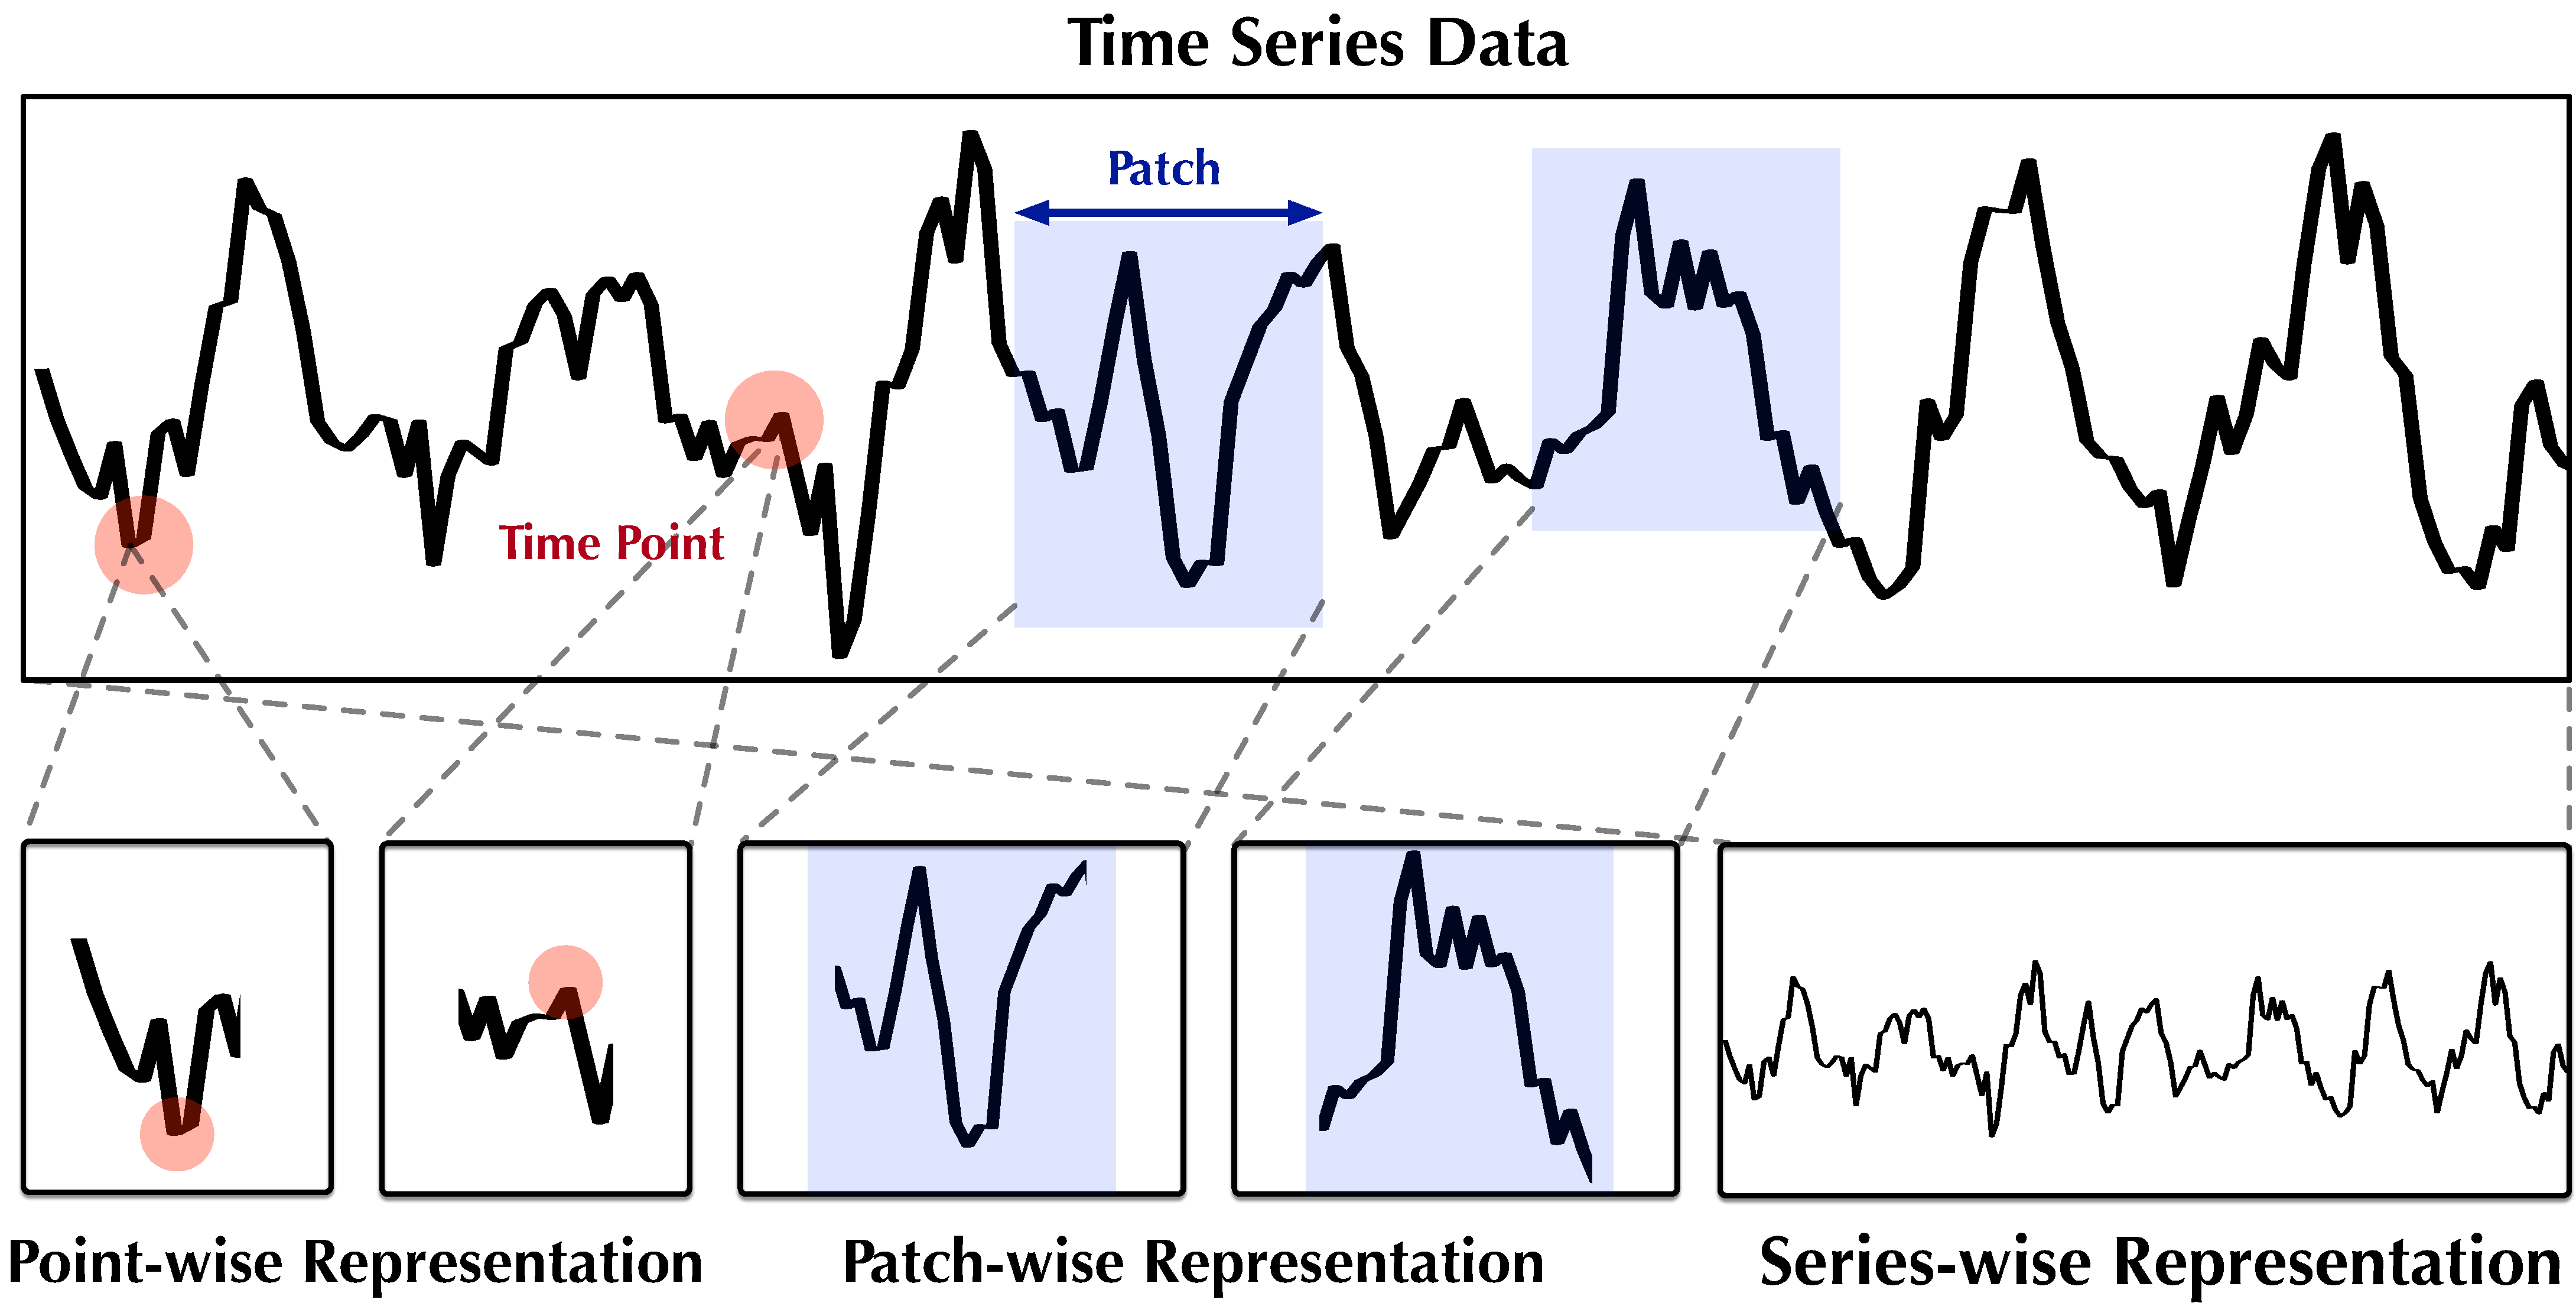
\includegraphics[width=\linewidth]{fig/Representationv5.pdf}
    \vspace{-15pt}
    \caption{Illustration of different levels of representation for time series data, ranging from point-wise, patch-wise to series-wise.}
    \vspace{-10pt}
    \label{fig:Related-Work}
\end{figure}

\vspace{-5pt}
\paragraph{Forecasting with Exogenous Variables}
Time series forecasting with exogenous variables has been widely discussed in classical statistical methods.
A vast majority of statistical methods have been extended to include exogenous variables as part of input.
Extending the acknowledged ARIMA model, ARIMAX \cite{williams2001multivariate} and SARIMAX \cite{vagropoulos2016comparison} incorporate the correlations between exogenous and endogenous variables along with the auto-regression on endogenous variables. Although time series modeling methods have evolved from statistical to deep models, most of the existing deep models incorporating covariates, such as Temporal Fusion Transformer (TFT) \cite{lim2021temporal}, primarily focus on variable selection. Some approaches, including NBEATSx \cite{olivares2023neural} and TiDE \cite{das2023long} contend that forecasting models are capable of accessing future values of exogenous variables during the prediction of endogenous variables. It is notable that previous models concatenate exogenous features with endogenous features at each time point and then map them to a latent space, necessitating the alignment of the endogenous and exogenous series in time. However, time series in real-world applications often suffer from problems such as missing value and uneven sampling, which leads to significant challenges in modeling the effects of exogenous variables on endogenous variables. In contrast, TimeXer introduces external information to Transformer architecture through a deftly designed embedding strategy, which can effectively introduce the external information into patch-wise representations of endogenous variables, thereby being enable to adapt to time-lagged or data-missing records.


\section{TimeXer}
In time series forecasting with exogenous variables, the endogenous time series represents the values to be predicted, while the exogenous variables are additional factors that may impact the endogenous series.

\paragraph{Problem Definition} Given an endogenous time series $ \mathbf{x}_{1:L} = \{x_1, x_2, ..., x_L\} \in \mathbb{R}^{L\times 1}$ and corresponding exogenous series $\mathbf{z}_{1:L'}=\{\mathbf{z}^{(1)}_{1:L'}, \mathbf{z}^{(2)}_{1:L'}, ..., \mathbf{z}^{(C)}_{1:L'}\} \in \mathbb{R}^{L\times C}$, where $L$ is the length of the look-back window of the endogenous variable, $x_i$ denotes the value at the $i$-th time points, $L'$ is the length of the look-back window of exogenous variables, $C$ is the number of exogenous variables, and $\mathbf{z}^{(i)}_{1:L'}$ represents the $i$-th exogenous variable. Note that the length of endogenous series $L$ and exogenous series $L'$ can be different.
The goal of forecasting model $f$ is to predict the future $S$ time steps  $\widehat{\mathbf{x}}=\{x_{L+1}, x_{L+2}, ..., x_{L+S}\}$ based on both historical observations $\mathbf{x}_{1:L}$ and corresponding exogenous series $\mathbf{z}_{1:L'}$, which can be formulated as follows:
\begin{equation}
    \mathbf{\widehat{x}} = f \left( \mathbf{x}_{1:L}, \mathbf{z}_{1:L'} \right).
\end{equation}

\begin{figure*}[h]
    \centering
   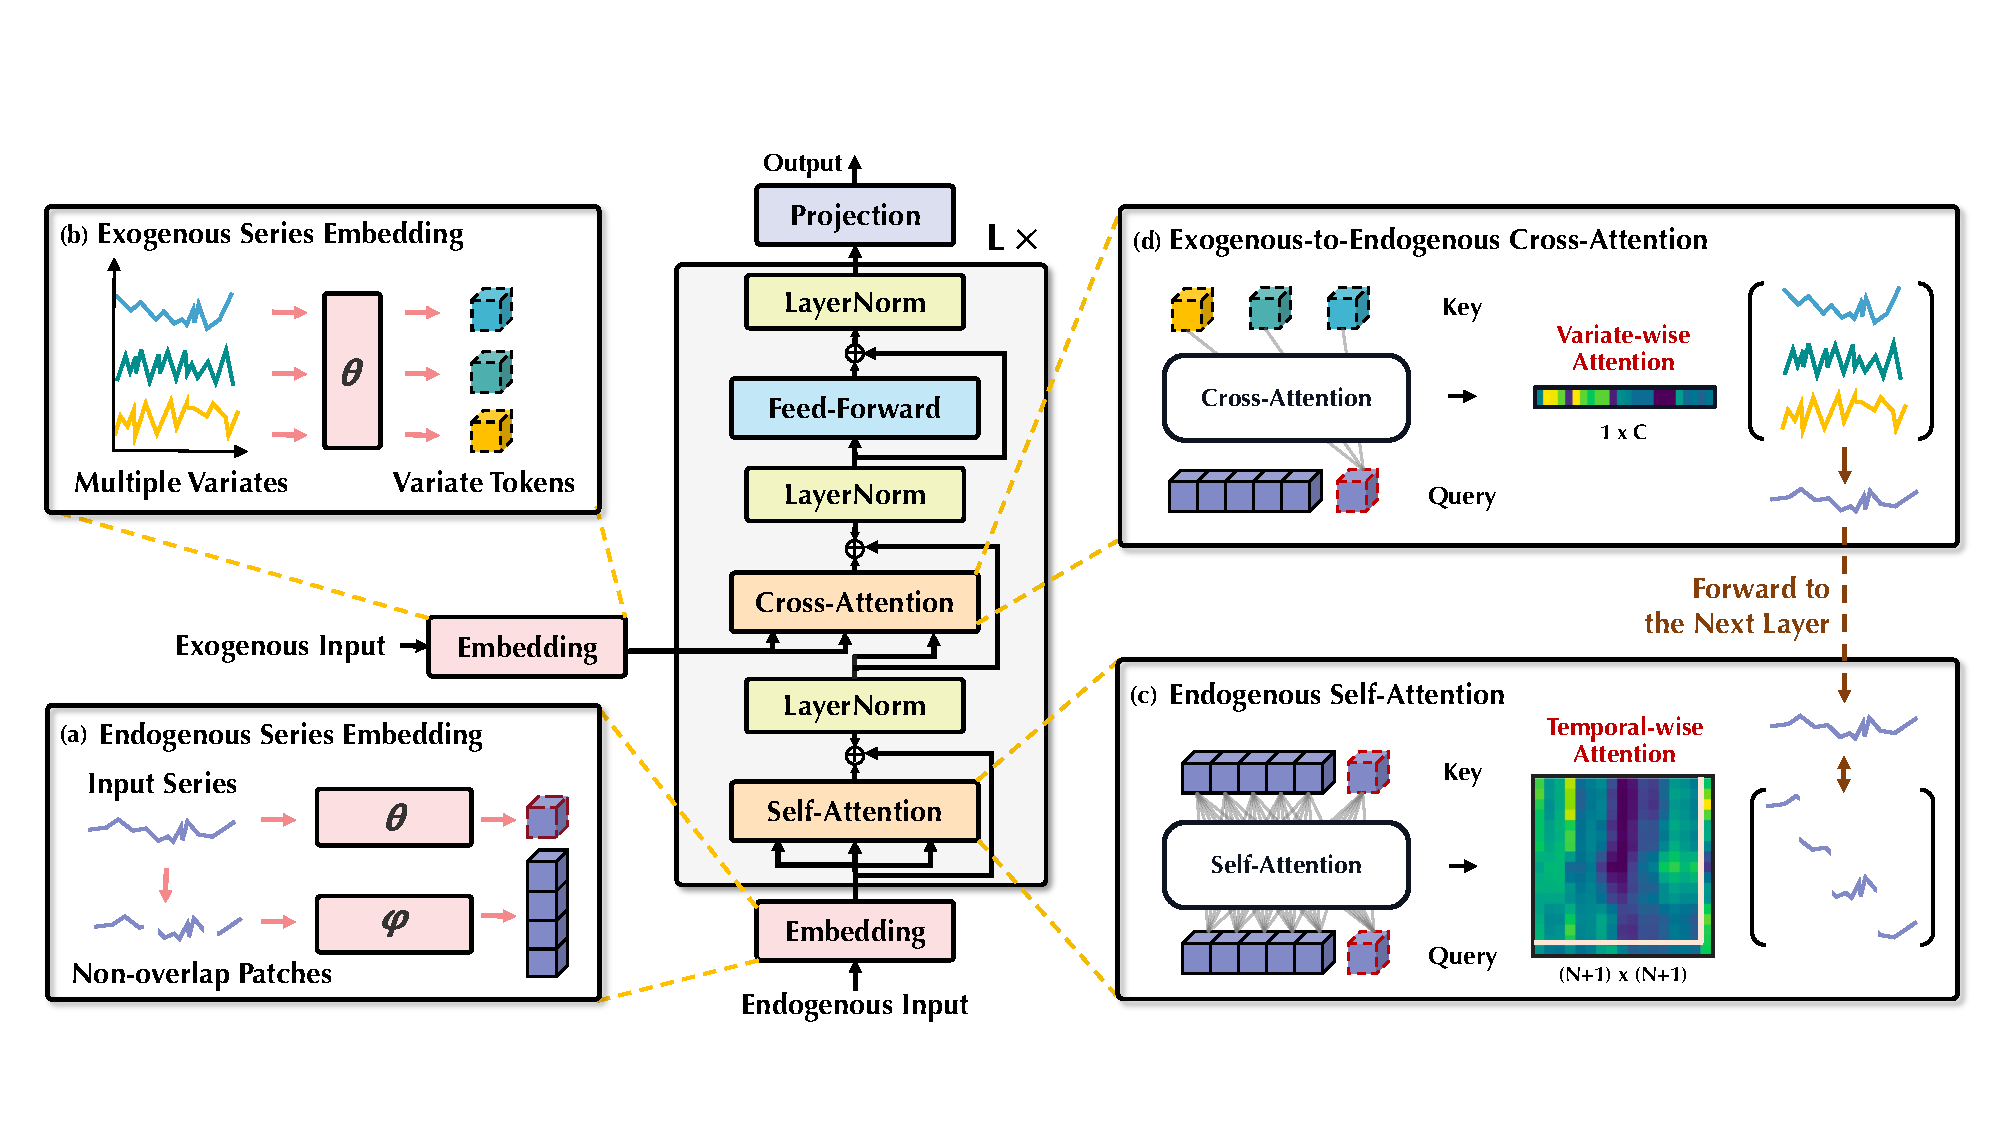
\includegraphics[width=0.98\linewidth]{fig/TimeXer.pdf}
    \label{fig:structure}
    \vspace{-5pt}
    \caption{The overall structure of TimeXer. TimeXer empowers the canonical Transformer to the processing of exogenous variables. (a) Both patch embedding and variate embedding are utilized for the endogenous variables to obtain multiple temporal tokens and a variate token respectively. (b) Each exogenous variable is embedded as a variate token through variate embedding. (c) Self-attention is applied to the endogenous temporal tokens to capture patch-wise dependencies. (d) Cross-attention is adopted to model the series-level dependencies over endogenous and exogenous variables.}
    \vspace{-10pt}
\end{figure*}

\vspace{-10pt}
\paragraph{Structure Overview}
As shown in Figure \ref{fig:structure}, our proposed TimeXer repurposes canonical Transformer without modifying any component, where variate embedding and patch embedding are introduced to address the difference between exogenous and endogenous variables. TimeXer adopts vanilla self-attention and cross-attention to capture temporal-wise and variate-wise dependencies respectively. 

\paragraph{Variate Embedding}
Most of the existing Transformer-based forecasting models embed each time point or a sub-series of time series data as a temporal token and apply self-attention to learn the temporal dependencies. Recent work \cite{liu2023itransformer} attempts to tokenize the whole time series as a variate token and adopt Transformer architecture to capture multivariate correlation. It is notable that in time series forecasting with exogenous variables, the model facilitates the prediction of the endogenous variable by capturing the correlations between endogenous and exogenous variables. Thus using too fine-grained representations of exogenous variables not only introduces significant computational complexity but also may introduce unnecessary noises due to, for instance, time misalignment.
Therefore, we utilize the series-global representation of both endogenous and exogenous series to model mutual interactions between different variables. Technically, TimeXer adopts a variate embedding to embed each series into a variate token, which can be summarized as follows: 
\begin{equation}
    \begin{aligned}
        \mathbf{V}_{en} &= \operatorname{EnVariateEmbed} \left(\mathbf{x}\right), \\
        \mathbf{V}_{ex,i} &= \operatorname{ExVariateEmbed} \big(\mathbf{z}^{(i)}\big)\ \text{$i\in\{1,\cdots, C\}$}.
    \end{aligned}
\end{equation}
The two variate-embedding layers $\operatorname{EnVariateEmbed}: \mathbb{R}^L \to \mathbb{R}^D$ and $\operatorname{ExVariateEmbed}: \mathbb{R}^{L^\prime} \to \mathbb{R}^D$ are instantiated as trainable linear projectors, where $L$ and $L^\prime$ are the look-back length of endogenous and exogenous series respectively. In this way, the embedded vector contains information of the whole series. $\mathbf{V}_{ex}=\{\mathbf{V}_{ex,i}\}_{i=1}^{C}$ denotes the set of representations for multiple exogenous series.


\paragraph{Patch Embedding}
Simultaneously, since the temporal causality is crucial for the forecast of the endogenous variable, we include the patch-wise representation to finely model the endogenous variable. Concretely, the endogenous series is split into non-overlap patches and each patch is projected to a temporal token. The patch embedding of the endogenous variable can be formulated as:
\begin{equation}
    \begin{aligned}
        \{\mathbf{s}_1, \mathbf{s}_2, ..., \mathbf{s}_N\} &= \operatorname{Patchify} \left(\mathbf{x}\right), \\
        \mathbf{P}_{en} &= \operatorname{PatchEmbed} \left(\mathbf{s}_1, \mathbf{s}_2, ..., \mathbf{s}_N\right). \\
    \end{aligned}
\end{equation}
Denote the patch length as $P$, $N = \lfloor \frac{L}{P} \rfloor$ is the number of patches of the endogenous series, and $\mathbf{s}_i$ denotes the $i$-th patch in the patch sequence. The $\operatorname{PatchEmbed}()$ map each patch of length $P$ into $D$ dimensions with a trainable linear projection and position embedding. In this way, the patch embedding of the endogenous variable $\mathbf{P}_{en} \in \mathbb{R}^{N \times D}$ contains $N$ patch-wise temporal tokens of $D$ dimension.
%The embedding result of endogenous variable $\mathbf{H}_{en} \in \mathbb{R}^{(N+1)\times D}$ is the concatenation of temporal-wise patch embedding $\mathbf{H}^t \in \mathbb{R}^{N\times D}$ and variate-wise embedding $\mathbf{H}^{v} \in \mathbb{R}^{1\times D}$.

\paragraph{Patch-wise Self-Attention}
In time series forecasting, it is essential for the model to capture the intrinsic temporal dependencies within the endogenous variable. Considering the exogenous variables that do not need to be predicted by the model, TimeXer applies attention to all endogenous tokens.
Concretely, the embedded vector of endogenous variables contains multiple patch-wise temporal tokens $\mathbf{\widehat P}_{en}$ and a series-wise variate token $\mathbf{\widehat V}_{en}$, where the variate token serves as a global token of the whole series, incorporating information from other temporal tokens. This provides a comprehensive view of the temporal dependencies within the endogenous variable, as well as better interaction with the series-wise variate tokens of the exogenous variables. The process can be formalized as:
\begin{equation}
    \mathbf{\widehat P}^l_{en}, \mathbf{\widehat V}^l_{en} = \operatorname{LN} \Big(\left[\mathbf{P}^l_{en}, \mathbf{V}^l_{en}\right] + \operatorname{Self-Attn}\left(\left[\mathbf{P}^l_{en}, \mathbf{V}^l_{en}\right]\right)\Big),
\end{equation}
where $l \in \{0,\cdots, M-1\}$ denotes the $l$-th TimeXer block.  $\mathbf{P}^l_{en}$ and $\mathbf{V}^l_{en}$ are the patch-wise and variate-wise token of the endogenous variable respectively, where $\mathbf{P}^0_{en}, \mathbf{V}^0_{en}$ are the embedded $\mathbf{P}_{en}, \mathbf{V}_{en}$. Here, $\left[ \cdot,\cdot\right]$ denotes the concatenation of the patch-wise and series-wise tokens of the endogenous variable along the sequence dimension. $\operatorname{Self-Attn}(\cdot)$ denotes the Multi-head Self-Attention over the endogenous tokens. $\operatorname{LN} (\cdot)$ denotes Layer Normalization.

\paragraph{Variate-wise Cross-Attention} Cross-attention has been widely used in multi-modal learning \cite{li2021align} to extract the dependencies between two different embedding vectors. In TimeXer, the cross-attention layer takes the endogenous variable as query and the exogenous variable as key and value to build the connection between the two types of variables. Since the exogenous variables are embedded as series-level variate tokens and are processed by the self-attention layer, we use the variate token of the endogenous variable to integrate information from exogenous variables. Then the output of cross-attention layers is then concatenated with the other endogenous temporal tokens. The above process can be formalized as:
\begin{equation}
    \begin{aligned}
        \mathbf{V}^{l+1}_{en} &= \operatorname{LN}\left(\mathbf{\widehat{V}}^{l}_{en} + \operatorname{Cross-Attn}\big(\mathbf{\widehat{V}}^{l}_{en}, \mathbf{V}_{ex}, \mathbf{V}_{ex}\big)\right).
    \end{aligned}
\end{equation}

Here, $\operatorname{Cross-Attn} (\cdot)$ denotes the Multi-head Cross-Attention between the endogenous and exogenous variables, where the query $\mathbf{\widehat{V}}^{l}_{en}$ is the endogenous variate token from the $l$-th TimeXer block, keys and values are the exogenous variate token $\mathbf{V}^{l}_{ex}$.
The output of the cross-attention layer $\mathbf{\widehat{V}}^{l}_{en}$  will become the input of the next self-attention layer. In this way, the multivariate correlations learned by the endogenous variate token can be further diffused to the endogenous temporal tokens, realizing the information transfer between exogenous variate tokens and endogenous temporal tokens.



\textbf{Forecasting Loss} As aforementioned in the problem definition, since the exogenous variables do not need to be predicted by the model, we apply a linear projection to the decoder output to yield the prediction of endogenous variables. Finally, we opt to use the L2 loss to measure the discrepancy between the prediction and the ground truth:
\begin{equation}
    \begin{aligned}
        \mathbf{\widehat{x}} &= {\rm{Projection}}(\mathbf{V}^{L}_{en}), \\
        \rm{Loss} &= \sum_{i=1}^{S}\|\mathbf{x}_{i}-\widehat{\mathbf{x}}_{i}\|_{2}^{2}.
    \end{aligned}
\end{equation}
where $L$ is the number of TimeXer block, $\mathbf{\widehat{x}} \in \mathbb{R}^{S\times 1}$ is the prediction of  future $S$ time steps of the endogenous variable.


\section{Experiments}
To verify the model's effectiveness, we extensively evaluate our proposed TimeXer on a diverse range of real-world time series datasets from different domains.


\paragraph{Datasets} To completely evaluate the forecasting capability of our proposed TimeXer, we conduct both short-term forecasting and long-term forecasting settings. For short-term forecasting tasks, we consider Electricity Price short-term Forecasting datasets (EPF) \cite{lago2021forecasting}, which is a real-world forecasting benchmark derived from five major power market data spanning six years each. Each dataset contains electricity price as an endogenous variable and two influential exogenous variables in practice. As for long-term forecasting, we adopt seven well-established public long-term multivariate forecasting benchmarks to perform forecasting with exogenous variables. We summarize the domain information of endogenous and exogenous variables for each dataset in Table \ref{tab:dataset}.

\begin{table}[h]
\renewcommand{\arraystretch}{1.5}
\vspace{-10pt}
\caption{Dataset descriptions. Note that the number of endogenous variables is 1 for all datasets, corresponding to multiple exogenous variables. Detailed descriptions are listed in the Appendix \ref{tab:full-dataset}.}
\vspace{5pt}
\begin{sc}
\centering
\resizebox{\linewidth}{!}{
\begin{tabular}{cccc}
\toprule[1.2pt]
\scalebox{1.35}{Dataset} & \scalebox{1.35}{Exogenous}   & \scalebox{1.35}{Endogenous} & \scalebox{1.35}{\#Num}  \\ \toprule[1.2pt]
\scalebox{1.35}{Electricity}    & \scalebox{1.35}{Electricity}         & \scalebox{1.35}{Electricity}  &  \scalebox{1.35}{320}       \\ \midrule
\scalebox{1.35}{Weather}    & \scalebox{1.35}{Climate}          & \scalebox{1.35}{Climate} & \scalebox{1.35}{20}     \\ \midrule
\scalebox{1.35}{ETTh}        & \scalebox{1.35}{Energy} & \scalebox{1.35}{Temperature}  & \scalebox{1.35}{6}   \\ \midrule
\scalebox{1.35}{ETTm}    & \scalebox{1.35}{Energy}   & \scalebox{1.35}{Temperature}  & \scalebox{1.35}{6}     \\ \midrule
\scalebox{1.35}{Traffic}   & \scalebox{1.35}{Transportation}  & \scalebox{1.35}{Transportation}  & \scalebox{1.35}{820}      \\ \midrule
\scalebox{1.35}{NP}& \scalebox{1.35}{Energy}                            & \scalebox{1.35}{Price}  & \scalebox{1.35}{2}            \\ \midrule
\scalebox{1.35}{PJM}     & \scalebox{1.35}{Energy}  & \scalebox{1.35}{Price}  & \scalebox{1.35}{2}  \\ \midrule
\scalebox{1.35}{BE}     & \scalebox{1.35}{Energy}  & \scalebox{1.35}{Price}  & \scalebox{1.35}{2}  \\ \midrule
\scalebox{1.35}{FR} & \scalebox{1.35}{Energy} & \scalebox{1.35}{Price}   & \scalebox{1.35}{2}   \\ \midrule
\scalebox{1.35}{DE}  & \scalebox{1.35}{Energy}   & \scalebox{1.35}{Price}   & \scalebox{1.35}{2}        \\ \bottomrule[1.2pt]
\end{tabular}}
\label{tab:dataset}
\end{sc}
\vspace{-10pt}
\end{table}



\paragraph{Baselines} We include 10 state-of-the-art deep forecasting models as our baselines, including Transformer-based model: iTransformer \cite{liu2023itransformer}, PatchTST \cite{nie2022time}, Crossformer \cite{zhang2022crossformer}, Stationary \cite{liu2022non}, Autoformer \cite{wu2021autoformer}, CNN-based model: TimesNet \cite{wu2023timesnet}, SCINet \cite{liu2022scinet}, and Linear-based model: RLinear \cite{li2023revisiting}, DLiear \cite{zeng2023transformers}, TiDE \cite{das2023long}. Among these models, TiDE is an advanced recent forecaster elaborated for exogenous variables.

\paragraph{Implementation Details} 
For short-term forecasting on EPF datasets, we set the patch length to 24 and follow the standard protocol in short-term electricity price forecasting \cite{olivares2023neural}, where the input length and predict length are set to 168 and 24. For long-term forecasting datasets, we uniformly set the patch length to 16 and fix the length of the lookback series as 96 and the prediction length varies $\{96, 192, 336, 720\}$.  

\begin{table*}[t]
\vspace{-10pt}
\setlength{\tabcolsep}{1pt}
\renewcommand{\arraystretch}{1.5}
\caption{Full results of the short-term forecasting task on EPF dataset. We follow the standard protocol in short-term electricity price forecasting, where the input length and predict length are set to 168 and 24 respectively for all baselines. Avg means the average results from all five datasets. The character ``.'' in the Transformers indicates the name of *former.}
\vspace{5pt}
\begin{sc}
\resizebox{\linewidth}{!}{
\begin{tabular}{c|cc|cc|cc|cc|cc|cc|cc|cc|cc|cc|cc} 
\toprule[1.2pt]
\multirow{2}{*}{\scalebox{1.35}{Model}}   & \multicolumn{2}{c}{\scalebox{1.35}{\textbf{TimeXer}}} & \multicolumn{2}{c}{\scalebox{1.35}{iTrans.}} & \multicolumn{2}{c}{\scalebox{1.35}{RLinear}} & \multicolumn{2}{c}{\scalebox{1.35}{PatchTST}} & \multicolumn{2}{c}{\scalebox{1.35}{Cross.}} & \multicolumn{2}{c}{\scalebox{1.35}{TiDE}} & \multicolumn{2}{c}{\scalebox{1.35}{TimesNet}} & \multicolumn{2}{c}{\scalebox{1.35}{DLinear}} & \multicolumn{2}{c}{\scalebox{1.35}{SCINet}} & \multicolumn{2}{c}{\scalebox{1.35}{Stationary}} & \multicolumn{2}{c}{\scalebox{1.35}{Auto.}} \\ 
& \multicolumn{2}{c}{\scalebox{1.35}{\textbf{(Ours)}}} & \multicolumn{2}{c}{\scalebox{1.35}{\citeyearpar{liu2023itransformer}}} & \multicolumn{2}{c}{\scalebox{1.35}{\citeyearpar{li2023revisiting}}} & \multicolumn{2}{c}{\scalebox{1.35}{\citeyearpar{nie2022time}}} & \multicolumn{2}{c}{\scalebox{1.35}{\citeyearpar{zhang2022crossformer}}} & \multicolumn{2}{c}{\scalebox{1.35}{\citeyearpar{das2023long}}} & \multicolumn{2}{c}{\scalebox{1.35}{\citeyearpar{wu2023timesnet}}} & \multicolumn{2}{c}{\scalebox{1.35}{\citeyearpar{zeng2023transformers}}} & \multicolumn{2}{c}{\scalebox{1.35}{\citeyearpar{liu2022scinet}}} & \multicolumn{2}{c}{\scalebox{1.35}{\citeyearpar{liu2022non}}} & \multicolumn{2}{c}{\scalebox{1.35}{\citeyearpar{wu2021autoformer}}} \\ 
\cmidrule(lr){2-3}\cmidrule(lr){4-5}\cmidrule(lr){6-7}\cmidrule(lr){8-9}\cmidrule(lr){10-11}\cmidrule(lr){12-13}\cmidrule(lr){14-15}\cmidrule(lr){16-17}\cmidrule(lr){18-19}\cmidrule(lr){20-21}\cmidrule(lr){22-23}
\scalebox{1.35}{Metric} & \scalebox{1.35}{MSE} & \scalebox{1.35}{MAE} & \scalebox{1.35}{MSE}    & \scalebox{1.35}{MAE}   & \scalebox{1.35}{MSE}    & \scalebox{1.35}{MAE}    & \scalebox{1.35}{MSE}    & \scalebox{1.35}{MAE} & \scalebox{1.35}{MSE}    & \scalebox{1.35}{MAE} & \scalebox{1.35}{MSE}    & \scalebox{1.35}{MAE}  & \scalebox{1.35}{MSE} & \scalebox{1.35}{MAE}      & \scalebox{1.35}{MSE}    & \scalebox{1.35}{MAE}  & \scalebox{1.35}{MSE}    & \scalebox{1.35}{MAE} & \scalebox{1.35}{MSE}    & \scalebox{1.35}{MAE}     & \scalebox{1.35}{MSE} & \scalebox{1.35}{MAE}            \\ 
\toprule[1.2pt]
\scalebox{1.35}{NP}     & \scalebox{1.35}{\textbf{0.238}} &  \scalebox{1.35}{\textbf{0.268}}             
& \scalebox{1.35}{0.265} & \scalebox{1.35}{0.300}                  & \scalebox{1.35}{0.335} & \scalebox{1.35}{0.340}             &
\scalebox{1.35}{0.267} & \scalebox{1.35}{0.284}              & \scalebox{1.35}{0.245} & \scalebox{1.35}{0.289}                 & \scalebox{1.35}{0.335} & \scalebox{1.35}{0.340}          & \scalebox{1.35}{0.250} & \scalebox{1.35}{0.289}              & \scalebox{1.35}{0.309} & \scalebox{1.35}{0.321}             & \scalebox{1.35}{0.373} & \scalebox{1.35}{0.368}            & \scalebox{1.35}{0.294} & \scalebox{1.35}{0.308}                & \scalebox{1.35}{0.402} & \scalebox{1.35}{0.398}             \\ \midrule
\scalebox{1.35}{PJM}    & \scalebox{1.35}{\textbf{0.088}} & \scalebox{1.35}{\textbf{0.188}}    
& \scalebox{1.35}{0.097} & \scalebox{1.35}{0.197}     &    \scalebox{1.35}{0.124} & \scalebox{1.35}{0.229}        &   
\scalebox{1.35}{0.106} & \scalebox{1.35}{0.209}       &  
\scalebox{1.35}{0.149} & \scalebox{1.35}{0.198}       &          \scalebox{1.35}{0.124} & \scalebox{1.35}{0.228}    & \scalebox{1.35}{0.097} & \scalebox{1.35}{0.195}  & \scalebox{1.35}{0.108} & \scalebox{1.35}{0.215}             & \scalebox{1.35}{0.143} & \scalebox{1.35}{0.259}            & \scalebox{1.35}{0.122} & \scalebox{1.35}{0.228}                & \scalebox{1.35}{0.168} & \scalebox{1.35}{0.267}                 \\ \midrule
\scalebox{1.35}{BE}     & \scalebox{1.35}{\textbf{0.374}} & \scalebox{1.35}{\textbf{0.241}}   
& \scalebox{1.35}{0.394} & \scalebox{1.35}{0.270}  &       \scalebox{1.35}{0.520} & \scalebox{1.35}{0.337}             & 
\scalebox{1.35}{0.403} & \scalebox{1.35}{0.264}      &     
 \scalebox{1.35}{0.436} & \scalebox{1.35}{0.294}                 & \scalebox{1.35}{0.523} & \scalebox{1.35}{0.336}   & \scalebox{1.35}{0.419} & \scalebox{1.35}{0.288}    & \scalebox{1.35}{0.463} & \scalebox{1.35}{0.313}             & \scalebox{1.35}{0.731} & \scalebox{1.35}{0.412}   & \scalebox{1.35}{0.433} & \scalebox{1.35}{0.289}      & \scalebox{1.35}{0.500} & \scalebox{1.35}{0.333}                 \\ \midrule
\scalebox{1.35}{FR}     & \scalebox{1.35}{\textbf{0.381}} & \scalebox{1.35}{\textbf{0.211}}  & 
\scalebox{1.35}{0.439} & \scalebox{1.35}{0.233}    & 
\scalebox{1.35}{0.507} & \scalebox{1.35}{0.290}     &      
\scalebox{1.35}{0.411} & \scalebox{1.35}{0.220}  & 
\scalebox{1.35}{0.440} & \scalebox{1.35}{0.216}    & \scalebox{1.35}{0.510} & \scalebox{1.35}{0.290}   & \scalebox{1.35}{0.431} & \scalebox{1.35}{0.234}     & \scalebox{1.35}{0.429} & \scalebox{1.35}{0.260}   & \scalebox{1.35}{0.855} & \scalebox{1.35}{0.384}            & \scalebox{1.35}{0.466} & \scalebox{1.35}{0.242}       & \scalebox{1.35}{0.519} & \scalebox{1.35}{0.295}                 \\ \midrule
\scalebox{1.35}{DE}     & \scalebox{1.35}{\textbf{0.440}} & \scalebox{1.35}{\textbf{0.418}}  
& \scalebox{1.35}{0.479} & \scalebox{1.35}{0.443}    &     \scalebox{1.35}{0.574} & \scalebox{1.35}{0.498}       &    
\scalebox{1.35}{0.461} & \scalebox{1.35}{0.432}    &    
\scalebox{1.35}{0.540} & \scalebox{1.35}{0.423}      &     
\scalebox{1.35}{0.568} & \scalebox{1.35}{0.496}   & \scalebox{1.35}{0.502} & \scalebox{1.35}{0.446}     & \scalebox{1.35}{0.520} & \scalebox{1.35}{0.463}   & \scalebox{1.35}{0.565} & \scalebox{1.35}{0.497}  & \scalebox{1.35}{0.483} & \scalebox{1.35}{0.447}                & \scalebox{1.35}{0.674} & \scalebox{1.35}{0.544}      \\ \midrule
\scalebox{1.35}{AVG}    & \scalebox{1.35}{\textbf{0.304}} & \scalebox{1.35}{\textbf{0.265}}  & 
\scalebox{1.35}{0.335} & \scalebox{1.35}{0.289}     &      \scalebox{1.35}{0.412} & \scalebox{1.35}{0.339}  &  
\scalebox{1.35}{0.330} & \scalebox{1.35}{0.282} &          
\scalebox{1.35}{0.362} & \scalebox{1.35}{0.284}    & \scalebox{1.35}{0.412} & \scalebox{1.35}{0.338}     & \scalebox{1.35}{0.340} & \scalebox{1.35}{0.290}    & \scalebox{1.35}{0.366} & \scalebox{1.35}{0.314}   & \scalebox{1.35}{0.533} & \scalebox{1.35}{0.384}            & \scalebox{1.35}{0.360} & \scalebox{1.35}{0.303}                & \scalebox{1.35}{0.453} & \scalebox{1.35}{0.368}                 \\ 
\bottomrule[1.2pt]
\end{tabular}}
\end{sc}
\label{tab:epf-forecast}
\vspace{-5pt}
\end{table*}

\begin{table*}[h]
%\vspace{-5pt}
\setlength{\tabcolsep}{1pt}
\renewcommand{\arraystretch}{1.5}
\caption{Full results of the long-term forecasting with exogenous variables. We compare extensive competitive models under different prediction lengths following the setting of iTransformer \cite{liu2023itransformer}. The input sequence length is set to 96 for all baselines. Results are averaged from all prediction lengths. The character ``.'' in the Transformers indicates the name of *former. ``-'' denotes out of memory (OOM) problem. The complete results are listed in the Appendix \ref{tab:full-log}.}
\vspace{5pt}
\begin{sc}
\resizebox{\linewidth}{!}{
\begin{tabular}{c|cc|cc|cc|cc|cc|cc|cc|cc|cc|cc|cc} 
\toprule[1.2pt]
\multirow{2}{*}{\scalebox{1.35}{Model}}   & \multicolumn{2}{c}{\scalebox{1.35}{\textbf{TimeXer}}} & \multicolumn{2}{c}{\scalebox{1.35}{iTrans.}} & \multicolumn{2}{c}{\scalebox{1.35}{RLinear}} & \multicolumn{2}{c}{\scalebox{1.35}{PatchTST}} & \multicolumn{2}{c}{\scalebox{1.35}{Cross.}} & \multicolumn{2}{c}{\scalebox{1.35}{TiDE}} & \multicolumn{2}{c}{\scalebox{1.35}{TimesNet}} & \multicolumn{2}{c}{\scalebox{1.35}{DLinear}} & \multicolumn{2}{c}{\scalebox{1.35}{SCINet}} & \multicolumn{2}{c}{\scalebox{1.35}{Stationary}} & \multicolumn{2}{c}{\scalebox{1.35}{Auto.}} \\ 
& \multicolumn{2}{c}{\scalebox{1.35}{\textbf{(Ours)}}} & \multicolumn{2}{c}{\scalebox{1.35}{\citeyearpar{liu2023itransformer}}} & \multicolumn{2}{c}{\scalebox{1.35}{\citeyearpar{li2023revisiting}}} & \multicolumn{2}{c}{\scalebox{1.35}{\citeyearpar{nie2022time}}} & \multicolumn{2}{c}{\scalebox{1.35}{\citeyearpar{zhang2022crossformer}}} & \multicolumn{2}{c}{\scalebox{1.35}{\citeyearpar{das2023long}}} & \multicolumn{2}{c}{\scalebox{1.35}{\citeyearpar{wu2023timesnet}}} & \multicolumn{2}{c}{\scalebox{1.35}{\citeyearpar{zeng2023transformers}}} & \multicolumn{2}{c}{\scalebox{1.35}{\citeyearpar{liu2022scinet}}} & \multicolumn{2}{c}{\scalebox{1.35}{\citeyearpar{liu2022non}}} & \multicolumn{2}{c}{\scalebox{1.35}{\citeyearpar{wu2021autoformer}}} \\ 
\cmidrule(lr){2-3}\cmidrule(lr){4-5}\cmidrule(lr){6-7}\cmidrule(lr){8-9}\cmidrule(lr){10-11}\cmidrule(lr){12-13}\cmidrule(lr){14-15}\cmidrule(lr){16-17}\cmidrule(lr){18-19}\cmidrule(lr){20-21}\cmidrule(lr){22-23}
\scalebox{1.35}{Metric} & \scalebox{1.35}{MSE}          & \scalebox{1.35}{MAE}          & \scalebox{1.35}{MSE}             & \scalebox{1.35}{MAE}            & \scalebox{1.35}{MSE}           & \scalebox{1.35}{MAE}          & \scalebox{1.35}{MSE}          & \scalebox{1.35}{MAE}          & \scalebox{1.35}{MSE}            & \scalebox{1.35}{MAE}            & \scalebox{1.35}{MSE}         & \scalebox{1.35}{MAE}        & \scalebox{1.35}{MSE}           & \scalebox{1.35}{MAE}          & \scalebox{1.35}{MSE}          & \scalebox{1.35}{MAE}          & \scalebox{1.35}{MSE}          & \scalebox{1.35}{MAE}         & \scalebox{1.35}{MSE}            & \scalebox{1.35}{MAE}           & \scalebox{1.35}{MSE}            & \scalebox{1.35}{MAE}
\\ \toprule[1.2pt]
\scalebox{1.35}{ECL}     & {\scalebox{1.35}{\textbf{0.336}}}        & {\scalebox{1.35}{\textbf{0.414}}}        &  \scalebox{1.35}{0.365}           & \scalebox{1.35}{0.442}          & 
\scalebox{1.35}{0.444}        & \scalebox{1.35}{0.486} &
\scalebox{1.35}{0.394}         & \scalebox{1.35}{0.446}       & \scalebox{1.35}{0.344}          & \scalebox{1.35}{0.412}          & \scalebox{1.35}{0.419}       & \scalebox{1.35}{0.468}      & \scalebox{1.35}{0.410}         & \scalebox{1.35}{0.476}        & \scalebox{1.35}{0.393}        & \scalebox{1.35}{0.457}        &   \scalebox{1.35}{0.427}          &  	\scalebox{1.35}{0.490}          & \scalebox{1.35}{0.372}          & \scalebox{1.35}{0.450}         & \scalebox{1.35}{0.495}          & \scalebox{1.35}{0.528}         \\ \midrule
\scalebox{1.35}{Weather} & \scalebox{1.35}{0.002}        & \scalebox{1.35}{0.031}        & \scalebox{1.35}{0.002}           & \scalebox{1.35}{0.031}          & \scalebox{1.35}{\textbf{0.002}}         & \scalebox{1.35}{\textbf{0.029}}        & \scalebox{1.35}{0.002}        & \scalebox{1.35}{0.031}   & \scalebox{1.35}{0.005}          & \scalebox{1.35}{0.055}          & \scalebox{1.35}{\textbf{0.002}}       & \scalebox{1.35}{\textbf{0.029}}      & \scalebox{1.35}{0.097}         & \scalebox{1.35}{0.115}        & \scalebox{1.35}{0.006}        & \scalebox{1.35}{0.066}        &    \scalebox{1.35}{0.007}    &   	\scalebox{1.35}{0.071}           & \scalebox{1.35}{0.002}        & \scalebox{1.35}{0.031}         & \scalebox{1.35}{0.006}          & \scalebox{1.35}{0.060}  \\ \midrule
\scalebox{1.35}{ETTh1}   & \scalebox{1.35}{\textbf{0.074}}        & \scalebox{1.35}{\textbf{0.210}}        
& \scalebox{1.35}{0.075}           & \scalebox{1.35}{0.211}          & 
\scalebox{1.35}{0.084}        & \scalebox{1.35}{0.224}        & \scalebox{1.35}{0.078}         & \scalebox{1.35}{0.215}        & \scalebox{1.35}{0.285}          & \scalebox{1.35}{0.447}          & \scalebox{1.35}{0.083}       & \scalebox{1.35}{0.223}      & \scalebox{1.35}{0.076}         & \scalebox{1.35}{0.215}        & \scalebox{1.35}{0.116}        & \scalebox{1.35}{0.259}        &  \scalebox{1.35}{0.437}        & 	\scalebox{1.35}{0.565}             & \scalebox{1.35}{0.110}          & \scalebox{1.35}{0.256}         & \scalebox{1.35}{0.130}        & \scalebox{1.35}{0.282}    \\ \midrule
\scalebox{1.35}{ETTh2}   & \scalebox{1.35}{\textbf{0.183}}       & \scalebox{1.35}{\textbf{0.337}}   
& \scalebox{1.35}{0.199} & \scalebox{1.35}{0.352}          & \scalebox{1.35}{0.205}        & \scalebox{1.35}{0.356}        & 
\scalebox{1.35}{0.192}         & \scalebox{1.35}{0.345}        & \scalebox{1.35}{1.027}          & \scalebox{1.35}{0.873}          & \scalebox{1.35}{0.205}       & \scalebox{1.35}{0.356}      & \scalebox{1.35}{0.210}         & \scalebox{1.35}{0.362}        & \scalebox{1.35}{0.224}        & \scalebox{1.35}{0.369}        & \scalebox{1.35}{1.155}   &  
\scalebox{1.35}{0.955}      & \scalebox{1.35}{0.262}          & \scalebox{1.35}{0.405}         & \scalebox{1.35}{0.242}          & \scalebox{1.35}{0.386}         \\ \midrule
\scalebox{1.35}{ETTm1}   & \scalebox{1.35}{\textbf{0.051}}     &  \scalebox{1.35}{\textbf{0.169}}       
& \scalebox{1.35}{0.053}  & \scalebox{1.35}{0.175}   & 
\scalebox{1.35}{0.053}   & \scalebox{1.35}{0.173}   & 
\scalebox{1.35}{0.053}        & \scalebox{1.35}{0.173}        & \scalebox{1.35}{0.411}          & \scalebox{1.35}{0.548}  & 
\scalebox{1.35}{0.053}       & \scalebox{1.35}{0.173}      & \scalebox{1.35}{0.054}         & \scalebox{1.35}{0.175}        & \scalebox{1.35}{0.066}        & \scalebox{1.35}{0.188}        &  \scalebox{1.35}{0.098}     &   \scalebox{1.35}{0.241}     & 
\scalebox{1.35}{0.077}       & \scalebox{1.35}{0.204}      & \scalebox{1.35}{0.085}     & \scalebox{1.35}{0.230}         \\ \midrule
\scalebox{1.35}{ETTm2}   &  \scalebox{1.35}{\textbf{0.116}}        & \scalebox{1.35}{\textbf{0.252}}    &
\scalebox{1.35}{0.127}  & \scalebox{1.35}{0.267}        & 
\scalebox{1.35}{0.122}     &  \scalebox{1.35}{0.261}           & 
\scalebox{1.35}{0.120} & \scalebox{1.35}{0.258}        &  
\scalebox{1.35}{0.976}          & \scalebox{1.35}{0.769}          &   \scalebox{1.35}{0.122}   &  	\scalebox{1.35}{0.261}                & \scalebox{1.35}{0.129}         & \scalebox{1.35}{0.271}        & \scalebox{1.35}{0.126}        & \scalebox{1.35}{0.263}       &    \scalebox{1.35}{0.685} & \scalebox{1.35}{0.713}       & 
\scalebox{1.35}{0.207}   & \scalebox{1.35}{0.333}         & \scalebox{1.35}{0.154}          & \scalebox{1.35}{0.305}         \\ \midrule
\scalebox{1.35}{Traffic} &  \scalebox{1.35}{\textbf{0.150}}        &  \scalebox{1.35}{\textbf{0.227}}     
& \scalebox{1.35}{0.161}       & \scalebox{1.35}{0.246}     & \scalebox{1.35}{0.324}        & \scalebox{1.35}{0.412}        & 
\scalebox{1.35}{0.173}         & \scalebox{1.35}{0.253}        & 
\scalebox{1.35}{-}          & \scalebox{1.35}{-}          & \scalebox{1.35}{0.324}       & \scalebox{1.35}{0.411}      & \scalebox{1.35}{0.171}         & \scalebox{1.35}{0.264}        & \scalebox{1.35}{0.323}        & \scalebox{1.35}{0.404}        &  \scalebox{1.35}{0.447} 	&   \scalebox{1.35}{0.500}         & \scalebox{1.35}{0.361}          & \scalebox{1.35}{0.361}         & \scalebox{1.35}{0.302}          & \scalebox{1.35}{0.353}         \\ \bottomrule[1.2pt]
\end{tabular}}
\end{sc}
\label{tab:multi-result}
\vspace{-10pt}
\end{table*}




\subsection{Main Results}
Comprehensive short-term and long-term forecasting results are listed in Table \ref{tab:epf-forecast} and Table \ref{tab:multi-result}. A lower MSE or MAE indicates more accurate forecasting results.

Short-term Electricity Price Forecasting task is derived from real-world scenarios, and presents a unique challenge for the forecasting model for the endogenous variable have been shown to be highly correlated with two exogenous variables in the dataset. As shown in Table \ref{tab:epf-forecast}, TimeXer achieves consistent state-of-the-art performance on all five datasets, outperforming various baseline models. Notably, linear forecasters fail to triumph over Transformer-based forecasters in this task.
In contrast, with attention mechanisms, Transformer-based models are better equipped to capture relationships between intra-time and inter-time series data.
It is notable that for channel-independent models led by DLinear and PathTST, while they include exogenous variables as part of the input, they solely perform univariate forecasting on the endogenous variable. In contrast, TimeXer effectively integrates information from exogenous variables and surpasses the performance of univariate forecasting. Similar to TimeXer, Crossformer divides all input series into segments and captures multivariate correlations over all segments; however, it fails to outperform other baselines, suggesting that modeling all variables at a granular level introduces unnecessary noise into the forecasting. Conversely, iTransformer neglects the temporal-wise attention module, indicating that there are still limitations in capturing temporal dependencies solely through linear projection. Therefore, TimeXer strikes a balance between avoiding distractions caused by fine-grained modeling of exogenous variables and addressing inaccuracies resulting from coarse-grained temporal modeling of endogenous variables, ultimately achieving state-of-the-art performance.

We also evaluate the performance of TimeXer on established long-term forecasting benchmarks. Unlike short-term forecasts, which contain only two releated exogenous variables, the long-term multivariate dataset has a large number of exogenous variables, and not all exogenous variables are related to the endogenous variable.
As listed in Table \ref{tab:multi-result}, TimeXer shows great performance in the vast majority datasets, which demonstrates that TimeXer are effective in capturing beneficial information for forecasting.

\subsection{Abalation Studies}

\paragraph{Masking Exogenous Variables} Real-world time series encounter problems such as missing data that result in low-quality data. In this section, we use random masking to replicate these situations and further explore the forecasting performance when fed low-quality data. Previous works \cite{dong2023simmtm} have demonstrated that the semantic information of time series lies in temporal variation, We use complete, high-quality historical data for the endogenous variables and progressively reduce the quality of the data for the exogenous variables by increasing the masking ratio from 0\% (i.e., using complete historical data for the exogenous variables) to 99\%.
It can be observed that with the decrease in the quality of the exogenous series, the forecasting performance of the model also decreases. Notably, our model maintains a competitive performance when the exogenous series are masked by a small amount, which indicates that our proposed TimeXer is capable of supporting low-quality data scenarios.
\begin{figure}[h]
    \centering
    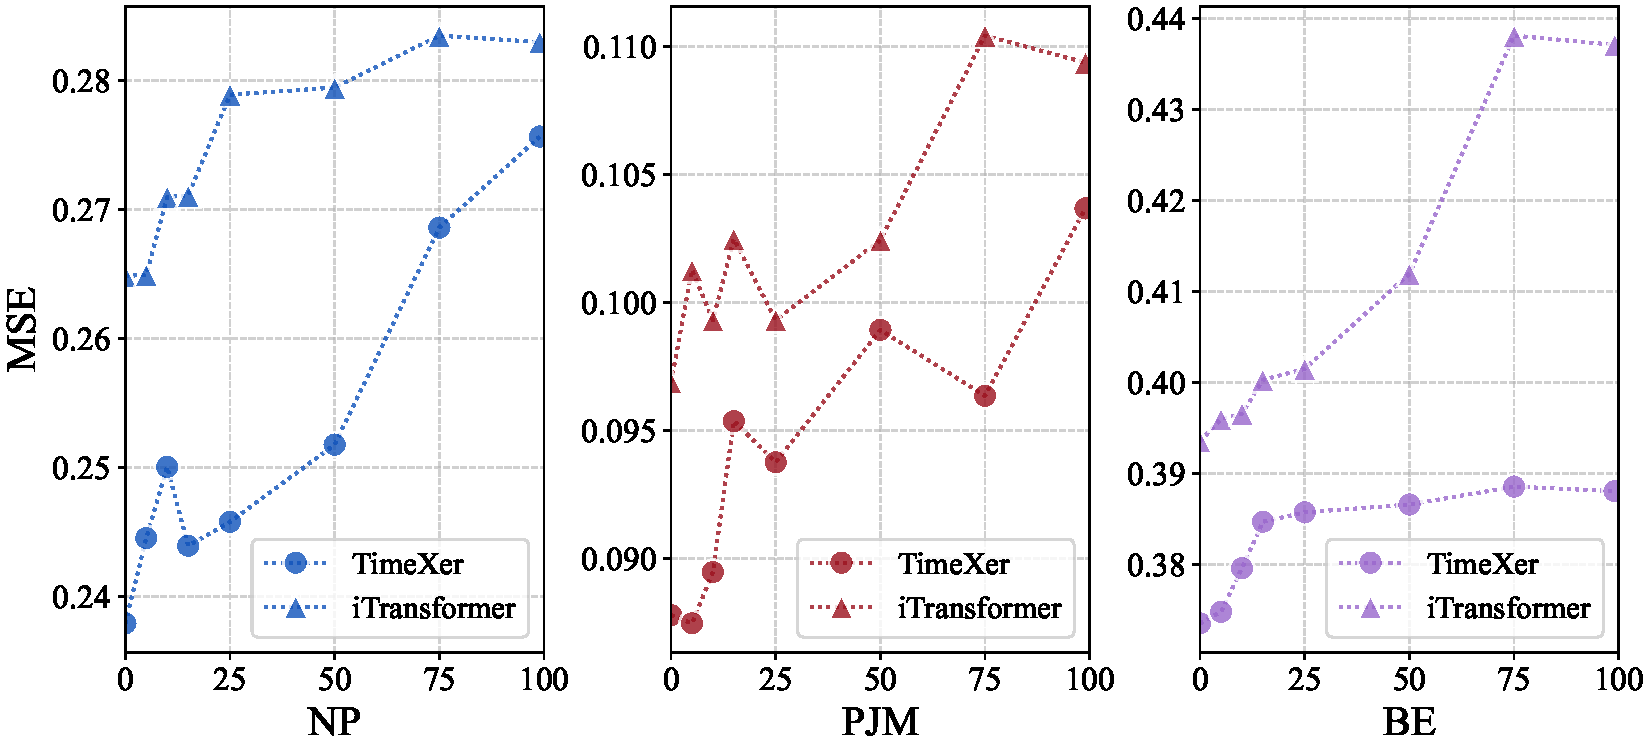
\includegraphics[width=\linewidth]{fig/maskv3.pdf}
    \vspace{-20pt}
    \caption{Forecasting performance with the masked exogenous series on three EPF datasets, simulating the missing data scenario.}
    \vspace{-10pt}
    \label{fig:mask}
\end{figure}


\paragraph{Varying Different Embeddings} In our TimeXer, we utilize inverted embedding to obtain series-level representations of exogenous and endogenous variables. Besides, patch embedding is utilized to get patch-level temporal representations of the endogenous variable.
To elaborate on the validity of our embedding strategy for endogenous and exogenous variables, we conducted detailed ablations. Specifically, for exogenous variables, we replace existing series-level representations with temporal-wise representations. For endogenous variables, we remove different components of the embedded vector. As shown in Table \ref{tab:abalation}, among various architectural designs, TimeXer exhibits superior performance across all datasets. Compared to the second design which replaces the variate token for each exogenous variable with multiple temporal tokens to capture interrelationships between the different variables, TimeXer achieves superior forecasting performance with lower complexity. Notably, the performance of the third and fourth designs indicates that for endogenous variables, both temporal and variate tokens are indispensable.

\begin{table}[h]
\centering
\vspace{-10pt}
\caption{Ablation Results. \emph{Ex.} and \emph{En.} are abbreviations for Exogenous variable and Endogenous variable. \emph{T} and \emph{V} denote temporal token and variate token respectively. Results are averaged from all prediction lengths. Full results are listed in the Appendix.}
\vspace{5pt}
\setlength{\tabcolsep}{2.5pt}
\renewcommand{\arraystretch}{1.2}
\begin{sc}
\resizebox{\linewidth}{!}{
\begin{tabular}{c|c|c|cc|cc|cc}
\toprule[1.2pt]
\multirow{2}{*}{Design} & \multirow{2}{*}{En.} & \multirow{2}{*}{Ex.} & \multicolumn{2}{c}{ETTh2} & \multicolumn{2}{c}{ETTm2} & \multicolumn{2}{c}{Traffic}  \\
\cmidrule(lr){4-5}\cmidrule(lr){6-7}\cmidrule(lr){8-9}
                        &                      &                      & MSE    & MAE              & MSE    & MAE                & MSE    & MAE             \\ \toprule[1.2pt]
\textbf{Ours}                    & T+V                  & V                    & {\textbf{0.183}} & {\textbf{0.337}}  &{\textbf{ 0.116}} &  {\textbf{0.252}}           & {\textbf{0.150}} & {\textbf{0.227}}       \\ \midrule
Replace                 & T+V                  & T                    &  0.192 & 0.343 & 0.122 & 0.259 &	0.158 &	0.239   \\ \midrule
\textbf{\multirow{2}{*}{w/o}}    & w/o V                & V                    & 0.197 & 0.347 & 0.117 & 0.254           & 0.158 & 0.239  \\ 
                        & w/o T                & V                    & 0.188 & 0.341 & 0.118 & 0.256           & 0.152 & 0.233       \\ \bottomrule[1.2pt]
\end{tabular}}
\end{sc}
\label{tab:abalation}
\end{table}


\subsection{Model Analysis}
\begin{figure}[h]
    \centering
    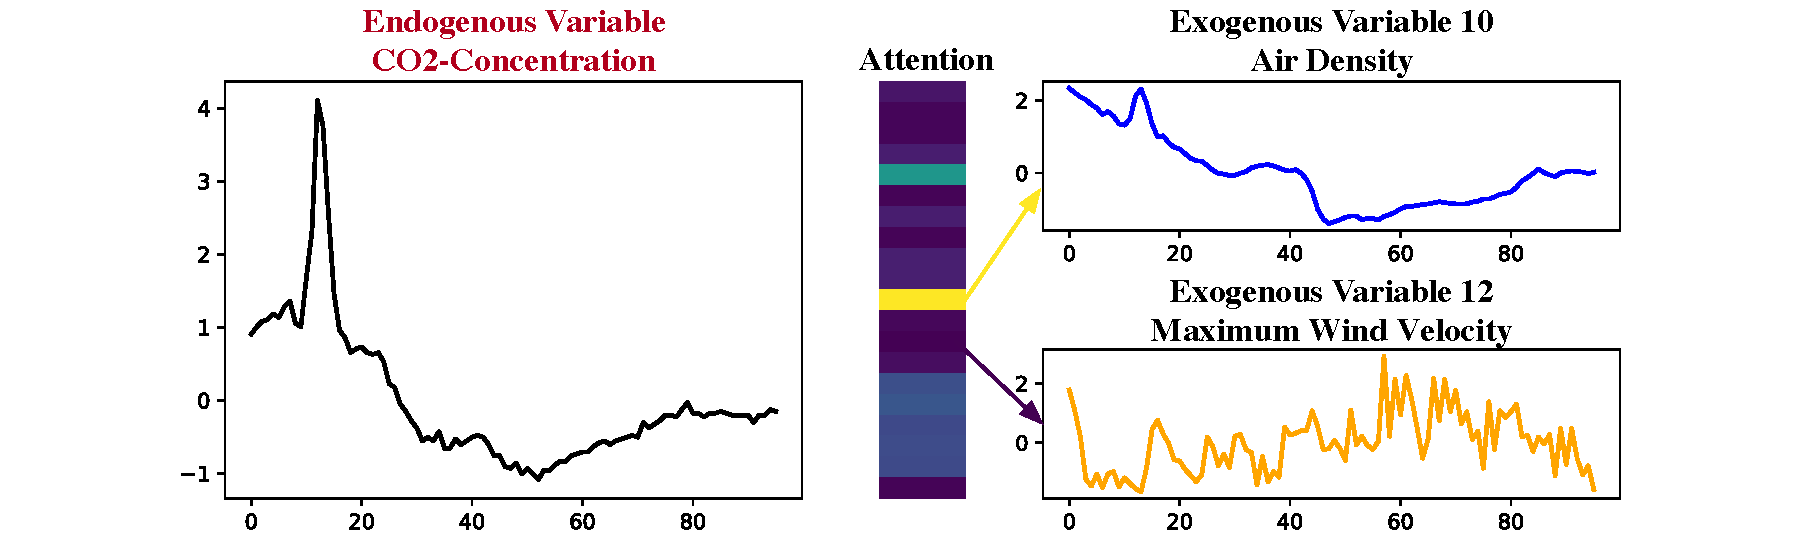
\includegraphics[width=\linewidth]{fig/visv3.pdf}
    \vspace{-10pt}
    \caption{Visualization of learned attention map alongside the endogenous time series and the exogenous time series with highest and lowest attention scores.}
    \vspace{-10pt}
    \label{fig:attn-vis}
\end{figure}
\paragraph{Analysis of Variate-wise Correlations}
TimeXer adopts cross-attention on series-wise variate tokens to capture the multivariate correlation between the endogenous and exogenous variables, enhancing the interpretability of the learned attention map. To validate the rationale behind attention on variate tokens, we visualize the learned attention map alongside the time series with the highest and lowest attention scores. 
As illustrated in Figure ref{fig:attn-vis}, the case study on the Weather dataset demonstrates that TimeXer is able to distinguish between exogenous variables that exhibit similarities with the endogenous variable and those with little to no correlation. The former receives greater attention, while the latter is given less attention, resulting in a more focused and interpretable attention map.
Furthermore, physical interpretations for the visualized are provided. For the endogenous variable CO2-Concentration, there is indeed a strong correlation between it and Air Density, while the Maximum Wind Velocity a relatively minor impact, which validates the effectiveness of cross attention in TimeXer. Moreover, the cross-attention enables the model to identify and emphasize influential exogenous variables, thus improving the interpretability.


\begin{figure*}[t]
    \centering
    \vspace{-5pt}
    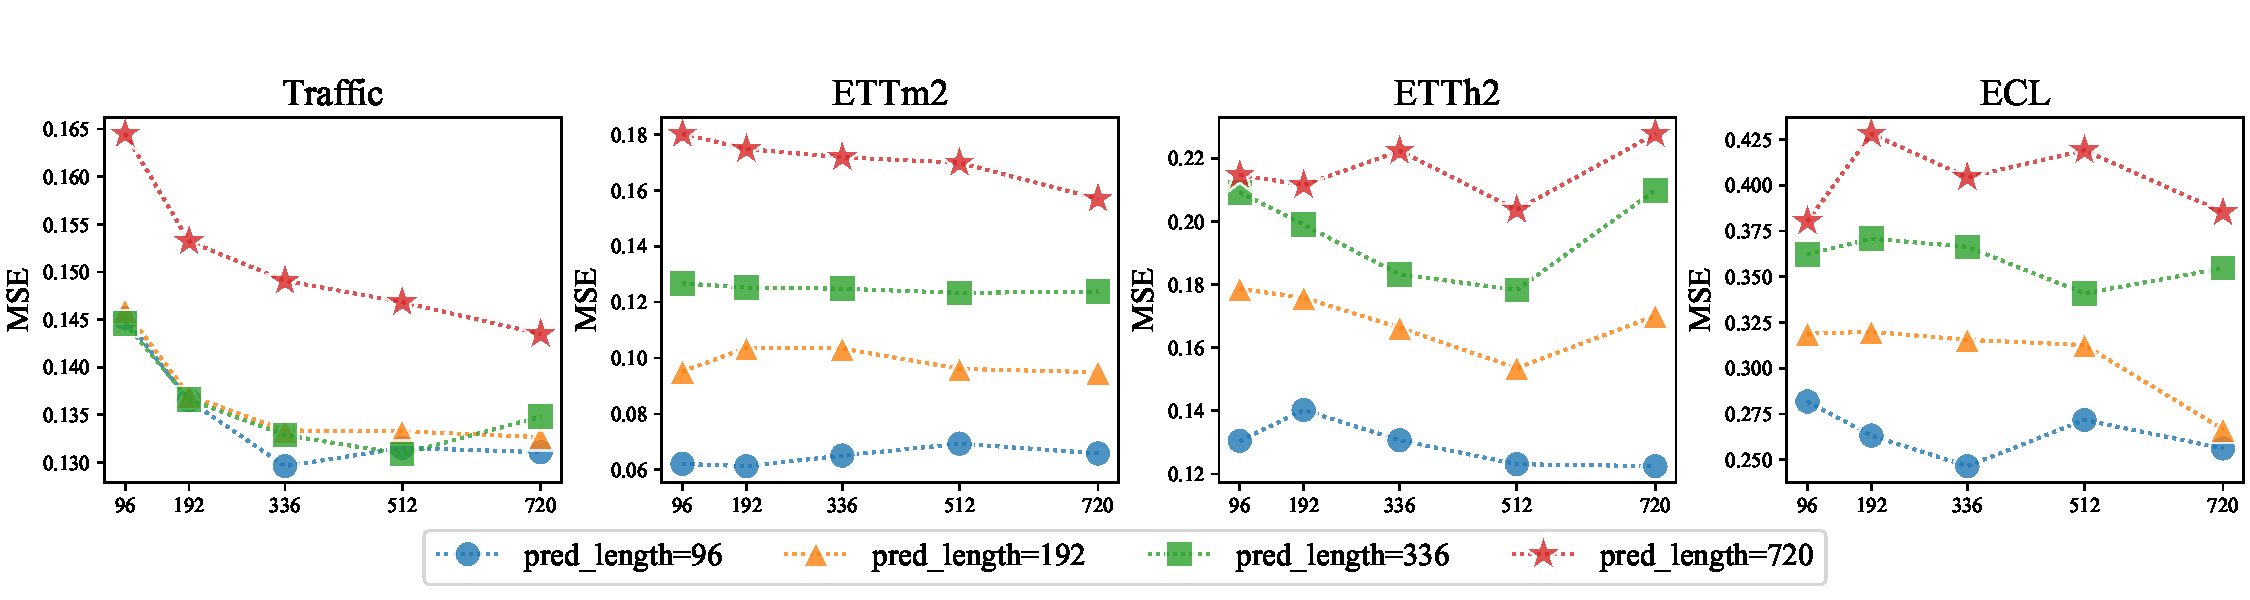
\includegraphics[width=\linewidth]{fig/Increasev2.pdf}
    \vspace{-20pt}
    \caption{Forecasting performance with the look-back length of exogenous variables varying from $\{96, 192, 336, 512, 720\}$ with a fixed look-back length of the endogenous variable to 96. Different styles of lines represent different prediction lengths. In most cases, the forecasting performance benefits from the increase of exogenous look-back length.}
    \vspace{-5pt}
    \label{fig:increase}
\end{figure*}


\paragraph{Representation Analysis} To evaluate the performance of TimeXer from the perspective of representation, we adopt centered kernel alignment (CKA) similarity \cite{kornblith2019similarity} analysis. Previous works \cite{wu2023timesnet, dong2023simmtm} 
reveal that for low-level time series task including forecasting, there is a great similarity among representations from the different layers and a higher similarity corresponds to a better performance. As shown in Figure \ref{fig:cka}, the representations from the first and the last layers of TimeXer enjoy great similarities, verifying that TimeXer can learn the appropriate representations for the prediction. It is notable that iTransformer does not distinguish between endogenous and exogenous variables and the output of the model contains representation of all variables. However, the result of the CKA analysis shows that despite the high similarity of the series representations of all variables, the representation of the endogenous variables was not well learned. This result also suggests that directly applying a multivariate model to perform forecasting with exogenous variables introduces unnecessary noise into the model thus interfering with its forecasting performance.

\begin{figure}[h]
    \vspace{-10pt}
    \centering
    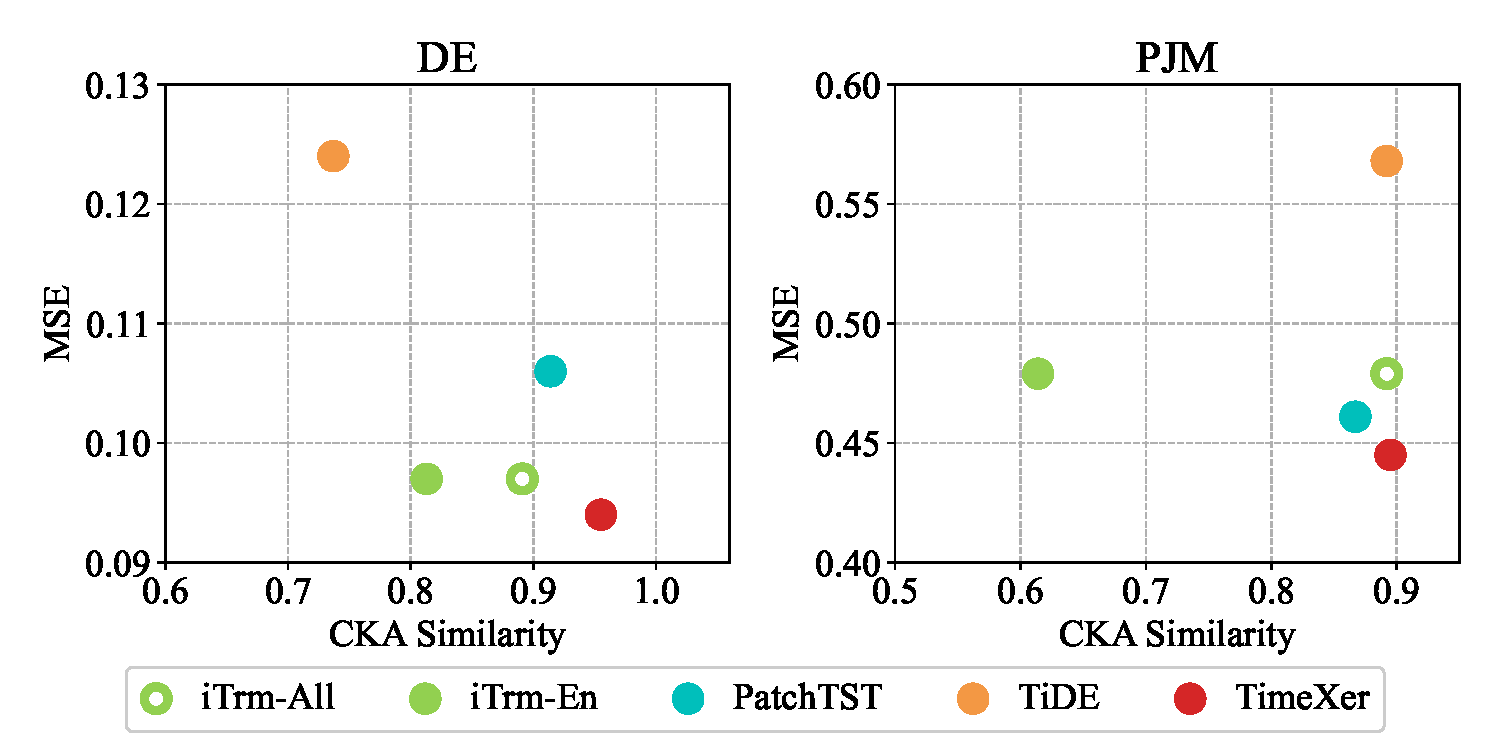
\includegraphics[width=\linewidth]{fig/cka_2.pdf}
    \vspace{-20pt}
    \caption{Comparison of representation CKA similarity between TimeXer and competitive baselines. \emph{iTrm-All} denotes the series representation of all variables learned by iTransformer, \emph{iTrm-En} is the learned series representation of the endogenous variable.}
    \label{fig:cka}
    \vspace{-15pt}
\end{figure}



\paragraph{Increasing Exogenous Look-back Length}
Theoretically, the forecasting performance of the model could potentially benefit from an increased length of the look-back window, as a longer historical context can provide a more comprehensive modeling. However, the attention will be distracted when the window becomes excessively long. In TimeXer, we use the series-level representation of exogenous variables which allows for the misalignment between endogenous and exogenous variables. 
This is particularly valuable in real-world scenarios where the endogenous series may be collected from a newly introduced sensor that has limited historical data. In such cases, using a longer exogenous series can effectively augment the available information for more robust predictions. Based on this motivation, we evaluate the performance of TimeXer in Figure \ref{fig:increase} with increased exogenous look-back length. We fix the length of the endogenous variable to 96 and increase the length of exogenous variables. The results reveal that extending the look-back length of exogenous variables indeed yields improvements in forecasting performance.

\vspace{-10pt}
\paragraph{Extend to Multivariate Forecasting}
The major difference between time series forecasting with exogenous variables and multivariate forecasting lies in the fact that the model does not require predicting the exogenous variables. 
In principle, multivariate forecasting can be viewed as the independent prediction of each variable in multivariate data, and for each variable, the other variables are exogenous to facilitate the prediction.
Motivated by this insight, we endeavored to extend the capabilities of TimeXer to encompass multivariate forecasting scenarios. Technically, we consider the variables in the dataset as mutually independent endogenous variables, with each variable considering all other variables except itself as exogenous variables. 
Leveraging the established long-term multivariate forecasting benchmarks and experimental settings from iTransformer \cite{liu2023itransformer}, we conduct mainstream multivariate forecasting task and evaluate the performance of our proposed TimeXer with state-of-the-art forecasting models. We present the results averaged from all four prediction lengths in Figure \ref{fig:multivariate-result}. It can be observed that TimeXer exhibits competitive performance in multivariate forecasting tasks with baseline models, highlighting its effectiveness and generality.

\begin{figure}[t]
    \vspace{-10pt}
    \centering
    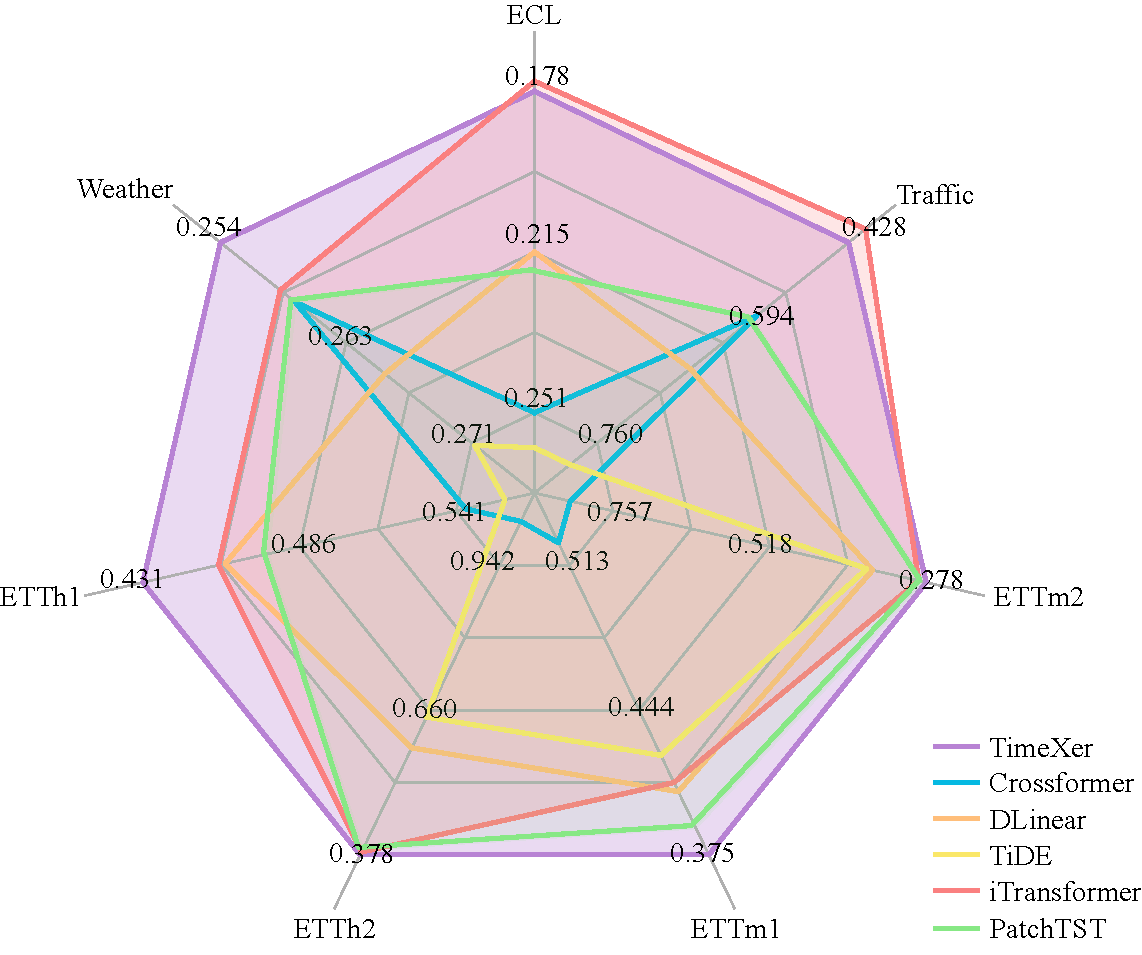
\includegraphics[width=0.7\linewidth]{fig/TimeXer_Radar_MK2.pdf}
    \vspace{-10pt}
    \caption{Performance Comparison between TimeXer with state-of-art models. Full results are listed in Appendix \ref{tab:full-log-multi}.}
    \vspace{-20pt}
    \label{fig:multivariate-result}
\end{figure}
\vspace{-5pt}
\section{Conclusion}
Considering the prevalence of exogenous variables in real-world forecasting scenarios, we empower the canonical Transformer architecture with the ability to reconcile endogenous and exogenous information without architectural modifications. With a deftly designed embedding strategy, our proposed TimeXer is able to capture both endogenous temporal dependencies and multivariate correlations between endogenous and exogenous variables. 
Experimental results demonstrate that our proposed TimeXer achieves state-of-the-art performance in both the short- and long-term forecasting task with exogenous variables.
Going beyond the experimental setting, TimeXer demonstrates its potential in a variety of complex real-world forecasting scenarios containing exogenous variables, including challenges such as low data quality and misalignment between series.


% In the unusual situation where you want a paper to appear in the
% references without citing it in the main text, use \nocite
\nocite{langley00}

\bibliography{ref}
\bibliographystyle{icml2024}


%%%%%%%%%%%%%%%%%%%%%%%%%%%%%%%%%%%%%%%%%%%%%%%%%%%%%%%%%%%%%%%%%%%%%%%%%%%%%%%
%%%%%%%%%%%%%%%%%%%%%%%%%%%%%%%%%%%%%%%%%%%%%%%%%%%%%%%%%%%%%%%%%%%%%%%%%%%%%%%
% APPENDIX
%%%%%%%%%%%%%%%%%%%%%%%%%%%%%%%%%%%%%%%%%%%%%%%%%%%%%%%%%%%%%%%%%%%%%%%%%%%%%%%
%%%%%%%%%%%%%%%%%%%%%%%%%%%%%%%%%%%%%%%%%%%%%%%%%%%%%%%%%%%%%%%%%%%%%%%%%%%%%%%
\newpage
\appendix
\onecolumn
\section{Implementation Details}

\subsection{Dataset Descriptions}
We conduct long-term forecasting experiments on 7 real-world datasets to evaluate the performance of our proposed TimeXer, including: (1) \textbf{ECL} \cite{li2019enhancing} includes hourly electricity consumption data from 321 clients. We take the electricity consumption of the last client as an endogenous variable and other clients as exogenous variables. (2) \textbf{Weather} \cite{zhou2021informer} records 21 meteorological factors collected every 10 minutes from the Weather Station of the Max Planck Biogeochemistry Institute in 2020. In our experiment, we use the Wet Bulb factor as the endogenous variable to be predicted and the other indicators as exogenous variables. (3) \textbf{ETT} \cite{zhou2021informer} contains four subsets where ETTh1 and ETTh2 are hourly recorded, and ETTm1 and ETTm2 are recorded every 15 minutes. The endogenous variable is the oil temperature and the exogenous variables are 6 power load features. (4) \textbf{Traffic} \cite{wu2023timesnet} records hourly road occupancy rates measured by 862 sensors of San Francisco Bay area freeways.  We take the measurement of the last sensor as an endogenous variable and others as exogenous variables.

In addition to the public multivariate time series datasets, we perform short-term forecasting on the Electricity Price Forecasting Datasets \cite{lago2021forecasting}, which contains five datasets representing five different day-ahead electricity markets spanning six years each. Here are the descriptions of the datasets: (1) \textbf{NP} represents The Nord Pool electricity market, recording the hourly electricity price, and corresponding grid load and wind power forecast from 2013-01-01 to 2018-12-24. (2) \textbf{PJM} represents the Pennsylvania-New Jersey-Maryland market, which contains the zonal electricity price in the Commonwealth Edison (COMED), and corresponding System load and COMED load forecast from 2013-01-01 to 2018-12-24. (3) \textbf{BE} represents Belgium's electricity market, recording the hourly electricity price, load forecast in Belgium, and generation forecast in France from 2011-01-09 to 2016-12-31. (4) \textbf{FR} represents the electricity market in France, recording the hourly prices, and corresponding load and generation forecast from 2012-01-09 to 2017-12-31. (5) \textbf{DE} represents the German electricity market, recording the hourly prices, the zonal load forecast in the TSO Amprion zone, and the wind and solar generation forecasts from 2012-01-09 to 2017-12-31.



\begin{table*}[h]
\vspace{-10pt}
\centering
\renewcommand{\arraystretch}{1}
\caption{Dataset descriptions. \emph{Ex.} and \emph{En.} are abbreviations for the Exogenous variable and Endogenous variable, respectively. The dataset size is organized in (Train, Validation, Test)}
\vspace{5pt}
\resizebox{\linewidth}{!}{
\begin{tabular}{cccccc}
\toprule[1.2pt]
Dataset              & \#Num     & Ex. Descriptions                                 & En. Descriptions                 & Sampling Frequency   & Dataset Size   \\ \toprule[1.2pt]
Electricity          & 320                & Electricity Consumption                          & Electricity Consumption          & 1 Hour    &   (18317, 2633, 5261)           \\ \midrule
Weather              & 20                 & Climate Feature                                  & CO2-Concentration                    & 10 Minutes  & (36792, 5271, 10540)           \\ \midrule
ETTh                 & 6                  & Power Load Feature                               & Oil Temperature                  & 1 Hour    & (8545, 2881, 2881)               \\ \midrule
ETTm                 & 6                  & Power Load Feature                               & Oil Temperature                  & 15 Minutes  & (34465, 11521, 11521)            \\ \midrule
Traffic              & 861                & Road Occupancy Rates                             & Road Occupancy Rates             & 1 Hour   & (12185, 1757, 3509)               \\ \midrule
NP                   & 2                  & Grid Load, Wind Power                            & Nord Pool Electricity Price      & 1 Hour    & (36500, 5219, 10460)              \\ \midrule
\multirow{2}{*}{PJM} & \multirow{2}{*}{2} & \multirow{2}{*}{System Load, SyZonal COMED load} & Pennsylvania-New Jersey-Maryland & \multirow{2}{*}{1 Hour} & \multirow{2}{*}{(36500, 5219, 10460)} \\
                     &                    &                                                  & Electricity Price                &         &              \\ \midrule
BE                   & 2                  & Generation, System Load                          & Belgium's Electricity Price      & 1 Hour   & (36500, 5219, 10460)                   \\ \midrule
FR                   & 2                  & Generation, System Load                          & France's Electricity Price       & 1 Hour    & (36500, 5219, 10460)                  \\ \midrule
DE                   & 2                  & Wind power, Ampirion zonal load                  & German's Electricity Price       & 1 Hour    & (36500, 5219, 10460)                  \\ \bottomrule[1.2pt]
\end{tabular}}
\label{tab:full-dataset}
\vspace{-10pt}
\end{table*}
\subsection{Implementation Details}

All the experiments are implemented in PyTorch \cite{paszke2019pytorch} and conducted on a single NVIDIA 4090 24GB GPU. We utilize ADAM \cite{kingma2014adam} with an initial learning rate $10^{-4}$ and L2 loss for the model optimization. The training process is fixed to $10$ epochs with an early stopping. We set the number of TimeXer blocks in our proposed model $L\in\{1, 2, 3\}$. The dimension of series representations $d_{model}$ is searched from $\{128, 256, 512\}$. The patch length is uniformly set to 16 for long-term forecasts and 24 for short-term forecasts. We reproduced the compared baseline models based on the benchmark of TimesNet \cite{wu2023timesnet} Repository.

\section{Model Efficiency}
To evaluate the efficiency of TimeXer, we evaluate the training speed and memory usage of TimeXer with six baseline models with identical hidden dimensions and batch sizes. Specifically, we choose ECL and NP datasets, corresponding to the two representative cases of excessive (320 exogenous variables) and few (2 exogenous variables) variables, respectively. It can be observed that when there are few exogenous variables, our model has no significant advantage in efficiency, but the forecasting performance is optimal. The results indicate that although our model exhibits optimal forecasting performance, there is little efficiency advantage when dealing with a small number of exogenous variables.
It is notable that when faced with numerous variables TimeXer demonstrates its advantage by outperforming iTransformer in terms of memory footprint. This is because, in TimeXer, the Cross-Attention layer learns the dependencies between exogenous and endogenous variables, whereas iTransformer learns the multivariate relationships between all the variables, leading to higher computational complexity.

\begin{figure}[h]
    \centering
    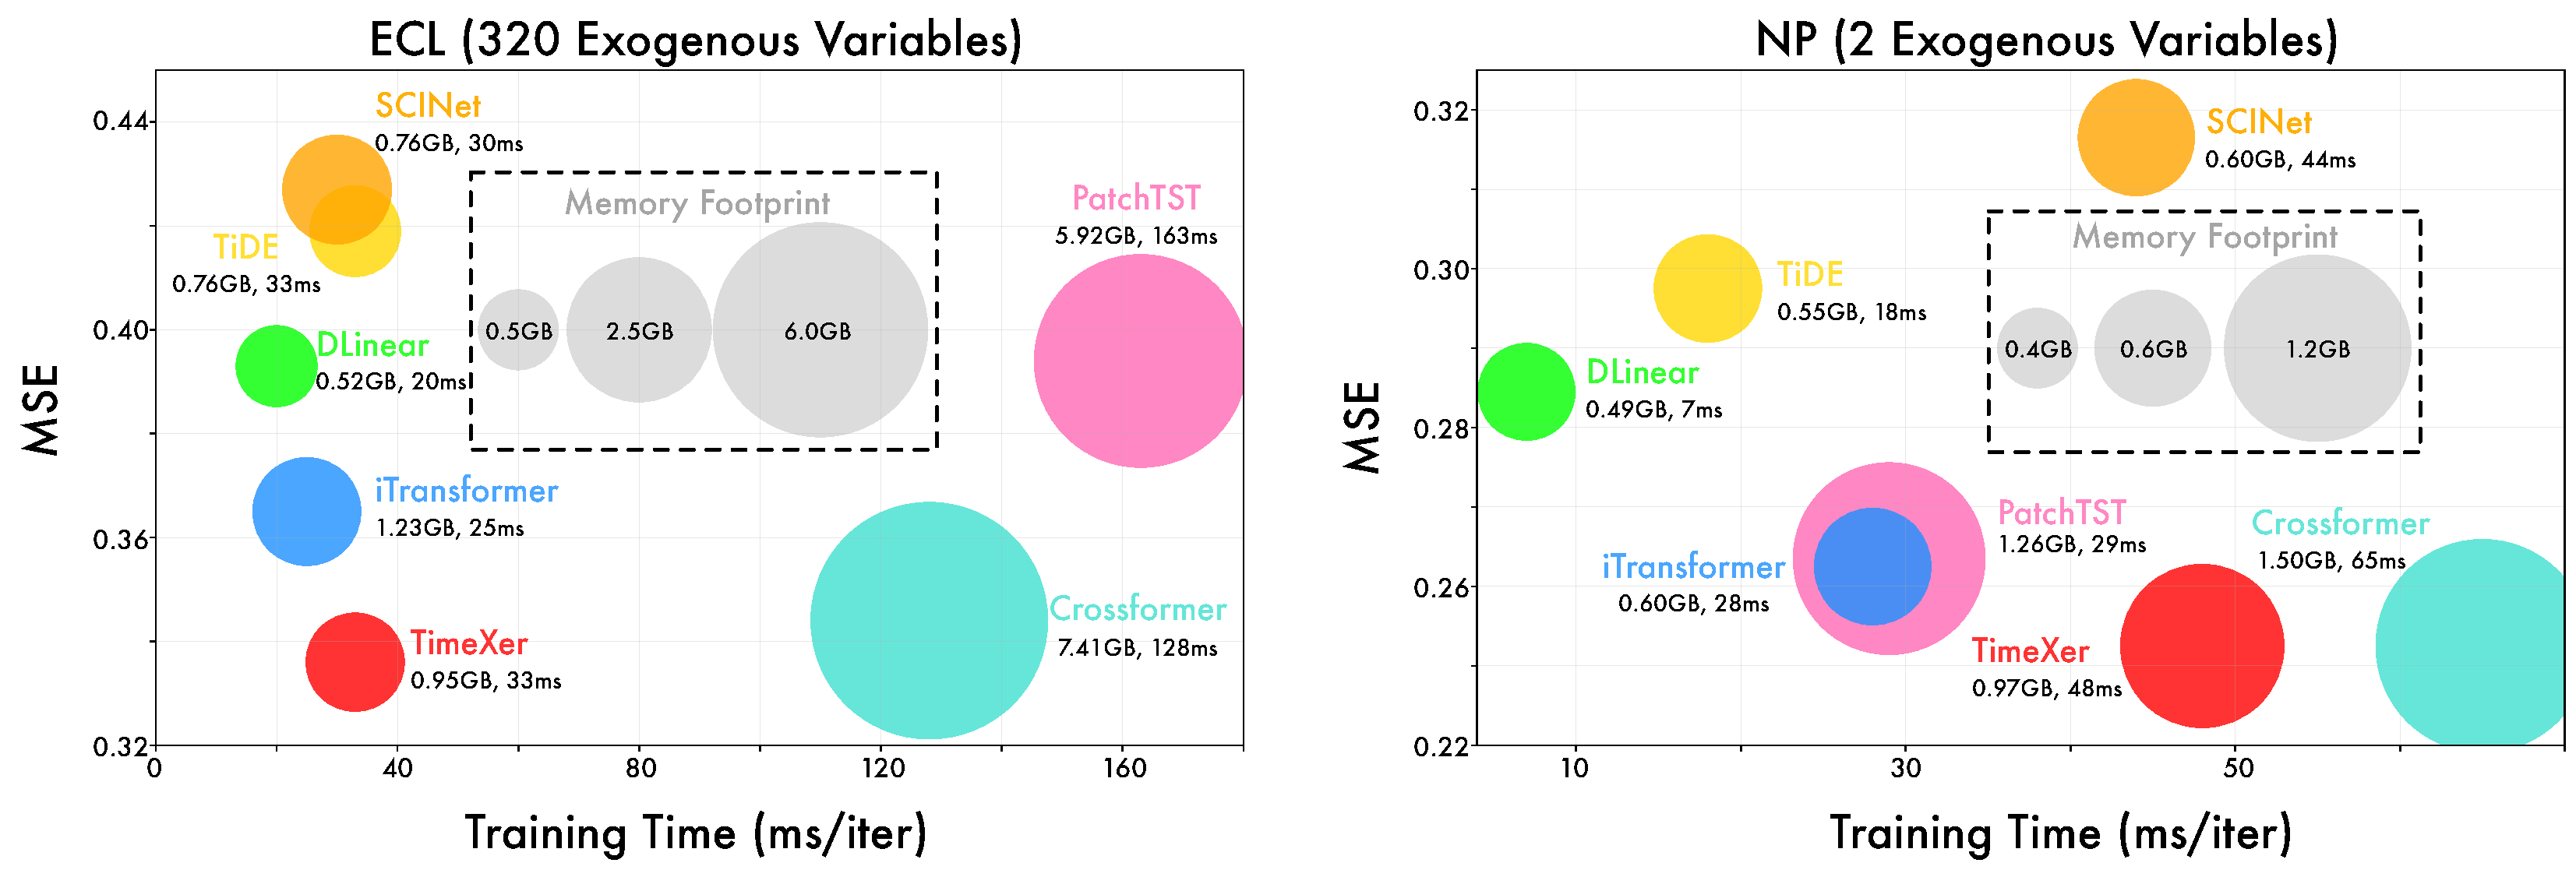
\includegraphics[width=0.8\linewidth]{fig/efficiencyv2.pdf}
    \caption{Model efficiency comparison on ECL and NP datasets.}
    \vspace{-20pt}
    \label{fig:enter-label}
\end{figure}



\section{Ablation Study}
\subsection{Varying Patch Length}
In this section, we experiment with the effect of patch lengths on the forecasting performance. We fix the look-back window to 96 and vary the patch lengths $P \in \{4, 6, 8, 12, 16, 24\}$. We conduct experiments on all datasets with consistent parameters except patch-length, and the results are shown in Figure \ref{fig:patch-len}. The results are the averaged MSE under four different prediction length $S \in \{96, 192, 336, 720\}$. It can be seen that the average prediction performance does not vary dramatically with different patch lengths, which indicates that our model is robust to the patch length hyperparameter. Notably, the model generally performs lower when the patch length is small, which is probably because small patches are not enough to represent the semantic information in time series data.


\begin{figure}[h]
    \centering
    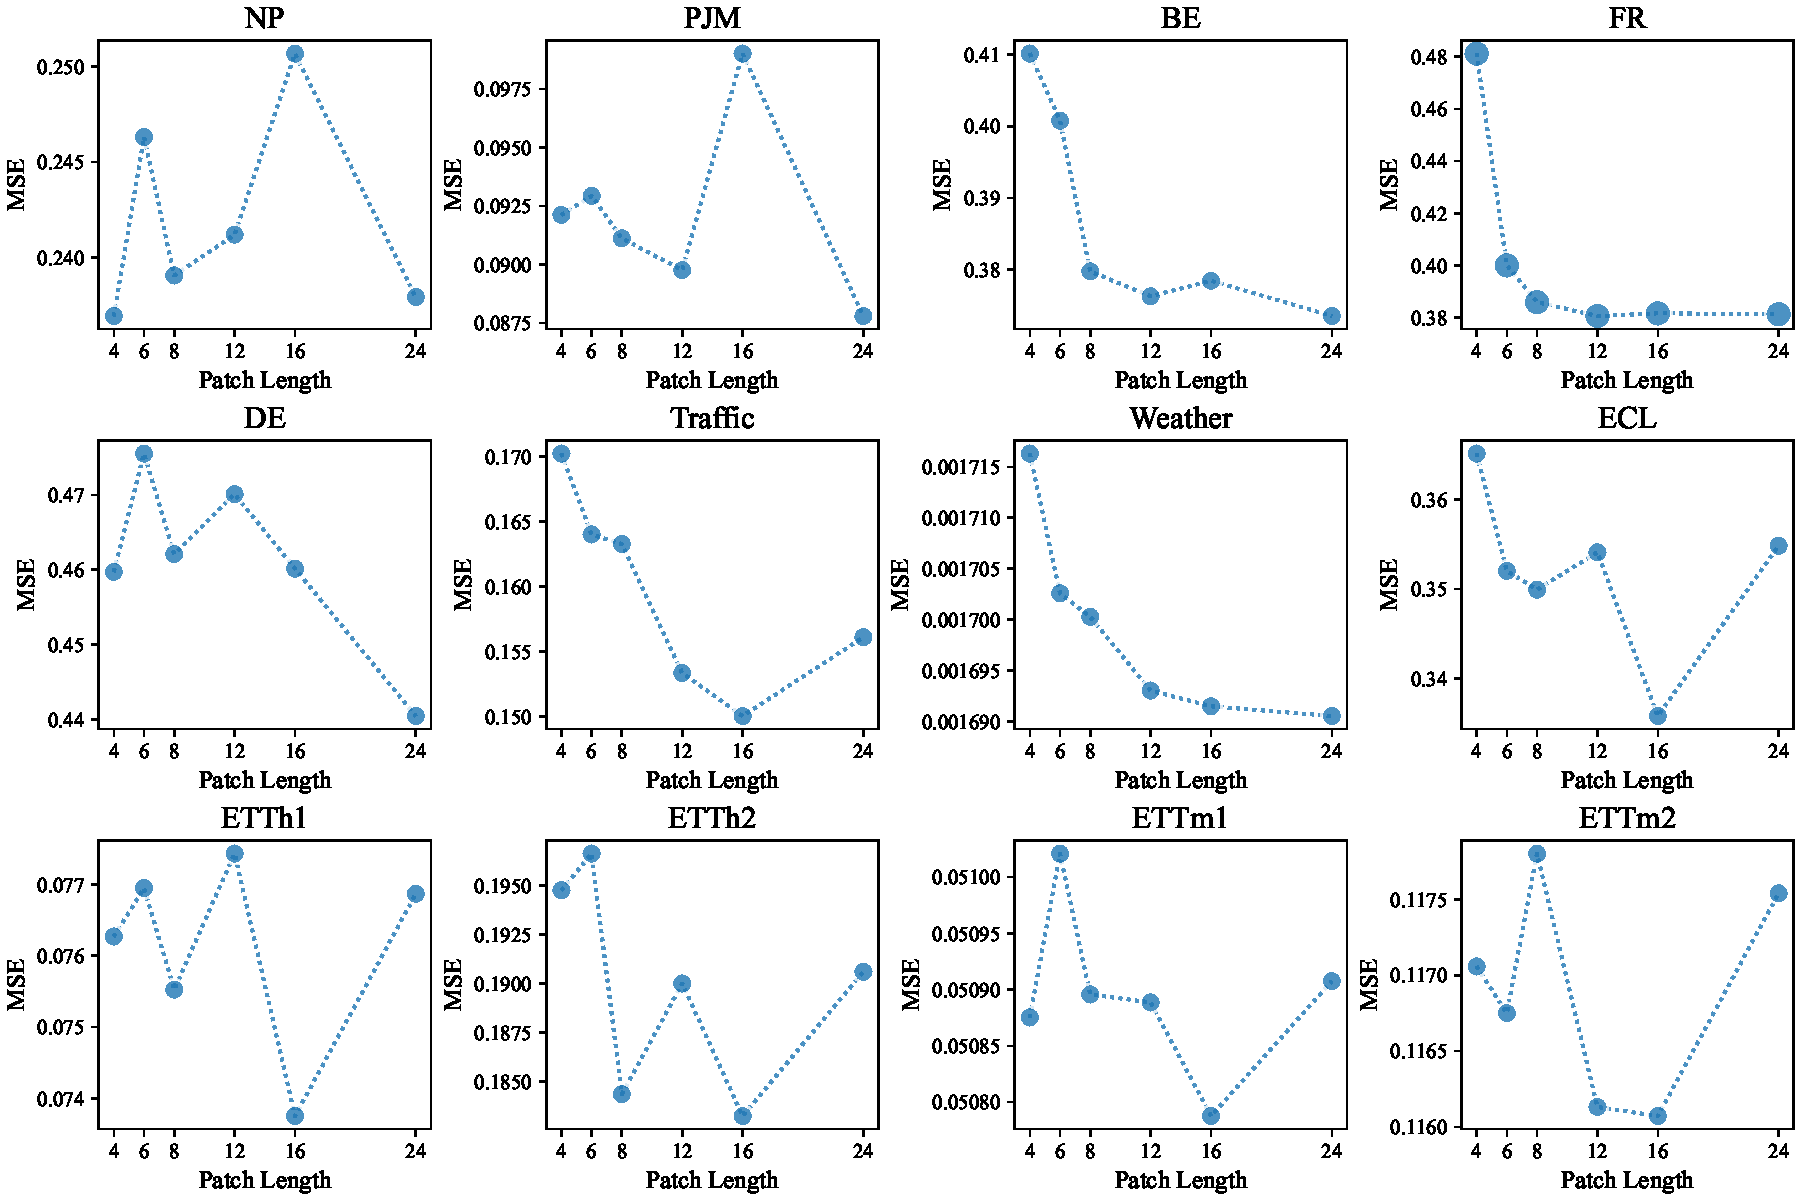
\includegraphics[width=\linewidth]{fig/patch-len.pdf}
    \vspace{-5px}
    \caption{Hyper-parameter sensitivity analysis of TimeXer on twelve real-world forecasting benchmarks.}
    \label{fig:patch-len}
\end{figure}



\subsection{Varying Different Embedding}

In our above-mentioned analysis, we apply different embedding strategies to the endogenous and exogenous variables. For the endogenous variable, we apply patch embedding and variate embedding to capture both temporal dependencies and cross-attention between different variables. To verify the rationality of this setting, we select two additional settings. First, we replace variate embedding with patch embedding on exogenous variables, while keeping the embedding strategy on the endogenous variable fixed. Second, we modify the embedding design on the endogenous variable by removing either temporal embedding or patch embedding. We calculate the average MSE loss on four different prediction lengths to fully evaluate the performance of each setting.

\textbf{Temporal dependencies and cross-attention are both important in the endogenous variable embedding.} Our numerical experiments in Table \ref{tab:abalation} verify that taking down either kind of embedding from the endogenous variable weakens the averaged performance. Precisely, the two different embedding choices can be seen as two independent threads of the forecasting process. First, we believe that the evolving trend of a time-series variable in the future shall follow the trend that it has been following in the past. The patch embedding gains the temporal dependencies of how the endogenous variable itself has been evolving, which is important evidence of the future evolution of this endogenous variable. Second, we also believe that the evolving trend of a time-series variable shall be strongly related to its covariant. In Transformer-based deep learning models, researchers found cross-attention a powerful tool to estimate variable relations. The variate embedding gains the cross-attention between the endogenous variable and all exogenous variables, which is important evidence of how exogenous variables are influencing the endogenous variable during evolution. By combining these two kinds of information, we achieve better average performance than using only one kind on most datasets.

\textbf{Cross-attention information of exogenous variables leads to better performance generally.} When replacing patch embedding with temporal embedding, the average MSE loss slightly rises compared to our original design. This indicates that extracting cross-attention information from all exogenous variables better is more beneficial than perceiving temporal dependencies for most time-series learning tasks. Intuitively, exogenous variables serve as background information for forecasting the endogenous variables. Thus, the model should learn the relationship between exogenous variables and the specific endogenous variable to achieve better performance. In this case, we use cross-attention to represent the correlation between different exogenous variables, which we believe has enabled better construction of this endogenous-exogenous variable relation during the machine learning process. Temporal embedding, however, is not able to learn the correlation between different variables, which leads to this performance decline in Table \ref{tab:abalation}.

\begin{table}[h]
\centering
\renewcommand{\arraystretch}{0.85}
\caption{Full results of the ablation study.}
\vspace{2pt}
\setlength{\tabcolsep}{4pt}
\begin{sc}
\resizebox{0.9\linewidth}{!}{
\begin{tabular}{c|c|c|c|cc|cc|cc}
\toprule[1.2pt]
\multirow{2}{*}{Design} & \multirow{2}{*}{Endogenous} & \multirow{2}{*}{Exogenous} & \multirow{2}{*}{Horizon} & \multicolumn{2}{c}{ETTh2} & \multicolumn{2}{c}{ETTm2} & \multicolumn{2}{c}{Traffic} \\
\cmidrule(lr){5-6}\cmidrule(lr){7-8}\cmidrule(lr){9-10}
 &  &  &  & MSE & MAE & MSE & MAE & MSE & MAE \\ \toprule[1.2pt]
\multirow{5}{*}{Ours} & \multirow{5}{*}{Temporal+Variate} & \multirow{5}{*}{Variate} & 96 & 0.130 & 0.278 & 0.062 & 0.180 & 0.145 & 0.219 \\
 &  &  & 192 & 0.179 & 0.330 & 0.095 & 0.229 & 0.146 & 0.220 \\
 &  &  & 336 & 0.209 & 0.366 & 0.127 & 0.270 & 0.145 & 0.224 \\
 &  &  & 720 & 0.215 & 0.372 & 0.180 & 0.330 & 0.165 & 0.246 \\
 &  &  & Avg & \textbf{0.183} & \textbf{0.337} & \textbf{0.116} & \textbf{0.252} & \textbf{0.150} & \textbf{0.227} \\ \midrule
\multirow{5}{*}{Replace} & \multirow{5}{*}{Temporal+Variate} & \multirow{5}{*}{Temporal} & 96 & 0.131 & 0.279 & 0.067 & 0.186 & 0.155 & 0.234 \\
 &  &  & 192 & 0.180 & 0.332 & 0.100 & 0.235 & 0.152 & 0.231 \\
 &  &  & 336 & 0.222 & 0.375 & 0.135 & 0.280 & 0.151 & 0.233 \\
 &  &  & 720 & 0.234 & 0.387 & 0.185 & 0.335 & 0.174 & 0.258 \\
 &  &  & Avg & 0.192 & 0.343 & 0.122 & 0.259 & 0.158 & 0.239 \\ \midrule
\multirow{10}{*}{w/o} & \multirow{5}{*}{w/o Variate} & \multirow{5}{*}{Variate} & 96 & 0.132 & 0.279 & 0.064 & 0.183 & 0.153 & 0.230 \\
 &  &  & 192 & 0.183 & 0.335 & 0.099 & 0.236 & 0.152 & 0.230 \\
 &  &  & 336 & 0.221 & 0.375 & 0.127 & 0.270 & 0.151 & 0.234 \\
 &  &  & 720 & 0.249 & 0.398 & 0.179 & 0.329 & 0.175 & 0.260 \\
 &  &  & Avg & 0.197 & 0.347 & 0.117 & 0.255 & 0.158 & 0.239 \\
 \cmidrule(lr){2-10}
 & \multirow{5}{*}{w/o Temporal} & \multirow{5}{*}{Variate} & 96 & 0.133 & 0.282 & 0.063 & 0.183 & 0.149 & 0.226 \\ 
 &  &  & 192 & 0.176 & 0.329 & 0.097 & 0.234 & 0.147 & 0.224 \\
 &  &  & 336 & 0.211 & 0.367 & 0.129 & 0.275 & 0.145 & 0.230 \\
 &  &  & 720 & 0.234 & 0.387 & 0.181 & 0.332 & 0.166 & 0.251 \\
 &  &  & Avg & 0.188 & 0.341 & 0.118 & 0.256 & 0.152 & 0.233 
 \\ \bottomrule[1.2pt]
\end{tabular}}
\end{sc}
\end{table}

Our original design of embedding strategy is motivated by our innovative cognitive pattern of beneficial influential factors in forecasting tasks. By using this form of embedding setting, we attempt to make Transformer models learn temporal dependencies of the foretasted endogenous variable on one hand while learning the cross-attention relations between endogenous and exogenous variables on the other hand. We also make the model possess the cross-attention correlation between different exogenous variables at the same time to help the model better understand the relations between endogenous and exogenous variables. The results of this ablation study provide a solid factual basis for our viewpoint. 




\section{Showcase}
To have an intuitive concept of the forecasting process, we visually present endogenous and exogenous variables from selected datasets \textbf{BE}, \textbf{DE}, and \textbf{PJM} in Figure \ref{fig:showBE}, Figure \ref{fig:showDE}, and Figure \ref{fig:showPJM}. In each example, we take down the ground truth values of endogenous and exogenous variables in datasets, as well as the forecasting results of the endogenous variable. Our examples cover six different models: TimeXer, Crossformer, iTransformer, PatchTST, TiDE, and DLinear. All models take in a sequence of data with a length of 168 and perform forecasting tasks on a prediction length of 24. Points of inflection on curves are used to evaluate the forecasting quality. If the predicted value remains within a range of 0.05 compared to the ground truth, we take this prediction as a successful forecast and put a green circle of 0.05 radius around it. Otherwise, we take this prediction as an out-of-range forecast and put a red circle of 0.05 radius to mark its failure.

\begin{figure}[h]
    \centering
    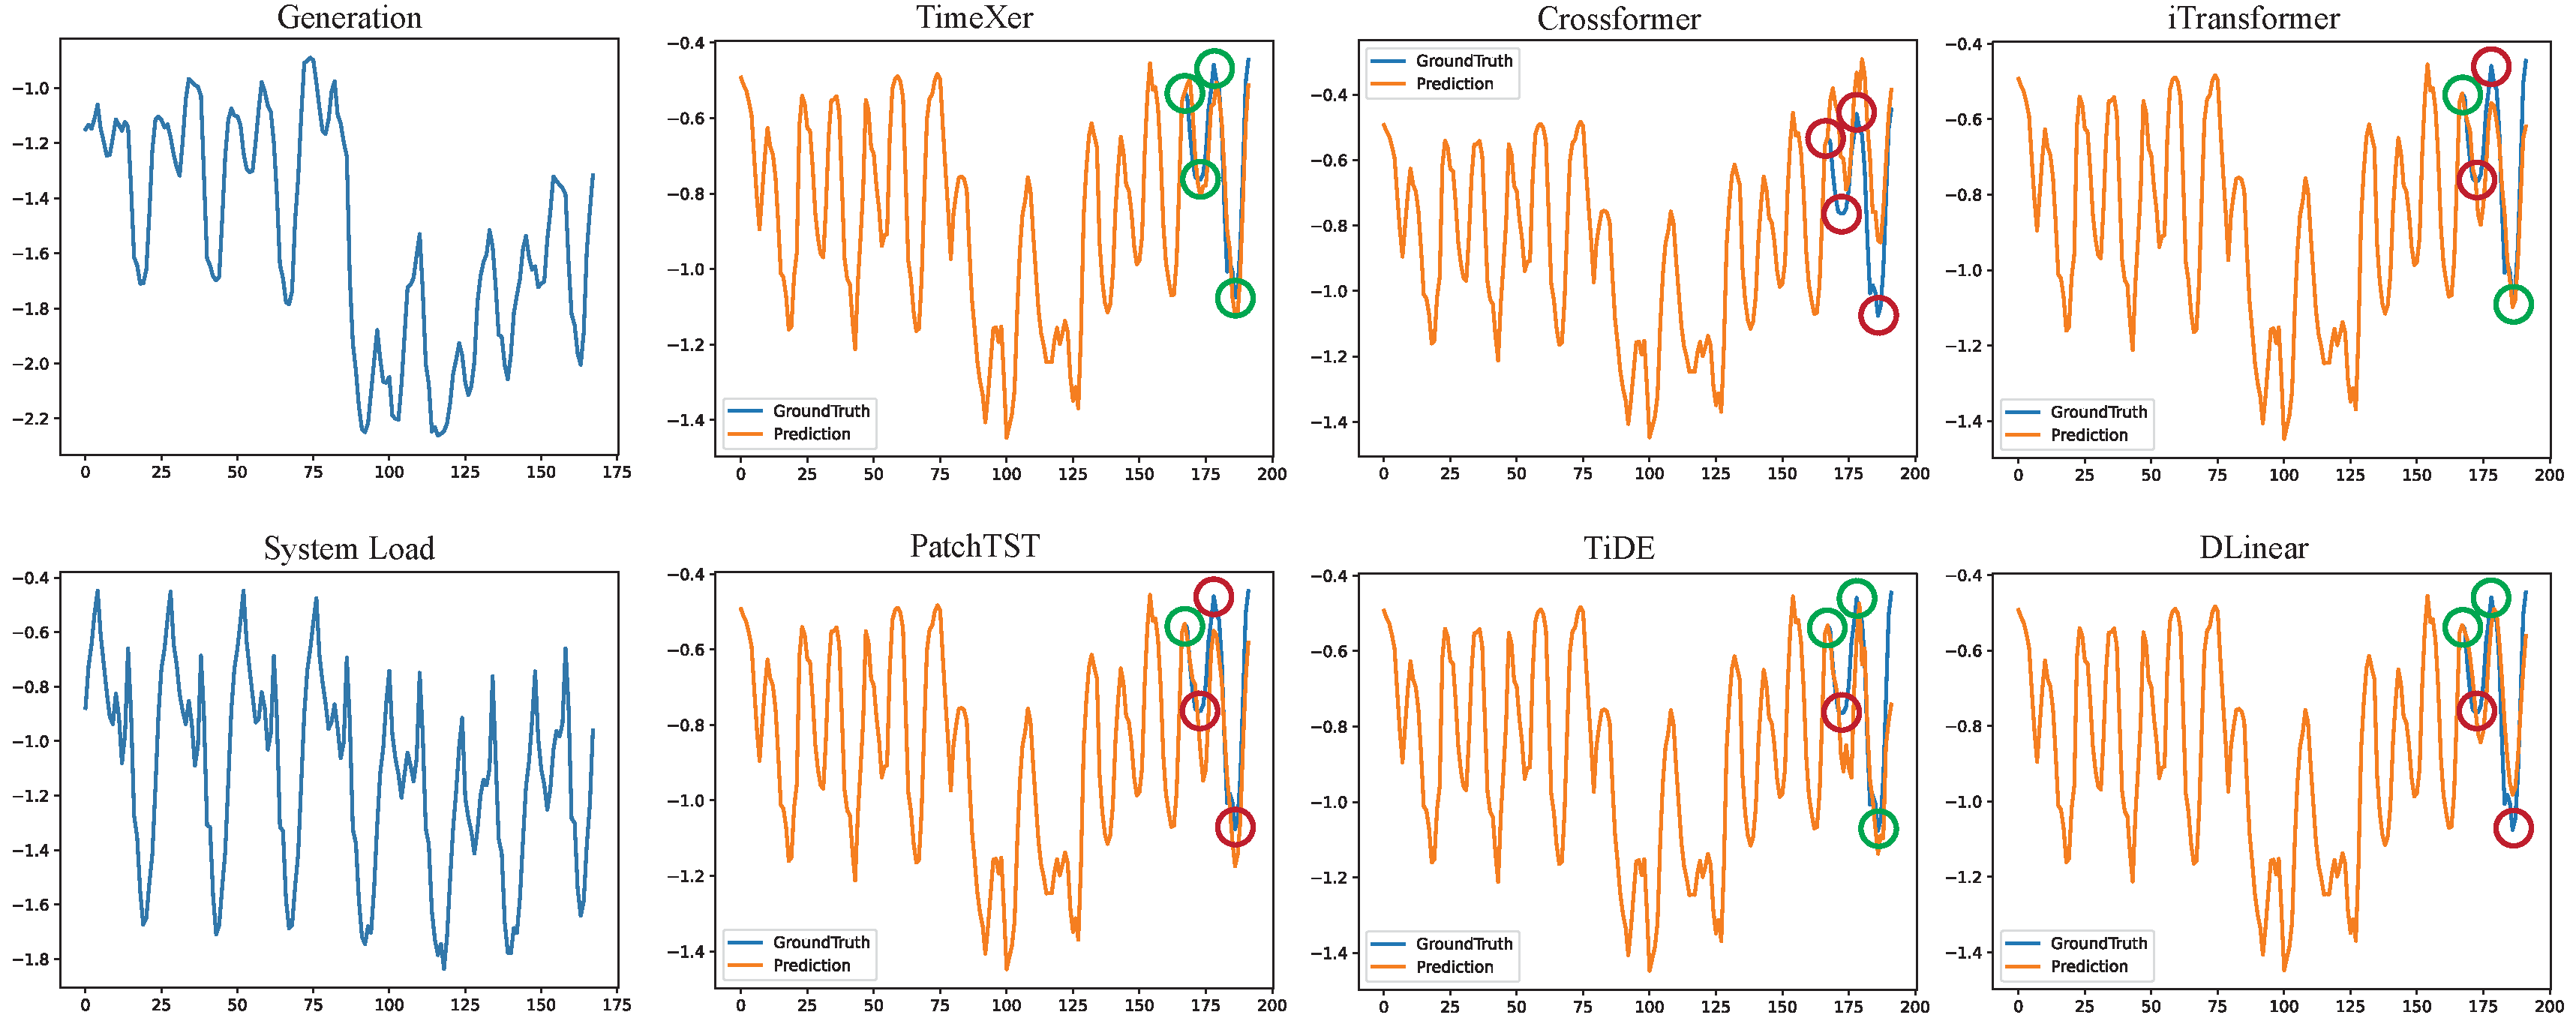
\includegraphics[width=\linewidth]{fig/TimeXer_Showcase_BE_7180.pdf}
    \vspace{-20pt}
    \caption{Showcases of TimeXer in forecasting with exogenous variables from \textbf{BE} datasets. The two leftmost plots of the title "Generation" and "System Load" are the exogenous variables in the \textbf{BE} dataset. TimeXer outperforms all of its challengers by predicting all 4 injections in 24 prediction time points.}
    \label{fig:showBE}
\end{figure}

\begin{figure}[!htbp]
    \centering
    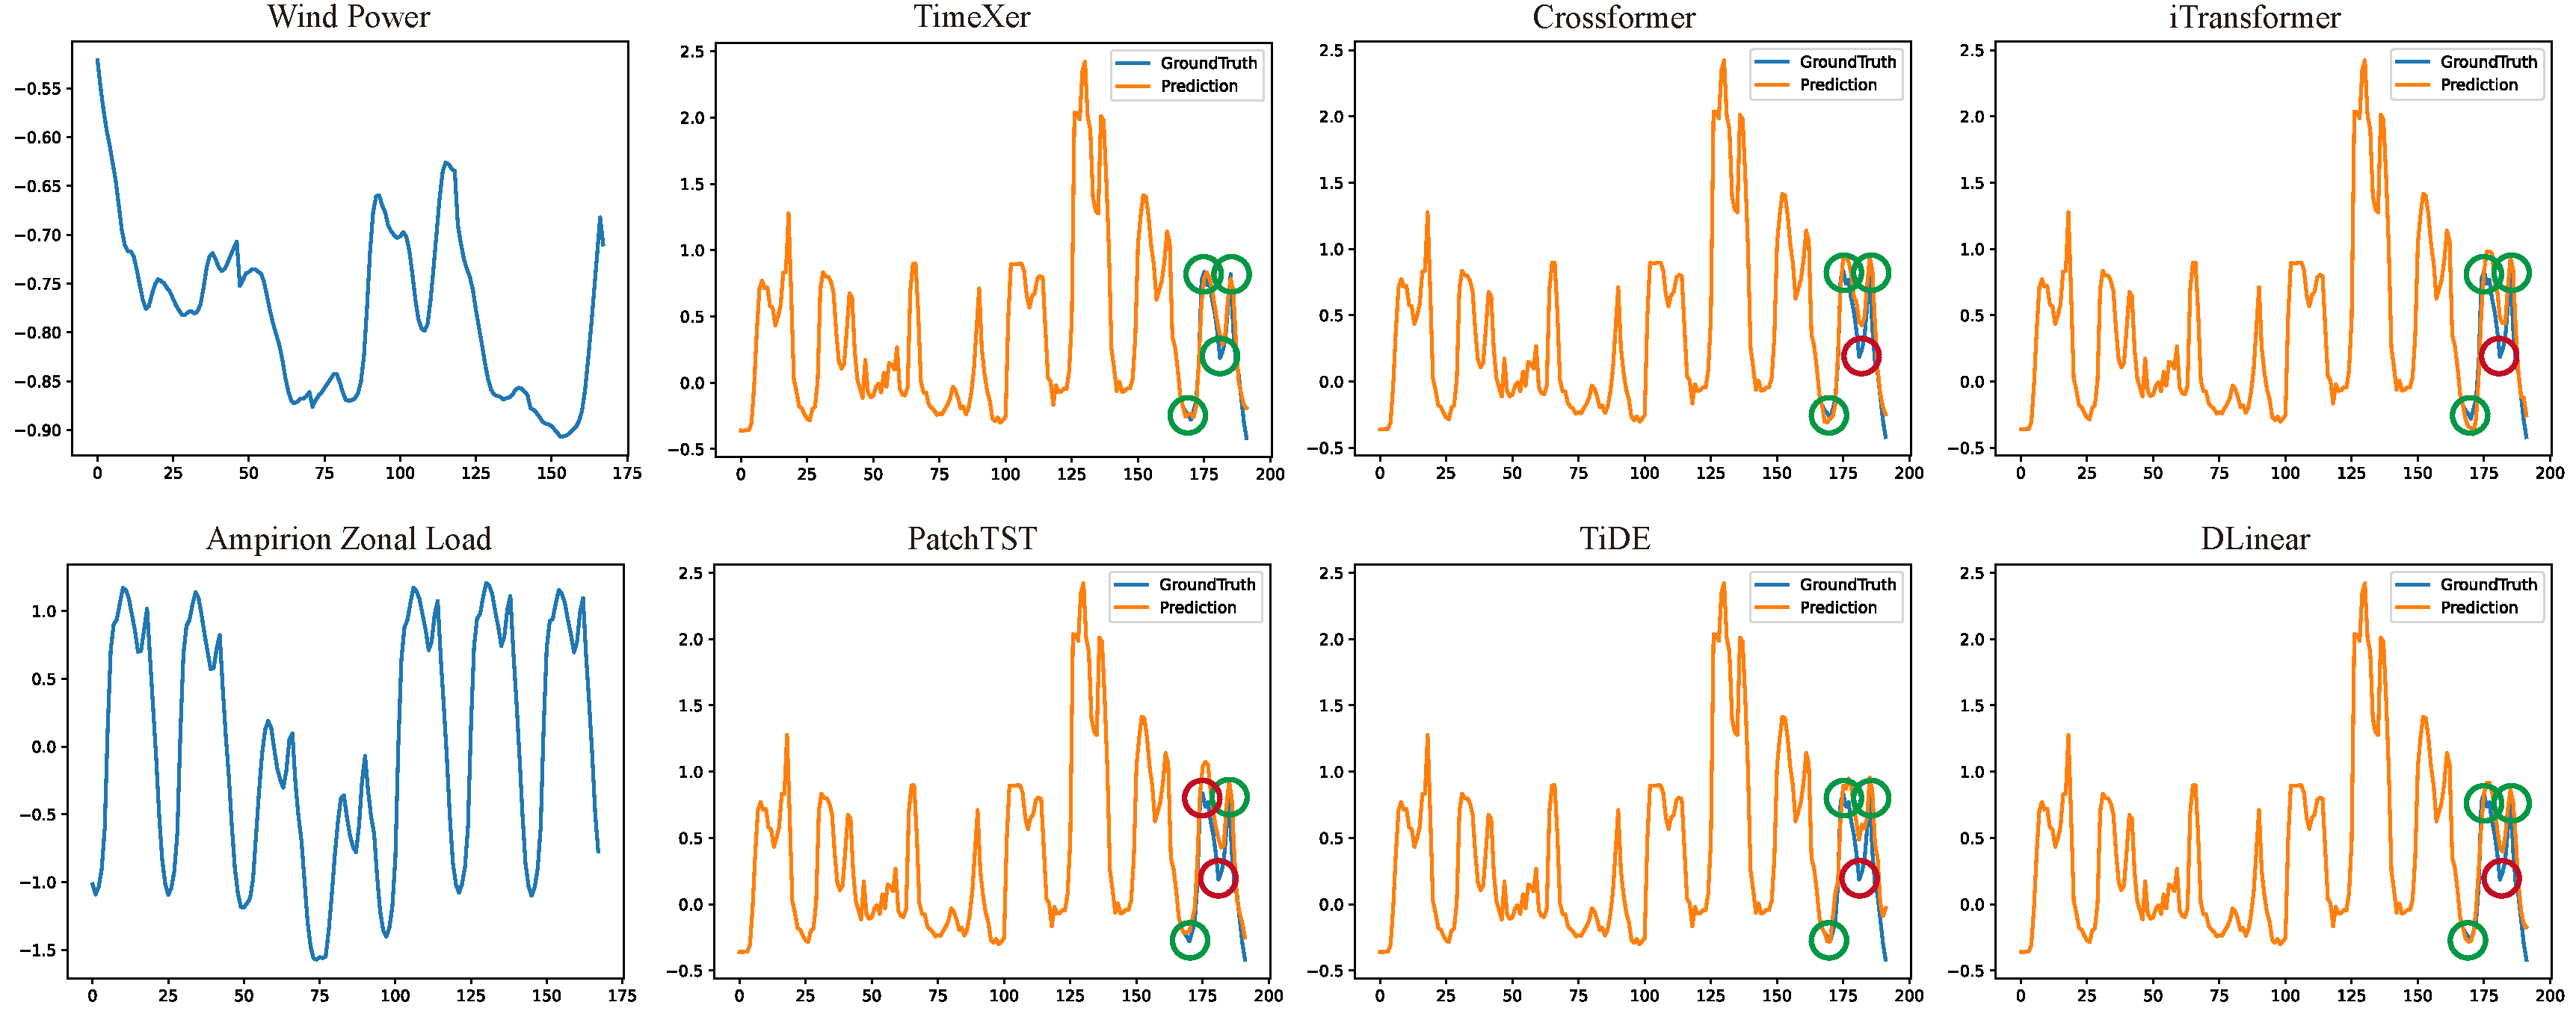
\includegraphics[width=\linewidth]{fig/TimeXer_Showcase_DE_140.pdf}
    \vspace{-20pt}
    \caption{Showcases of TimeXer in forecasting with exogenous variables from \textbf{DE} datasets. The two leftmost plots of the title "System Load" and "Zonal COMED Load" are the exogenous variables in the \textbf{DE} dataset. TimeXer outperforms all of its challengers by predicting all 4 injections in 24 prediction time points.}
    \label{fig:showDE}
\end{figure}

\begin{figure}[!htbp]
    \centering
    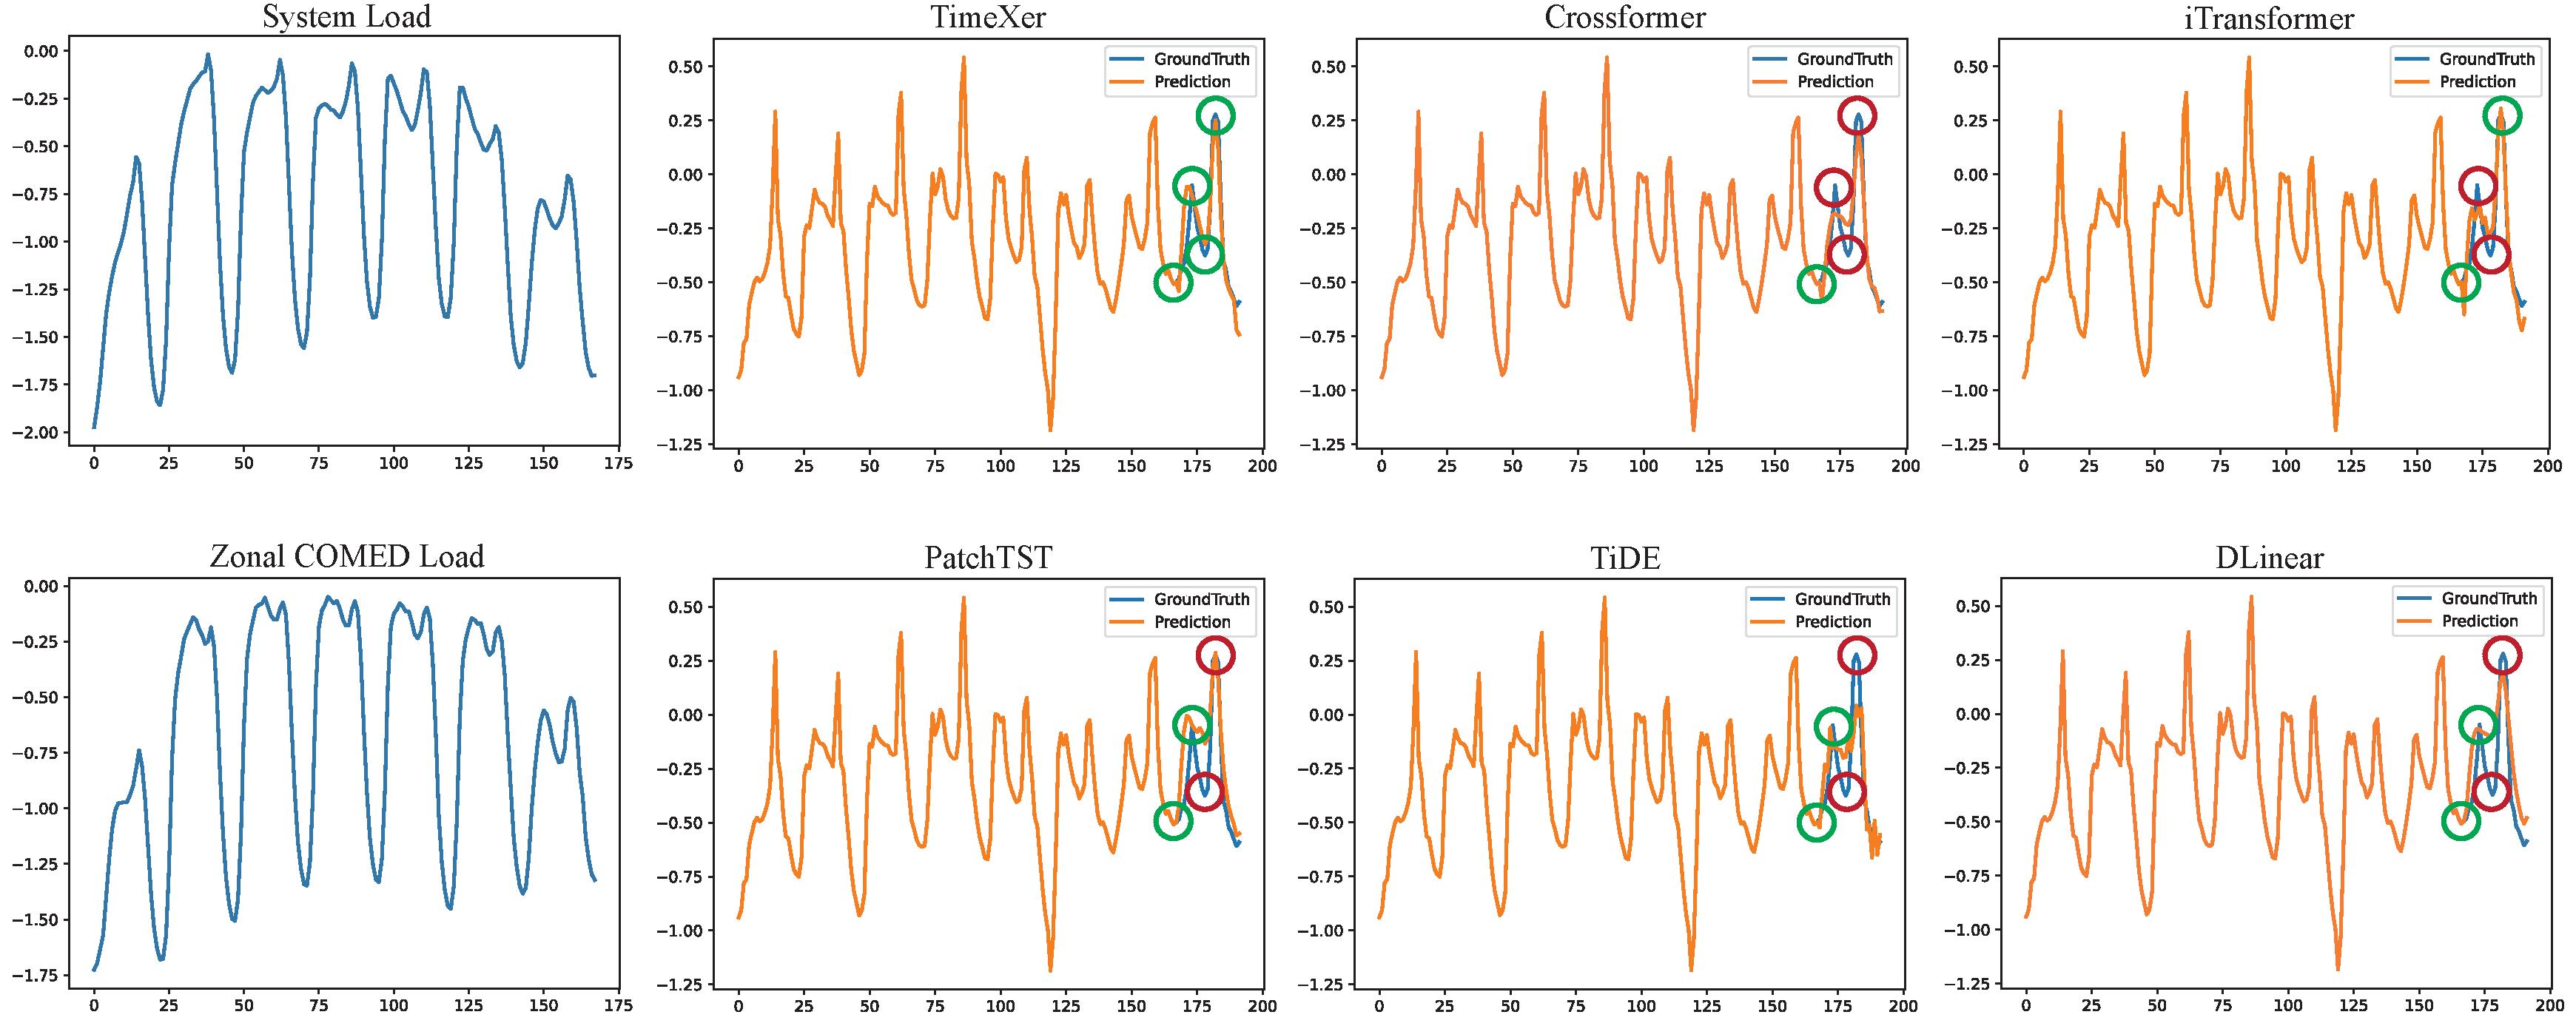
\includegraphics[width=\linewidth]{fig/TimeXer_Showcase_PJM_360.pdf}
    \vspace{-20pt}
    \caption{Showcases of TimeXer in forecasting with exogenous variables from \textbf{PJM} datasets. The two leftmost plots of the title "System Load" and "Zonal COMED Load" are the exogenous variables in the \textbf{PJM} dataset. TimeXer outperforms all of its challengers by predicting all 4 injections in 24 prediction time points.}
    \label{fig:showPJM}
\end{figure}


By counting the green and red circles on all injection points in Figure \ref{fig:showBE}, Figure \ref{fig:showDE}, and Figure \ref{fig:showPJM}, it is clear that the TimeXer can forecast target endogenous more precisely, especially at inflection points where we marked with green circles. Other models tend to vibrate nearby or go beyond the ground truth, indicating that TimeXer is more robust than existing models. By learning from the endogenous variable's temporal dependencies and relations between endogenous and exogenous variables, TimeXer not only acquires abundant contextual information about its own history but also obtains nutritive relation information about correlated variables. Such structure makes TimeXer more aware of the potential pattern of the target dataset, leading to enhanced forecasting performance compared to known Transformer-based models.





\section{Full Results}

Due to the limited space of the main text, all the experiment results are summarized into CKA analysis, long-term forecasting results, and long-term multivariate forecasting results. The CKA analysis is neatly presented in Figure \ref{fig:enter-label}. The two forecasting results are categorized and indexed in Table \ref{tab:full-log} and Table \ref{tab:full-log-multi}.

\subsection{Full Results of CKA Analysis}
o evaluate the performance of TimeXer from the perspective of representation, we adopt centered kernel alignment (CKA) similarity \cite{kornblith2019similarity} analysis. Due to the paper limit,  we provide results from three EPF datasets here.
As shown in Fig. (ref{fig:cka}), the representations of the first and last layers of TimeXer have a great similarity, reaching more than 80\% on all datasets, which verifies that TimeXer is able to learn appropriate representations for prediction.

\begin{figure}[h]
    \centering
    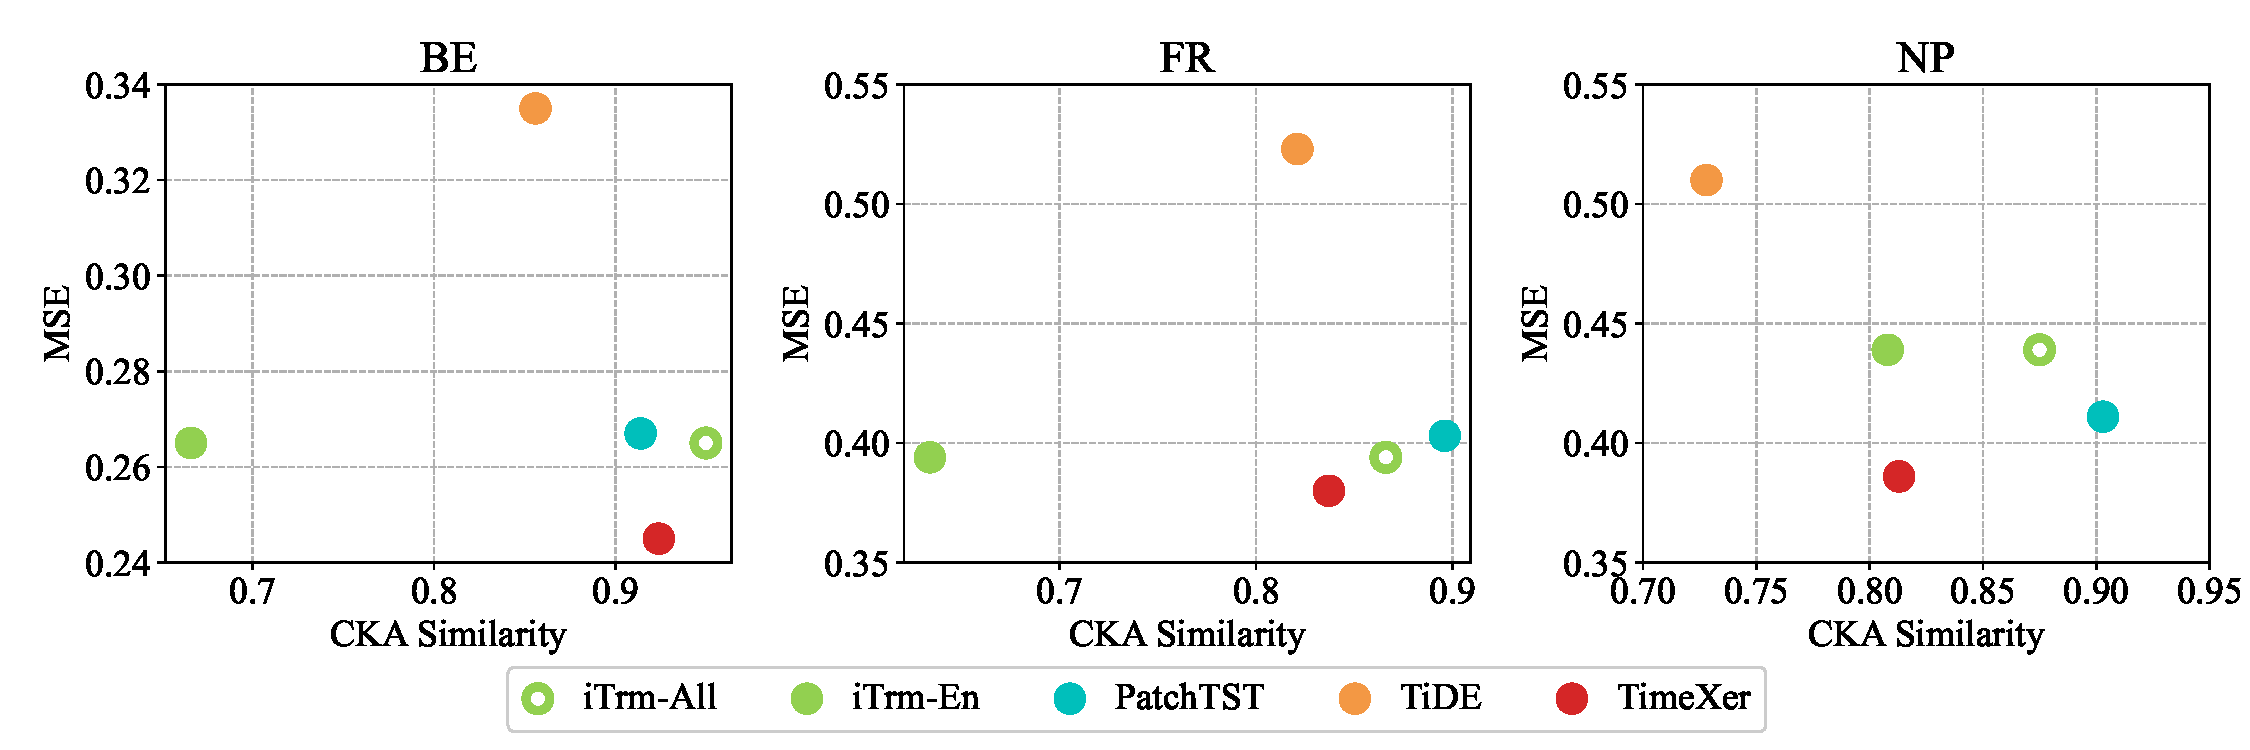
\includegraphics[width=\linewidth]{fig/cka_3.pdf}
    \caption{Series Representation Analysis on three EPF datasets. \emph{iTrm-All} denotes the series representation of all variables learned by iTransformer, \emph{iTrm-En} is the learned series representation of the endogenous variable.}
    \label{fig:full-cka}
\end{figure}


\subsection{Full Results of Long-term Forecasting}
To evaluate the performance of our proposed TimeXer, we conduct long-term forecasting with exogenous variables on acknowledged real-world multivariate datasets. The look-back length is set to 96, and the prediction length varies from $\{96, 192, 336, 720\}$. The results are listed in Table \ref{tab:full-log}.

\begin{table}[h]
\caption{Full results of the long-term forecasting with exogenous variables task.}
\vspace{2pt}
\setlength{\tabcolsep}{2.5pt}
\renewcommand{\arraystretch}{1.5}
\begin{sc}
\resizebox{\linewidth}{!}{
\begin{tabular}{c|c|cc|cc|cc|cc|cc|cc|cc|cc|cc|cc|cc}
\toprule[1.2pt]  
\multicolumn{2}{c}{\multirow{2}{*}{\scalebox{1.35}{Models}}}   & \multicolumn{2}{c}{\scalebox{1.35}{TimeXer}} & \multicolumn{2}{c}{\scalebox{1.35}{iTrans.}} & \multicolumn{2}{c}{\scalebox{1.35}{RLinear}} & \multicolumn{2}{c}{\scalebox{1.35}{PatchTST}} & \multicolumn{2}{c}{\scalebox{1.35}{Cross.}} & \multicolumn{2}{c}{\scalebox{1.35}{TiDE}} & \multicolumn{2}{c}{\scalebox{1.35}{TimesNet}} & \multicolumn{2}{c}{\scalebox{1.35}{DLinear}} & \multicolumn{2}{c}{\scalebox{1.35}{SCINet}} & \multicolumn{2}{c}{\scalebox{1.35}{Stationary}} & \multicolumn{2}{c}{\scalebox{1.35}{Auto.}}  \\ 
\multicolumn{2}{c}{} & \multicolumn{2}{c}{\scalebox{1.35}{(Ours)}} & \multicolumn{2}{c}{\scalebox{1.35}{\citeyearpar{liu2023itransformer}}} & \multicolumn{2}{c}{\scalebox{1.35}{\citeyearpar{li2023revisiting}}} & \multicolumn{2}{c}{\scalebox{1.35}{\citeyearpar{nie2022time}}} & \multicolumn{2}{c}{\scalebox{1.35}{\citeyearpar{zhang2022crossformer}}} & \multicolumn{2}{c}{\scalebox{1.35}{\citeyearpar{das2023long}}} & \multicolumn{2}{c}{\scalebox{1.35}{\citeyearpar{wu2023timesnet}}} & \multicolumn{2}{c}{\scalebox{1.35}{\citeyearpar{zeng2023transformers}}} & \multicolumn{2}{c}{\scalebox{1.35}{\citeyearpar{liu2022scinet}}} & \multicolumn{2}{c}{\scalebox{1.35}{\citeyearpar{liu2022non}}} & \multicolumn{2}{c}{\scalebox{1.35}{\citeyearpar{wu2021autoformer}}} \\ 
\cmidrule(lr){3-4}\cmidrule(lr){5-6}\cmidrule(lr){7-8}\cmidrule(lr){9-10}\cmidrule(lr){11-12}\cmidrule(lr){13-14}\cmidrule(lr){15-16}\cmidrule(lr){17-18}\cmidrule(lr){19-20}\cmidrule(lr){21-22}\cmidrule(lr){23-24}
\multicolumn{2}{c}{\scalebox{1.35}{Metric}}   & \scalebox{1.35}{MSE} & \scalebox{1.35}{MAE} & \scalebox{1.35}{MSE}    & \scalebox{1.35}{MAE}   & \scalebox{1.35}{MSE}    & \scalebox{1.35}{MAE}    & \scalebox{1.35}{MSE}    & \scalebox{1.35}{MAE} & \scalebox{1.35}{MSE}    & \scalebox{1.35}{MAE} & \scalebox{1.35}{MSE}    & \scalebox{1.35}{MAE}  & \scalebox{1.35}{MSE} & \scalebox{1.35}{MAE}      & \scalebox{1.35}{MSE}    & \scalebox{1.35}{MAE}  & \scalebox{1.35}{MSE}    & \scalebox{1.35}{MAE} & \scalebox{1.35}{MSE}    & \scalebox{1.35}{MAE}     & \scalebox{1.35}{MSE} & \scalebox{1.35}{MAE}            \\ 
\toprule[1.2pt]
\multirow{5}{*}{\scalebox{1.35}{\rotatebox{90}{ECL}}}     & \scalebox{1.35}{96} & \scalebox{1.35}{0.282} & \scalebox{1.35}{0.380} & 
\scalebox{1.35}{0.299} & \scalebox{1.35}{0.403} & 
\scalebox{1.35}{0.433} & \scalebox{1.35}{0.480} & 
\scalebox{1.35}{0.339} & \scalebox{1.35}{0.412} & 
\scalebox{1.35}{\textbf{0.265}} & \scalebox{1.35}{\textbf{0.364}} & \scalebox{1.35}{0.405} & \scalebox{1.35}{0.459} & \scalebox{1.35}{0.342} & \scalebox{1.35}{0.437} & \scalebox{1.35}{0.387} & \scalebox{1.35}{0.451} & \scalebox{1.35}{0.390} & \scalebox{1.35}{0.462} & \scalebox{1.35}{0.298} & \scalebox{1.35}{0.407} & \scalebox{1.35}{0.432} & \scalebox{1.35}{0.502} \\
& \scalebox{1.35}{192} & \scalebox{1.35}{0.319} & \scalebox{1.35}{0.399} 
&  \scalebox{1.35}{0.321} & \scalebox{1.35}{0.413} 
& \scalebox{1.35}{0.407} & \scalebox{1.35}{0.461} 
& \scalebox{1.35}{0.361} & \scalebox{1.35}{0.425} 
& \scalebox{1.35}{\textbf{0.313}} & \scalebox{1.35}{\textbf{0.390}} & \scalebox{1.35}{0.383} & \scalebox{1.35}{0.442} & \scalebox{1.35}{0.384} & \scalebox{1.35}{0.461} & \scalebox{1.35}{0.365} & \scalebox{1.35}{0.436} & \scalebox{1.35}{0.375} & \scalebox{1.35}{0.456} & \scalebox{1.35}{0.340} & \scalebox{1.35}{0.433} & \scalebox{1.35}{ 0.492} & \scalebox{1.35}{ 0.492}                 \\
& \scalebox{1.35}{336} & \scalebox{1.35}{\textbf{0.362}} & \scalebox{1.35}{\textbf{0.429}}  & 
\scalebox{1.35}{0.379} & \scalebox{1.35}{0.446} & 
\scalebox{1.35}{0.440} & \scalebox{1.35}{0.481} & 
\scalebox{1.35}{0.393} & \scalebox{1.35}{0.440} & 
\scalebox{1.35}{0.380} & \scalebox{1.35}{0.431} & \scalebox{1.35}{0.418} & \scalebox{1.35}{0.464} & \scalebox{1.35}{0.439} & \scalebox{1.35}{0.493} & \scalebox{1.35}{0.391} & \scalebox{1.35}{0.453} & \scalebox{1.35}{0.468} & \scalebox{1.35}{0.519}            & \scalebox{1.35}{0.405} & \scalebox{1.35}{0.471}                & \scalebox{1.35}{0.508} & \scalebox{1.35}{0.548}                 \\
& \scalebox{1.35}{720} & \scalebox{1.35}{\textbf{0.380}} & \scalebox{1.35}{\textbf{0.450}}                & \scalebox{1.35}{0.461} & \scalebox{1.35}{0.504}                  & \scalebox{1.35}{0.495} & \scalebox{1.35}{0.523}            & 
\scalebox{1.35}{0.482} & \scalebox{1.35}{0.507}             & \scalebox{1.35}{0.418} & \scalebox{1.35}{0.463}                 & \scalebox{1.35}{0.471} & \scalebox{1.35}{0.507}          & \scalebox{1.35}{0.473} & \scalebox{1.35}{0.514}              & \scalebox{1.35}{0.428} & \scalebox{1.35}{0.487}             & \scalebox{1.35}{0.477} & \scalebox{1.35}{0.524}            & \scalebox{1.35}{0.444} & \scalebox{1.35}{0.489}               & \scalebox{1.35}{0.547} & \scalebox{1.35}{0.569}      
\\ \cmidrule(lr){2-24}
& \scalebox{1.35}{AVG} & \scalebox{1.35}{\textbf{0.336}} & \scalebox{1.35}{0.414}                & \scalebox{1.35}{0.365} & \scalebox{1.35}{0.442}                  & \scalebox{1.35}{0.444} & \scalebox{1.35}{0.486}             & 
\scalebox{1.35}{0.394} & \scalebox{1.35}{0.446}              & \scalebox{1.35}{0.344} & \scalebox{1.35}{\textbf{0.412}}                 & \scalebox{1.35}{0.419} & \scalebox{1.35}{0.468}          & \scalebox{1.35}{0.410} & \scalebox{1.35}{0.476}              & \scalebox{1.35}{0.393} & \scalebox{1.35}{0.457}             & \scalebox{1.35}{0.427} & \scalebox{1.35}{0.490}            & \scalebox{1.35}{0.372} & \scalebox{1.35}{0.450}                & \scalebox{1.35}{0.495} & \scalebox{1.35}{0.528}                 
\\ \midrule
\multirow{5}{*}{\scalebox{1.35}{\rotatebox{90}{Weather}}} & \scalebox{1.35}{96}  & \scalebox{1.35}{0.001} & \scalebox{1.35}{0.026} & \scalebox{1.35}{0.001} & \scalebox{1.35}{0.026}                  & \scalebox{1.35}{\textbf{0.001}} & \scalebox{1.35}{\textbf{0.025}}             & 
\scalebox{1.35}{0.001} & \scalebox{1.35}{0.027}              & \scalebox{1.35}{0.004} & \scalebox{1.35}{0.048}                 & \scalebox{1.35}{\textbf{0.001}} & \scalebox{1.35}{\textbf{0.025}}          & \scalebox{1.35}{0.002} & \scalebox{1.35}{0.029}              & \scalebox{1.35}{0.006} & \scalebox{1.35}{0.062}             & \scalebox{1.35}{0.006} & \scalebox{1.35}{0.064}            & \scalebox{1.35}{0.001} & \scalebox{1.35}{0.028}                & \scalebox{1.35}{0.007} & \scalebox{1.35}{0.066}                 \\
& \scalebox{1.35}{192} & \scalebox{1.35}{0.002} & \scalebox{1.35}{0.030} & \scalebox{1.35}{0.002} & \scalebox{1.35}{0.029}        & \scalebox{1.35}{\textbf{0.001}} & \scalebox{1.35}{\textbf{0.028}}             & 
\scalebox{1.35}{0.002} & \scalebox{1.35}{0.030}        &
\scalebox{1.35}{0.005} & \scalebox{1.35}{0.053}                 & \scalebox{1.35}{\textbf{0.001}} & \scalebox{1.35}{\textbf{0.028}}          & \scalebox{1.35}{0.002} & \scalebox{1.35}{0.031}              & \scalebox{1.35}{0.006} & \scalebox{1.35}{0.066}             & \scalebox{1.35}{0.007} & \scalebox{1.35}{0.071}            & \scalebox{1.35}{0.002} & \scalebox{1.35}{0.030}                & \scalebox{1.35}{0.007} & \scalebox{1.35}{0.061}                 \\
& \scalebox{1.35}{336} & \scalebox{1.35}{0.002} & \scalebox{1.35}{0.031} & \scalebox{1.35}{0.002} & \scalebox{1.35}{0.031}           & \scalebox{1.35}{\textbf{0.002}} & \scalebox{1.35}{\textbf{0.029}}             & 
\scalebox{1.35}{0.002} & \scalebox{1.35}{0.032}              & \scalebox{1.35}{0.004} & \scalebox{1.35}{0.051}                 & \scalebox{1.35}{\textbf{0.002}} & \scalebox{1.35}{\textbf{0.029}}          & \scalebox{1.35}{0.002} & \scalebox{1.35}{0.031}              & \scalebox{1.35}{0.006} & \scalebox{1.35}{0.068}             & \scalebox{1.35}{0.008} & \scalebox{1.35}{0.072}            & \scalebox{1.35}{0.002} & \scalebox{1.35}{0.030}                & \scalebox{1.35}{0.007} & \scalebox{1.35}{0.062}                 \\
& \scalebox{1.35}{720} & \scalebox{1.35}{0.002} & \scalebox{1.35}{0.035} & \scalebox{1.35}{0.002} & \scalebox{1.35}{0.036}                  & \scalebox{1.35}{\textbf{0.002}} & \scalebox{1.35}{\textbf{0.033}}             & 
\scalebox{1.35}{0.002} & \scalebox{1.35}{0.036}          & \scalebox{1.35}{0.007} & \scalebox{1.35}{0.067}                 & \scalebox{1.35}{\textbf{0.002}} & \scalebox{1.35}{\textbf{0.033}}          & \scalebox{1.35}{0.381} & \scalebox{1.35}{0.368}              & \scalebox{1.35}{0.007} & \scalebox{1.35}{0.070}             & \scalebox{1.35}{0.008} & \scalebox{1.35}{0.074}            & \scalebox{1.35}{0.002} & \scalebox{1.35}{0.033}                & \scalebox{1.35}{0.005} & \scalebox{1.35}{0.053}        
\\ \cmidrule(lr){2-24}
& \scalebox{1.35}{AVG} & \scalebox{1.35}{0.002} & \scalebox{1.35}{0.031} & \scalebox{1.35}{0.002} & \scalebox{1.35}{0.031}           & \scalebox{1.35}{\textbf{0.002}} & \scalebox{1.35}{\textbf{0.029}}             & 
\scalebox{1.35}{0.002} & \scalebox{1.35}{0.031}              & \scalebox{1.35}{0.005} & \scalebox{1.35}{0.055}                 & \scalebox{1.35}{\textbf{0.002}} & \scalebox{1.35}{\textbf{0.029}}          & \scalebox{1.35}{0.097} & \scalebox{1.35}{0.115}              & \scalebox{1.35}{0.006} & \scalebox{1.35}{0.066}             & \scalebox{1.35}{0.007} & \scalebox{1.35}{0.071}            & \scalebox{1.35}{0.002} & \scalebox{1.35}{0.031}                & \scalebox{1.35}{0.006} & \scalebox{1.35}{0.060}                
\\ \midrule
\multirow{5}{*}{\scalebox{1.35}{\rotatebox{90}{ETTh1}}} & \scalebox{1.35}{96}  & \scalebox{1.35}{\textbf{0.055}} & \scalebox{1.35}{0.180}       & \scalebox{1.35}{0.057} & \scalebox{1.35}{0.183}      & \scalebox{1.35}{0.059} & \scalebox{1.35}{0.185}             & 
\scalebox{1.35}{\textbf{0.055}} & \scalebox{1.35}{\textbf{0.178}}     & \scalebox{1.35}{0.133} & \scalebox{1.35}{0.297}                 & \scalebox{1.35}{0.059} & \scalebox{1.35}{0.184}          & \scalebox{1.35}{0.059} & \scalebox{1.35}{0.188}              & \scalebox{1.35}{0.065} & \scalebox{1.35}{0.188}             & \scalebox{1.35}{0.343} & \scalebox{1.35}{0.502}            & \scalebox{1.35}{0.072} & \scalebox{1.35}{0.204}                & \scalebox{1.35}{0.119} & \scalebox{1.35}{0.263}                 \\
& \scalebox{1.35}{192} & \scalebox{1.35}{0.073}    & \scalebox{1.35}{\textbf{0.206}}    & \scalebox{1.35}{0.074} & \scalebox{1.35}{0.209}       & \scalebox{1.35}{0.078} & \scalebox{1.35}{0.214}             & 
\scalebox{1.35}{\textbf{0.072}} & \scalebox{1.35}{\textbf{0.206}}              & \scalebox{1.35}{0.232} & \scalebox{1.35}{0.409}                 & \scalebox{1.35}{0.078} & \scalebox{1.35}{0.214}          & \scalebox{1.35}{0.080} & \scalebox{1.35}{0.217}              & \scalebox{1.35}{0.088} & \scalebox{1.35}{0.222}             & \scalebox{1.35}{0.393} & \scalebox{1.35}{0.533}            & \scalebox{1.35}{0.095} & \scalebox{1.35}{0.238}                & \scalebox{1.35}{0.132} & \scalebox{1.35}{0.286}                 \\
& \scalebox{1.35}{336} & \scalebox{1.35}{0.085} & \scalebox{1.35}{0.229} & \scalebox{1.35}{0.084} & \scalebox{1.35}{\textbf{0.223}}         & \scalebox{1.35}{0.093} & \scalebox{1.35}{0.240}             &
\scalebox{1.35}{0.087} & \scalebox{1.35}{0.231}              & \scalebox{1.35}{0.244} & \scalebox{1.35}{0.423}                 & \scalebox{1.35}{0.093} & \scalebox{1.35}{0.240}          & \scalebox{1.35}{\textbf{0.083}} & \scalebox{1.35}{0.224}              & \scalebox{1.35}{0.110} & \scalebox{1.35}{0.257}             & \scalebox{1.35}{0.406} & \scalebox{1.35}{0.537}            & \scalebox{1.35}{0.110} & \scalebox{1.35}{0.261}                & \scalebox{1.35}{0.126} & \scalebox{1.35}{0.278}                 \\
& \scalebox{1.35}{720} & \scalebox{1.35}{\textbf{0.082}} & \scalebox{1.35}{\textbf{0.227}} 
& \scalebox{1.35}{0.084} & \scalebox{1.35}{0.229}          & \scalebox{1.35}{0.106} & \scalebox{1.35}{0.256}             &
\scalebox{1.35}{0.098} & \scalebox{1.35}{0.247}              & \scalebox{1.35}{0.530} & \scalebox{1.35}{0.660}                 & \scalebox{1.35}{0.104} & \scalebox{1.35}{0.255}          & \scalebox{1.35}{0.083} & \scalebox{1.35}{0.231}              & \scalebox{1.35}{0.202} & \scalebox{1.35}{0.371}             & \scalebox{1.35}{0.604} & \scalebox{1.35}{0.690}            & \scalebox{1.35}{0.164} & \scalebox{1.35}{0.321}                & \scalebox{1.35}{0.143} & \scalebox{1.35}{0.299}      
\\ \cmidrule(lr){2-24}
& \scalebox{1.35}{AVG} & \scalebox{1.35}{\textbf{0.074}} & \scalebox{1.35}{\textbf{0.210}}               & \scalebox{1.35}{0.075} & \scalebox{1.35}{0.211}                  & \scalebox{1.35}{0.084} & \scalebox{1.35}{0.224}             &
\scalebox{1.35}{0.078} & \scalebox{1.35}{0.215}              &\scalebox{1.35}{0.285} & \scalebox{1.35}{0.447}                 & \scalebox{1.35}{0.083} & \scalebox{1.35}{0.223}          & \scalebox{1.35}{0.076} & \scalebox{1.35}{0.215}              & \scalebox{1.35}{0.116} & \scalebox{1.35}{0.259}             & \scalebox{1.35}{0.437} & \scalebox{1.35}{0.565}            & \scalebox{1.35}{0.110} & \scalebox{1.35}{0.256}                & \scalebox{1.35}{0.130} & \scalebox{1.35}{0.282}        
\\ \midrule
\multirow{5}{*}{\scalebox{1.35}{\rotatebox{90}{ETTh2}}}   & \scalebox{1.35}{96}  & \scalebox{1.35}{\textbf{0.130}}    & \scalebox{1.35}{\textbf{0.278}}               & \scalebox{1.35}{0.137} & \scalebox{1.35}{0.287}                  & \scalebox{1.35}{0.136} & \scalebox{1.35}{0.286}              & \scalebox{1.35}{0.136} & \scalebox{1.35}{0.285}             & \scalebox{1.35}{0.261} & \scalebox{1.35}{0.413}                 & \scalebox{1.35}{0.136} & \scalebox{1.35}{0.285}          & \scalebox{1.35}{0.159} & \scalebox{1.35}{0.310}              & \scalebox{1.35}{0.135} & \scalebox{1.35}{0.282}             & \scalebox{1.35}{0.763} & \scalebox{1.35}{0.767}            & \scalebox{1.35}{0.186} & \scalebox{1.35}{0.333}                & \scalebox{1.35}{0.184} & \scalebox{1.35}{0.335}                 \\
& \scalebox{1.35}{192} & \scalebox{1.35}{\textbf{0.179}}    & \scalebox{1.35}{\textbf{0.330}}               & \scalebox{1.35}{0.187} & \scalebox{1.35}{0.341}                  & \scalebox{1.35}{0.187} & \scalebox{1.35}{0.339}             &
\scalebox{1.35}{0.185} & \scalebox{1.35}{0.337}              & 
\scalebox{1.35}{1.240} & \scalebox{1.35}{1.028}                 & \scalebox{1.35}{0.187} & \scalebox{1.35}{0.339}          & \scalebox{1.35}{0.196} & \scalebox{1.35}{0.351}              & \scalebox{1.35}{0.188} & \scalebox{1.35}{0.335}             & \scalebox{1.35}{1.080} & \scalebox{1.35}{0.929}            & \scalebox{1.35}{0.226} & \scalebox{1.35}{0.375}                & \scalebox{1.35}{0.214} & \scalebox{1.35}{0.364}                 \\
& \scalebox{1.35}{336} & \scalebox{1.35}{\textbf{0.209}}    & \scalebox{1.35}{\textbf{0.366}}               & \scalebox{1.35}{0.221} & \scalebox{1.35}{0.376}            & \scalebox{1.35}{0.231} & \scalebox{1.35}{0.384}             & 
\scalebox{1.35}{0.217} & \scalebox{1.35}{0.373}              & 
\scalebox{1.35}{0.974} & \scalebox{1.35}{0.874}                 & \scalebox{1.35}{0.231} & \scalebox{1.35}{0.384}          & \scalebox{1.35}{0.232} & \scalebox{1.35}{0.385}              & \scalebox{1.35}{0.238} & \scalebox{1.35}{0.385}             & \scalebox{1.35}{1.159} & \scalebox{1.35}{0.960}            & \scalebox{1.35}{0.302} & \scalebox{1.35}{0.443}                & \scalebox{1.35}{0.269} & \scalebox{1.35}{0.405}                 \\
& \scalebox{1.35}{720} & \scalebox{1.35}{\textbf{0.215}}    & \scalebox{1.35}{\textbf{0.372}}               & \scalebox{1.35}{0.253} & \scalebox{1.35}{0.403}                  & \scalebox{1.35}{0.267} & \scalebox{1.35}{0.417}             &
\scalebox{1.35}{0.229} & \scalebox{1.35}{0.384}              & 
\scalebox{1.35}{1.633} & \scalebox{1.35}{1.177}                 & \scalebox{1.35}{0.267} & \scalebox{1.35}{0.417}          & \scalebox{1.35}{0.254} & \scalebox{1.35}{0.403}              & \scalebox{1.35}{0.336} & \scalebox{1.35}{0.475}             & \scalebox{1.35}{1.615} & \scalebox{1.35}{1.163}            & \scalebox{1.35}{0.335} & \scalebox{1.35}{0.471}                & \scalebox{1.35}{0.303} & \scalebox{1.35}{0.440}   
\\ \cmidrule(lr){2-24}
& \scalebox{1.35}{AVG} & \scalebox{1.35}{\textbf{0.183}}    & \scalebox{1.35}{\textbf{0.337}}               & \scalebox{1.35}{0.199} & \scalebox{1.35}{0.352}                  & \scalebox{1.35}{0.205} & \scalebox{1.35}{0.356}             &
\scalebox{1.35}{0.192} & \scalebox{1.35}{0.345}              & 
\scalebox{1.35}{1.027} & \scalebox{1.35}{0.873}                 & \scalebox{1.35}{0.205} & \scalebox{1.35}{0.356}          & \scalebox{1.35}{0.210} & \scalebox{1.35}{0.362}              & \scalebox{1.35}{0.224} & \scalebox{1.35}{0.369}             & \scalebox{1.35}{1.155} & \scalebox{1.35}{0.955}            & \scalebox{1.35}{0.262} & \scalebox{1.35}{0.405}                & \scalebox{1.35}{0.242} & \scalebox{1.35}{0.386}         
\\ \midrule
\multirow{5}{*}{\scalebox{1.35}{\rotatebox{90}{ETTm1}}}   & \scalebox{1.35}{96}  & \scalebox{1.35}{\textbf{0.027}}    & \scalebox{1.35}{\textbf{0.123}}               & \scalebox{1.35}{0.029} & \scalebox{1.35}{0.128}                  & \scalebox{1.35}{0.030} & \scalebox{1.35}{0.129}             &
\scalebox{1.35}{0.029} & \scalebox{1.35}{0.126}              & 
\scalebox{1.35}{0.171} & \scalebox{1.35}{0.355}                 & \scalebox{1.35}{0.030} & \scalebox{1.35}{0.129}          & \scalebox{1.35}{0.029} & \scalebox{1.35}{0.128}              & \scalebox{1.35}{0.034} & \scalebox{1.35}{0.135}             & \scalebox{1.35}{0.050} & \scalebox{1.35}{0.173}            & \scalebox{1.35}{0.034} & \scalebox{1.35}{0.138}                & \scalebox{1.35}{0.097} & \scalebox{1.35}{0.251}                 \\
& \scalebox{1.35}{192} & \scalebox{1.35}{\textbf{0.042}}    & \scalebox{1.35}{\textbf{0.156}}               & \scalebox{1.35}{0.045} & \scalebox{1.35}{0.163}            & \scalebox{1.35}{0.044} & \scalebox{1.35}{0.160}             &
\scalebox{1.35}{0.045} & \scalebox{1.35}{0.160}              & 
\scalebox{1.35}{0.293} & \scalebox{1.35}{0.474}                 & \scalebox{1.35}{0.044} & \scalebox{1.35}{0.160}          & \scalebox{1.35}{0.044} & \scalebox{1.35}{0.160}              & \scalebox{1.35}{0.055} & \scalebox{1.35}{0.173}             & \scalebox{1.35}{0.083} & \scalebox{1.35}{0.227}            & \scalebox{1.35}{0.060} & \scalebox{1.35}{0.182}                & \scalebox{1.35}{0.062} & \scalebox{1.35}{0.197}                 \\
& \scalebox{1.35}{336} & \scalebox{1.35}{\textbf{0.056}}    & \scalebox{1.35}{\textbf{0.181}}               & \scalebox{1.35}{0.060} & \scalebox{1.35}{0.190}          & \scalebox{1.35}{0.057} & \scalebox{1.35}{0.184}             & 
\scalebox{1.35}{0.058} & \scalebox{1.35}{0.184}              & 
\scalebox{1.35}{0.330} & \scalebox{1.35}{0.503}                 & \scalebox{1.35}{0.057} & \scalebox{1.35}{0.184}          & \scalebox{1.35}{0.061} & \scalebox{1.35}{0.190}              & \scalebox{1.35}{0.078} & \scalebox{1.35}{0.210}             & \scalebox{1.35}{0.110} & \scalebox{1.35}{0.261}            & \scalebox{1.35}{0.087} & \scalebox{1.35}{0.222}                & \scalebox{1.35}{0.083} & \scalebox{1.35}{0.230}                 \\
& \scalebox{1.35}{720} & \scalebox{1.35}{\textbf{0.078}}    & \scalebox{1.35}{\textbf{0.213}}             & \scalebox{1.35}{0.079} & \scalebox{1.35}{0.218}             & \scalebox{1.35}{0.080} & \scalebox{1.35}{0.217}             &
\scalebox{1.35}{0.082} & \scalebox{1.35}{0.221}              & 
\scalebox{1.35}{0.852} & \scalebox{1.35}{0.861}                 & \scalebox{1.35}{0.080} & \scalebox{1.35}{0.217}          & \scalebox{1.35}{0.083} & \scalebox{1.35}{0.223}              & \scalebox{1.35}{0.098} & \scalebox{1.35}{0.234}             & \scalebox{1.35}{0.152} & \scalebox{1.35}{0.305}            & \scalebox{1.35}{0.127} & \scalebox{1.35}{0.275}                & \scalebox{1.35}{0.100} & \scalebox{1.35}{0.245}    
\\ \cmidrule(lr){2-24}
& \scalebox{1.35}{AVG} & \scalebox{1.35}{\textbf{0.051}}    & \scalebox{1.35}{\textbf{0.169}}               & \scalebox{1.35}{0.053} & \scalebox{1.35}{0.175}                  & \scalebox{1.35}{0.053} & \scalebox{1.35}{0.173}             &
\scalebox{1.35}{0.053} & \scalebox{1.35}{0.173}              & 
\scalebox{1.35}{0.411} & \scalebox{1.35}{0.548}                 & \scalebox{1.35}{0.053} & \scalebox{1.35}{0.173}          & \scalebox{1.35}{0.054} & \scalebox{1.35}{0.175}              & \scalebox{1.35}{0.066} & \scalebox{1.35}{0.188}             & \scalebox{1.35}{0.098} & \scalebox{1.35}{0.241}            & \scalebox{1.35}{0.077} & \scalebox{1.35}{0.204}                & \scalebox{1.35}{0.085} & \scalebox{1.35}{0.230}       
\\ \midrule
\multirow{5}{*}{\scalebox{1.35}{\rotatebox{90}{ETTm2}}}   & \scalebox{1.35}{96} & \scalebox{1.35}{\textbf{0.062}}    & \scalebox{1.35}{\textbf{0.180}}               & \scalebox{1.35}{0.071} & \scalebox{1.35}{0.194}                  & \scalebox{1.35}{0.074} & \scalebox{1.35}{0.199}             &
\scalebox{1.35}{0.068} & \scalebox{1.35}{0.188}              & \scalebox{1.35}{0.149} & \scalebox{1.35}{0.309}                 & \scalebox{1.35}{0.073} & \scalebox{1.35}{0.199}          & \scalebox{1.35}{0.073} & \scalebox{1.35}{0.200}              & \scalebox{1.35}{0.072} & \scalebox{1.35}{0.195}             & \scalebox{1.35}{0.253} & \scalebox{1.35}{0.427}            & \scalebox{1.35}{0.098} & \scalebox{1.35}{0.229}                & \scalebox{1.35}{0.133} & \scalebox{1.35}{0.282}                 \\
& \scalebox{1.35}{192} & \scalebox{1.35}{\textbf{0.095}}    & \scalebox{1.35}{\textbf{0.229}}               & \scalebox{1.35}{0.108} & \scalebox{1.35}{0.247}          & \scalebox{1.35}{0.104} & \scalebox{1.35}{0.241}             &
\scalebox{1.35}{0.100} & \scalebox{1.35}{0.236}              & 
\scalebox{1.35}{0.686} & \scalebox{1.35}{0.740}                 & \scalebox{1.35}{0.104} & \scalebox{1.35}{0.241}          & \scalebox{1.35}{0.106} & \scalebox{1.35}{0.247}              & \scalebox{1.35}{0.105} & \scalebox{1.35}{0.240}             & \scalebox{1.35}{0.592} & \scalebox{1.35}{0.677}            & \scalebox{1.35}{0.161} & \scalebox{1.35}{0.302}                & \scalebox{1.35}{0.143} & \scalebox{1.35}{0.294}                 \\
& \scalebox{1.35}{336} & \scalebox{1.35}{\textbf{0.127}} & \scalebox{1.35}{\textbf{0.270}} & \scalebox{1.35}{0.140} & \scalebox{1.35}{0.288}               & \scalebox{1.35}{0.131} & \scalebox{1.35}{0.276}             &
\scalebox{1.35}{0.128} & \scalebox{1.35}{0.271}          & 
\scalebox{1.35}{0.546} & \scalebox{1.35}{0.602}                 & \scalebox{1.35}{0.131} & \scalebox{1.35}{0.276}          & \scalebox{1.35}{0.150} & \scalebox{1.35}{0.296}              & \scalebox{1.35}{0.136} & \scalebox{1.35}{0.280}             & \scalebox{1.35}{0.777} & \scalebox{1.35}{0.790}            & \scalebox{1.35}{0.243} & \scalebox{1.35}{0.362}                & \scalebox{1.35}{0.156} & \scalebox{1.35}{0.308}                 \\
& \scalebox{1.35}{720} & \scalebox{1.35}{\textbf{0.180}} & \scalebox{1.35}{0.330} & \scalebox{1.35}{0.188} & \scalebox{1.35}{0.340}             & \scalebox{1.35}{\textbf{0.180}} & \scalebox{1.35}{\textbf{0.329}}             &
\scalebox{1.35}{0.185} & \scalebox{1.35}{0.335}              & 
\scalebox{1.35}{2.524} & \scalebox{1.35}{1.424}                 & \scalebox{1.35}{\textbf{0.180}} & \scalebox{1.35}{\textbf{0.329}}          & \scalebox{1.35}{0.186} & \scalebox{1.35}{0.338}              & \scalebox{1.35}{0.191} & \scalebox{1.35}{0.335}             & \scalebox{1.35}{1.117} & \scalebox{1.35}{0.960}            & \scalebox{1.35}{0.326} & \scalebox{1.35}{0.441}                & \scalebox{1.35}{0.184} & \scalebox{1.35}{0.333}   
\\ \cmidrule(lr){2-24}
& \scalebox{1.35}{AVG} & \scalebox{1.35}{\textbf{0.116}}    & \scalebox{1.35}{\textbf{0.252}}                & \scalebox{1.35}{0.127} & \scalebox{1.35}{0.267}            & \scalebox{1.35}{0.122} & \scalebox{1.35}{0.261}             &
\scalebox{1.35}{0.120} & \scalebox{1.35}{0.258}              & 
\scalebox{1.35}{0.976} & \scalebox{1.35}{0.769}                 & \scalebox{1.35}{0.122} & \scalebox{1.35}{0.261}          & \scalebox{1.35}{0.129} & \scalebox{1.35}{0.271}              & \scalebox{1.35}{0.126} & \scalebox{1.35}{0.263}             & \scalebox{1.35}{0.685} & \scalebox{1.35}{0.713}            & \scalebox{1.35}{0.207} & \scalebox{1.35}{0.333}                & \scalebox{1.35}{0.154} & \scalebox{1.35}{0.305}        
\\ \midrule
\multirow{5}{*}{\scalebox{1.35}{\rotatebox{90}{Traffic}}} & \scalebox{1.35}{96}  & \scalebox{1.35}{\textbf{0.145}}    & \scalebox{1.35}{\textbf{0.219}}               & \scalebox{1.35}{0.156} & \scalebox{1.35}{0.236}                  & \scalebox{1.35}{0.350} & \scalebox{1.35}{0.431}             & 
\scalebox{1.35}{0.176} & \scalebox{1.35}{0.253}              & 
\scalebox{1.35}{0.154} & \scalebox{1.35}{0.230}                 & \scalebox{1.35}{0.350} & \scalebox{1.35}{0.430}          & \scalebox{1.35}{0.154} & \scalebox{1.35}{0.249}              & \scalebox{1.35}{0.350} & \scalebox{1.35}{0.430}             & \scalebox{1.35}{0.371} & \scalebox{1.35}{0.448}            & \scalebox{1.35}{0.214} & \scalebox{1.35}{0.323}                & \scalebox{1.35}{0.290} & \scalebox{1.35}{0.290}                 \\
& \scalebox{1.35}{192} & \scalebox{1.35}{\textbf{0.146}}    & \scalebox{1.35}{\textbf{0.220}}                & \scalebox{1.35}{0.156} & \scalebox{1.35}{0.237}                  & \scalebox{1.35}{0.314} & \scalebox{1.35}{0.404}             & 
\scalebox{1.35}{0.162} & \scalebox{1.35}{0.243}              & 
\scalebox{1.35}{0.180} & \scalebox{1.35}{0.256}                 & \scalebox{1.35}{0.316} & \scalebox{1.35}{0.405}          & \scalebox{1.35}{0.164} & \scalebox{1.35}{0.255}              & \scalebox{1.35}{0.302} & \scalebox{1.35}{0.387}             & \scalebox{1.35}{0.450} & \scalebox{1.35}{0.503}            & \scalebox{1.35}{0.195} & \scalebox{1.35}{0.307}                & \scalebox{1.35}{0.291} & \scalebox{1.35}{0.291}                 \\
& \scalebox{1.35}{336} & \scalebox{1.35}{\textbf{0.145}}    & \scalebox{1.35}{\textbf{0.224}}               & \scalebox{1.35}{0.154} & \scalebox{1.35}{0.243}                  & \scalebox{1.35}{0.305} & \scalebox{1.35}{0.399}             & 
\scalebox{1.35}{0.164} & \scalebox{1.35}{0.248}              & 
\scalebox{1.35}{-}      & \scalebox{1.35}{-}                      & \scalebox{1.35}{0.305} & \scalebox{1.35}{0.398}          & \scalebox{1.35}{0.167} & \scalebox{1.35}{0.259}              & \scalebox{1.35}{0.298} & \scalebox{1.35}{0.384}             & \scalebox{1.35}{0.447} & \scalebox{1.35}{0.501}            & \scalebox{1.35}{0.198} & \scalebox{1.35}{0.309}                & \scalebox{1.35}{0.322} & \scalebox{1.35}{0.416}                 \\
& \scalebox{1.35}{720} & \scalebox{1.35}{\textbf{0.165}}    & \scalebox{1.35}{\textbf{0.246}}               & \scalebox{1.35}{0.177} & \scalebox{1.35}{0.268}                  & \scalebox{1.35}{0.328} & \scalebox{1.35}{0.415}             & 
\scalebox{1.35}{0.189} & \scalebox{1.35}{0.267}              & 
\scalebox{1.35}{-}      & \scalebox{1.35}{-}                      & \scalebox{1.35}{0.305}      & \scalebox{1.35}{0.398}               & \scalebox{1.35}{0.197} & \scalebox{1.35}{0.292}              & \scalebox{1.35}{0.340} & \scalebox{1.35}{0.416}             & \scalebox{1.35}{0.521} & \scalebox{1.35}{0.548}            & \scalebox{1.35}{0.835} & \scalebox{1.35}{0.507}                & \scalebox{1.35}{0.307} & \scalebox{1.35}{0.414}    
\\ \cmidrule(lr){2-24}
& \scalebox{1.35}{AVG} & \scalebox{1.35}{\textbf{0.150}}    & \scalebox{1.35}{\textbf{0.227}}               & \scalebox{1.35}{0.161} & \scalebox{1.35}{0.246}                  & \scalebox{1.35}{0.324} & \scalebox{1.35}{0.412}             & 
\scalebox{1.35}{0.173} & \scalebox{1.35}{0.253}              & 
\scalebox{1.35}{-}     & \scalebox{1.35}{-}                      & \scalebox{1.35}{0.315} & \scalebox{1.35}{0.403}          & \scalebox{1.35}{0.171} & \scalebox{1.35}{0.264}              & \scalebox{1.35}{0.323} & \scalebox{1.35}{0.404}             & \scalebox{1.35}{0.447} & \scalebox{1.35}{0.500}            & \scalebox{1.35}{0.361} & \scalebox{1.35}{0.361}                & \scalebox{1.35}{0.302} & \scalebox{1.35}{0.353}      
\\ \midrule
\multicolumn{2}{c|}{\scalebox{1.35}{{$1^{\text{st}}$ Count}}} & \scalebox{1.35}{26} & \scalebox{1.35}{24} & \scalebox{1.35}{0} & \scalebox{1.35}{1} & \scalebox{1.35}{6} & \scalebox{1.35}{6} & \scalebox{1.35}{2} & \scalebox{1.35}{2} & \scalebox{1.35}{2} & \scalebox{1.35}{3} & \scalebox{1.35}{6} & \scalebox{1.35}{6} & \scalebox{1.35}{1} & \scalebox{1.35}{0} & \scalebox{1.35}{0} & \scalebox{1.35}{0} & \scalebox{1.35}{0} & \scalebox{1.35}{0} & \scalebox{1.35}{0} & \scalebox{1.35}{0} & \scalebox{1.35}{0} & \scalebox{1.35}{0}
\\ \bottomrule[1.2pt]          
\end{tabular}}
\label{tab:full-log}
\end{sc}
\end{table}







\subsection{Full Results of Long-term Multivariate Forecasting}
To evaluate the generality of our proposed TimeXer, we conduct long-term multivariate forecasting on existing real-world multivariate benchmarks. The look-back length is set to 96, and the prediction length varies from $\{96, 192, 336, 720\}$. The results are listed in Table \ref{tab:full-log-multi}.

\begin{table}[h]
\caption{Full results of the long-term multivariate forecasting task.}
\vspace{2pt}
\setlength{\tabcolsep}{1.5pt}
\renewcommand{\arraystretch}{1.5}
\begin{sc}
\resizebox{\linewidth}{!}{
\begin{tabular}{c|c|cc|cc|cc|cc|cc|cc|cc|cc|cc|cc|cc}
\toprule[1.2pt]  
\multicolumn{2}{c}{\multirow{2}{*}{\scalebox{1.35}{Models}}}   & \multicolumn{2}{c}{\scalebox{1.35}{TimeXer}} & \multicolumn{2}{c}{\scalebox{1.35}{iTrans.}} & \multicolumn{2}{c}{\scalebox{1.35}{RLinear}} & \multicolumn{2}{c}{\scalebox{1.35}{PatchTST}} & \multicolumn{2}{c}{\scalebox{1.35}{Cross.}} & \multicolumn{2}{c}{\scalebox{1.35}{TiDE}} & \multicolumn{2}{c}{\scalebox{1.35}{TimesNet}} & \multicolumn{2}{c}{\scalebox{1.35}{DLinear}} & \multicolumn{2}{c}{\scalebox{1.35}{SCINet}} & \multicolumn{2}{c}{\scalebox{1.35}{Stationary}} & \multicolumn{2}{c}{\scalebox{1.35}{Auto.}}  \\ 
\multicolumn{2}{c}{} & \multicolumn{2}{c}{\scalebox{1.35}{(Ours)}} & \multicolumn{2}{c}{\scalebox{1.35}{\citeyearpar{liu2023itransformer}}} & \multicolumn{2}{c}{\scalebox{1.35}{\citeyearpar{li2023revisiting}}} & \multicolumn{2}{c}{\scalebox{1.35}{\citeyearpar{nie2022time}}} & \multicolumn{2}{c}{\scalebox{1.35}{\citeyearpar{zhang2022crossformer}}} & \multicolumn{2}{c}{\scalebox{1.35}{\citeyearpar{das2023long}}} & \multicolumn{2}{c}{\scalebox{1.35}{\citeyearpar{wu2023timesnet}}} & \multicolumn{2}{c}{\scalebox{1.35}{\citeyearpar{zeng2023transformers}}} & \multicolumn{2}{c}{\scalebox{1.35}{\citeyearpar{liu2022scinet}}} & \multicolumn{2}{c}{\scalebox{1.35}{\citeyearpar{liu2022non}}} & \multicolumn{2}{c}{\scalebox{1.35}{\citeyearpar{wu2021autoformer}}} \\ 
\cmidrule(lr){3-4}\cmidrule(lr){5-6}\cmidrule(lr){7-8}\cmidrule(lr){9-10}\cmidrule(lr){11-12}\cmidrule(lr){13-14}\cmidrule(lr){15-16}\cmidrule(lr){17-18}\cmidrule(lr){19-20}\cmidrule(lr){21-22}\cmidrule(lr){23-24}
\multicolumn{2}{c}{\scalebox{1.35}{Metric}}   & \scalebox{1.35}{MSE} & \scalebox{1.35}{MAE} & \scalebox{1.35}{MSE}    & \scalebox{1.35}{MAE}   & \scalebox{1.35}{MSE}    & \scalebox{1.35}{MAE}    & \scalebox{1.35}{MSE}    & \scalebox{1.35}{MAE} & \scalebox{1.35}{MSE}    & \scalebox{1.35}{MAE} & \scalebox{1.35}{MSE}    & \scalebox{1.35}{MAE}  & \scalebox{1.35}{MSE} & \scalebox{1.35}{MAE}      & \scalebox{1.35}{MSE}    & \scalebox{1.35}{MAE}  & \scalebox{1.35}{MSE}    & \scalebox{1.35}{MAE} & \scalebox{1.35}{MSE}    & \scalebox{1.35}{MAE}     & \scalebox{1.35}{MSE} & \scalebox{1.35}{MAE}            \\ 
\toprule[1.2pt]
\multirow{5}{*}{\rotatebox{90}{\scalebox{1.35}{ECL}}} 
&  \scalebox{1.35}{96} & \scalebox{1.35}{0.151} & \scalebox{1.35}{0.247} & \scalebox{1.35}{\textbf{0.148}} & \scalebox{1.35}{\textbf{0.240}} & \scalebox{1.35}{0.201} & \scalebox{1.35}{0.281} & \scalebox{1.35}{0.195} & \scalebox{1.35}{0.285} & \scalebox{1.35}{0.219} & \scalebox{1.35}{0.314} & \scalebox{1.35}{0.237} & \scalebox{1.35}{0.329} & \scalebox{1.35}{0.168} & \scalebox{1.35}{0.272} &\scalebox{1.35}{0.197} &\scalebox{1.35}{0.282} & \scalebox{1.35}{0.247} & \scalebox{1.35}{0.345} &{\scalebox{1.35}{0.169}} &{\scalebox{1.35}{0.273}} &\scalebox{1.35}{0.201} &\scalebox{1.35}{0.317}  \\ 
& \scalebox{1.35}{192} & \scalebox{1.35}{0.165} & \scalebox{1.35}{0.261} & \scalebox{1.35}{\textbf{0.162}} & \scalebox{1.35}{\textbf{0.253}} & \scalebox{1.35}{0.201} & \scalebox{1.35}{0.283} & \scalebox{1.35}{0.199} & \scalebox{1.35}{0.289} & \scalebox{1.35}{0.231} & \scalebox{1.35}{0.322} & \scalebox{1.35}{0.236} & \scalebox{1.35}{0.330} &{\scalebox{1.35}{0.184}} &\scalebox{1.35}{0.289} &\scalebox{1.35}{0.196} &{\scalebox{1.35}{0.285}} & \scalebox{1.35}{0.257} & \scalebox{1.35}{0.355} &\ \scalebox{1.35}{0.182} &\scalebox{1.35}{0.286} &\scalebox{1.35}{0.222} &\scalebox{1.35}{0.334} \\ 
& \scalebox{1.35}{336} & \scalebox{1.35}{0.183} & \scalebox{1.35}{0.280} & \scalebox{1.35}{\textbf{0.178}} & \scalebox{1.35}{\textbf{0.269}} & \scalebox{1.35}{0.215} & \scalebox{1.35}{0.298} & \scalebox{1.35}{0.215} & \scalebox{1.35}{0.305} & \scalebox{1.35}{0.246} & \scalebox{1.35}{0.337} & \scalebox{1.35}{0.249} & \scalebox{1.35}{0.344} & \scalebox{1.35}{0.198} & \scalebox{1.35}{0.300} &\scalebox{1.35}{0.209} & \scalebox{1.35}{0.301} & \scalebox{1.35}{0.269} & \scalebox{1.35}{0.369} & \scalebox{1.35}{0.200} & \scalebox{1.35}{0.304} & \scalebox{1.35}{0.231} & \scalebox{1.35}{0.338}  \\ 
& \scalebox{1.35}{720} & \scalebox{1.35}{\textbf{0.220}} & \scalebox{1.35}{\textbf{0.309}} & \scalebox{1.35}{0.225} & \scalebox{1.35}{0.317} & \scalebox{1.35}{0.257} & \scalebox{1.35}{0.331} & \scalebox{1.35}{0.256} & \scalebox{1.35}{0.337} & \scalebox{1.35}{0.280} & \scalebox{1.35}{0.363} & \scalebox{1.35}{0.284} & \scalebox{1.35}{0.373} & \scalebox{1.35}{\textbf{0.220}} & \scalebox{1.35}{0.320} & \scalebox{1.35}{0.245} & \scalebox{1.35}{0.333} & \scalebox{1.35}{0.299} & \scalebox{1.35}{0.390} & \scalebox{1.35}{0.222} & \scalebox{1.35}{0.321} & \scalebox{1.35}{0.254} & \scalebox{1.35}{0.361} \\ 
\cmidrule(lr){2-24}
& \scalebox{1.35}{Avg} & \scalebox{1.35}{0.180} & \scalebox{1.35}{0.274} & \scalebox{1.35}{\textbf{0.178}} & \scalebox{1.35}{\textbf{0.270}} & \scalebox{1.35}{0.219} & \scalebox{1.35}{0.298} & \scalebox{1.35}{0.216} & \scalebox{1.35}{0.304} & \scalebox{1.35}{0.244} & \scalebox{1.35}{0.334} & \scalebox{1.35}{0.251} & \scalebox{1.35}{0.344} & \scalebox{1.35}{0.192} & \scalebox{1.35}{0.295} & \scalebox{1.35}{0.212} & \scalebox{1.35}{0.300} & \scalebox{1.35}{0.268} & \scalebox{1.35}{0.365} & \scalebox{1.35}{0.193} & \scalebox{1.35}{0.296} & \scalebox{1.35}{0.227} &\scalebox{1.35}{0.338} \\ 
\midrule
\multirow{5}{*}{\rotatebox{90}{\scalebox{1.35}{Weather}}} 
& \scalebox{1.35}{96} & \scalebox{1.35}{0.168} & \scalebox{1.35}{\textbf{0.209}} & \scalebox{1.35}{0.174} & \scalebox{1.35}{0.214} & \scalebox{1.35}{0.192} & \scalebox{1.35}{0.232} & \scalebox{1.35}{0.177} & \scalebox{1.35}{0.218} & \scalebox{1.35}{\textbf{0.158}} & \scalebox{1.35}{0.230}  & \scalebox{1.35}{0.202} & \scalebox{1.35}{0.261} & \scalebox{1.35}{0.172} & \scalebox{1.35}{0.220} & \scalebox{1.35}{0.196} & \scalebox{1.35}{0.255} & \scalebox{1.35}{0.221} & \scalebox{1.35}{0.306} & \scalebox{1.35}{0.173} & \scalebox{1.35}{0.223} & \scalebox{1.35}{0.266} & \scalebox{1.35}{0.336} \\ 
& \scalebox{1.35}{192} & \scalebox{1.35}{0.220} & \scalebox{1.35}{\textbf{0.254}} & \scalebox{1.35}{0.221} & \scalebox{1.35}{\textbf{0.254}} & \scalebox{1.35}{0.240} & \scalebox{1.35}{0.271} & \scalebox{1.35}{0.225} & \scalebox{1.35}{0.259} & \scalebox{1.35}{\textbf{0.206}} & \scalebox{1.35}{0.277} & \scalebox{1.35}{0.242} & \scalebox{1.35}{0.298} & \scalebox{1.35}{0.219} & \scalebox{1.35}{0.261} & \scalebox{1.35}{0.237} & \scalebox{1.35}{0.296} & \scalebox{1.35}{0.261} & \scalebox{1.35}{0.340} & \scalebox{1.35}{0.245} & \scalebox{1.35}{0.285} & \scalebox{1.35}{0.307} & \scalebox{1.35}{0.367} \\ 
& \scalebox{1.35}{336} & \scalebox{1.35}{0.276} & \scalebox{1.35}{\textbf{0.296}} & \scalebox{1.35}{0.278} & \scalebox{1.35}{\textbf{0.296}} & \scalebox{1.35}{0.292} & \scalebox{1.35}{0.307} & \scalebox{1.35}{0.278} & \scalebox{1.35}{0.297} & \scalebox{1.35}{\textbf{0.272}} & \scalebox{1.35}{0.335} & \scalebox{1.35}{0.287} & \scalebox{1.35}{0.335} & \scalebox{1.35}{0.280} & \scalebox{1.35}{0.306} & \scalebox{1.35}{0.283} & \scalebox{1.35}{0.335} & \scalebox{1.35}{0.309} & \scalebox{1.35}{0.378} & \scalebox{1.35}{0.321} & \scalebox{1.35}{0.338} & \scalebox{1.35}{0.359} & \scalebox{1.35}{0.395} \\ 
& \scalebox{1.35}{720} & \scalebox{1.35}{0.353} & \scalebox{1.35}{\textbf{0.347}} & \scalebox{1.35}{0.358} & \scalebox{1.35}{0.349} & \scalebox{1.35}{0.364} & \scalebox{1.35}{0.353} & \scalebox{1.35}{0.354} & \scalebox{1.35}{0.348} & \scalebox{1.35}{0.398} & \scalebox{1.35}{0.418} & \scalebox{1.35}{0.351} & \scalebox{1.35}{0.386} & \scalebox{1.35}{0.365} & \scalebox{1.35}{0.359} & \scalebox{1.35}{\textbf{0.345}} & \scalebox{1.35}{0.381} & \scalebox{1.35}{0.377} & \scalebox{1.35}{0.427} & \scalebox{1.35}{0.414} & \scalebox{1.35}{0.410} & \scalebox{1.35}{0.419} & \scalebox{1.35}{0.428} \\ 
\cmidrule(lr){2-24}
& \scalebox{1.35}{Avg} & \scalebox{1.35}{\textbf{0.254}} & \scalebox{1.35}{\textbf{0.276}} & \scalebox{1.35}{0.258} & \scalebox{1.35}{0.279} & \scalebox{1.35}{0.272} & \scalebox{1.35}{0.291} & \scalebox{1.35}{0.259} & \scalebox{1.35}{0.281} & \scalebox{1.35}{0.259} & \scalebox{1.35}{0.315} & \scalebox{1.35}{0.271} & \scalebox{1.35}{0.320} & \scalebox{1.35}{0.259} & \scalebox{1.35}{0.287} &\scalebox{1.35}{0.265} & \scalebox{1.35}{0.317} & \scalebox{1.35}{0.292} & \scalebox{1.35}{0.363} & \scalebox{1.35}{0.288} & \scalebox{1.35}{0.314} & \scalebox{1.35}{0.338} & \scalebox{1.35}{0.382} \\ 
\midrule
\multirow{5}{*}{\rotatebox{90}{\scalebox{1.35}{ETTh1}}}
& \scalebox{1.35}{96} & \scalebox{1.35}{\textbf{0.377}} & \scalebox{1.35}{0.397} & \scalebox{1.35}{0.386} & \scalebox{1.35}{0.405} & \scalebox{1.35}{0.386} & \scalebox{1.35}{\textbf{0.395}} & \scalebox{1.35}{0.414} & \scalebox{1.35}{0.419} & \scalebox{1.35}{0.423} & \scalebox{1.35}{0.448} & \scalebox{1.35}{0.479} & \scalebox{1.35}{0.464}  & \scalebox{1.35}{0.384} & \scalebox{1.35}{0.402} & \scalebox{1.35}{0.386} & \scalebox{1.35}{0.400} & \scalebox{1.35}{0.654} & \scalebox{1.35}{0.599} & \scalebox{1.35}{0.513} & \scalebox{1.35}{0.491} & \scalebox{1.35}{0.449} & \scalebox{1.35}{0.459}  \\ 
& \scalebox{1.35}{192} & \scalebox{1.35}{\textbf{0.425}} & \scalebox{1.35}{0.426} & \scalebox{1.35}{0.441} & \scalebox{1.35}{0.436} & \scalebox{1.35}{0.437} & \scalebox{1.35}{\textbf{0.424}} & \scalebox{1.35}{0.460} & \scalebox{1.35}{0.445} & \scalebox{1.35}{0.471} & \scalebox{1.35}{0.474} & \scalebox{1.35}{0.525} & \scalebox{1.35}{0.492} & \scalebox{1.35}{0.436} & \scalebox{1.35}{0.429} & \scalebox{1.35}{0.437} & \scalebox{1.35}{0.432} & \scalebox{1.35}{0.719} & \scalebox{1.35}{0.631} & \scalebox{1.35}{0.534} & \scalebox{1.35}{0.504} & \scalebox{1.35}{0.500} & \scalebox{1.35}{0.482} \\ 
& \scalebox{1.35}{336} & \scalebox{1.35}{\textbf{0.457}} & \scalebox{1.35}{\textbf{0.441}} & \scalebox{1.35}{0.487} & \scalebox{1.35}{0.458} & \scalebox{1.35}{0.479} & \scalebox{1.35}{0.446} & \scalebox{1.35}{0.501} & \scalebox{1.35}{0.466} & \scalebox{1.35}{0.570} & \scalebox{1.35}{0.546} & \scalebox{1.35}{0.565} & \scalebox{1.35}{0.515} & \scalebox{1.35}{0.491} & \scalebox{1.35}{0.469} & \scalebox{1.35}{0.481}  & \scalebox{1.35}{0.459} & \scalebox{1.35}{0.778} & \scalebox{1.35}{0.659} & \scalebox{1.35}{0.588} & \scalebox{1.35}{0.535} & \scalebox{1.35}{0.521} & \scalebox{1.35}{0.496} \\ 
& \scalebox{1.35}{720} & \scalebox{1.35}{\textbf{0.464}} & \scalebox{1.35}{\textbf{0.463}} & \scalebox{1.35}{0.503} & {\scalebox{1.35}{0.491}} & \scalebox{1.35}{0.481} & \scalebox{1.35}{0.470} & \scalebox{1.35}{0.500} & \scalebox{1.35}{0.488} & \scalebox{1.35}{0.653} & \scalebox{1.35}{0.621} & \scalebox{1.35}{0.594} & \scalebox{1.35}{0.558} & \scalebox{1.35}{0.521} & \scalebox{1.35}{0.500} & \scalebox{1.35}{0.519} & \scalebox{1.35}{0.516} & \scalebox{1.35}{0.836} & \scalebox{1.35}{0.699} & \scalebox{1.35}{0.643} & \scalebox{1.35}{0.616} & \scalebox{1.35}{0.514}  & \scalebox{1.35}{0.512}  \\
\cmidrule(lr){2-24}
& \scalebox{1.35}{Avg} & \scalebox{1.35}{\textbf{0.431}} & \scalebox{1.35}{\textbf{0.432}} & \scalebox{1.35}{0.454} & \scalebox{1.35}{0.447} & \scalebox{1.35}{0.446} & \scalebox{1.35}{0.434} & \scalebox{1.35}{0.469} & \scalebox{1.35}{0.454} & \scalebox{1.35}{0.529} & \scalebox{1.35}{0.522} & \scalebox{1.35}{0.541} & \scalebox{1.35}{0.507} & \scalebox{1.35}{0.458} & \scalebox{1.35}{0.450} & \scalebox{1.35}{0.456}  & \scalebox{1.35}{0.452} & \scalebox{1.35}{0.747} & \scalebox{1.35}{0.647} & \scalebox{1.35}{0.570} & \scalebox{1.35}{0.537} & \scalebox{1.35}{0.496} & \scalebox{1.35}{0.487}  \\ 
\midrule
\multirow{5}{*}{\rotatebox{90}{\scalebox{1.35}{ETTh2}}}
& \scalebox{1.35}{96} & \scalebox{1.35}{0.289} & \scalebox{1.35}{0.340} & \scalebox{1.35}{0.297} & \scalebox{1.35}{0.349} & \scalebox{1.35}{\textbf{0.288}} & \scalebox{1.35}{\textbf{0.338}} & \scalebox{1.35}{0.302} & \scalebox{1.35}{0.348} & \scalebox{1.35}{0.745} & \scalebox{1.35}{0.584} & \scalebox{1.35}{0.400} & \scalebox{1.35}{0.440} & \scalebox{1.35}{0.340} & \scalebox{1.35}{0.374} & \scalebox{1.35}{0.333} & \scalebox{1.35}{0.387} & \scalebox{1.35}{0.707} & \scalebox{1.35}{0.621} & \scalebox{1.35}{0.476} & \scalebox{1.35}{0.458} & \scalebox{1.35}{0.346} & \scalebox{1.35}{0.388} \\ 
& \scalebox{1.35}{192} & \scalebox{1.35}{\textbf{0.370}} & \scalebox{1.35}{\textbf{0.391}} & \scalebox{1.35}{0.380} & \scalebox{1.35}{0.400} & \scalebox{1.35}{0.374} & \scalebox{1.35}{0.390} & \scalebox{1.35}{0.388} & \scalebox{1.35}{0.400} & \scalebox{1.35}{0.877} & \scalebox{1.35}{0.656} & \scalebox{1.35}{0.528} & \scalebox{1.35}{0.509} & \scalebox{1.35}{0.402} & \scalebox{1.35}{0.414} & \scalebox{1.35}{0.477} & \scalebox{1.35}{0.476} & \scalebox{1.35}{0.860} & \scalebox{1.35}{0.689} & \scalebox{1.35}{0.512} & \scalebox{1.35}{0.493} & \scalebox{1.35}{0.456} & \scalebox{1.35}{0.452} \\ 
& \scalebox{1.35}{336} & \scalebox{1.35}{0.422} & \scalebox{1.35}{0.434} & \scalebox{1.35}{0.428} & \scalebox{1.35}{0.432} & \scalebox{1.35}{\textbf{0.415}} & \scalebox{1.35}{\textbf{0.426}} & \scalebox{1.35}{0.426} & \scalebox{1.35}{0.433} & \scalebox{1.35}{1.043} & \scalebox{1.35}{0.731} & \scalebox{1.35}{0.643} & \scalebox{1.35}{0.571}  & \scalebox{1.35}{0.452} & \scalebox{1.35}{0.452} & \scalebox{1.35}{0.594} & \scalebox{1.35}{0.541} & \scalebox{1.35}{1.000} & \scalebox{1.35}{0.744} & \scalebox{1.35}{0.552} & \scalebox{1.35}{0.551} & \scalebox{1.35}{0.482} & \scalebox{1.35}{0.486}\\ 
& \scalebox{1.35}{720} & \scalebox{1.35}{0.429} & \scalebox{1.35}{0.445} & \scalebox{1.35}{0.427} & \scalebox{1.35}{0.445} & \scalebox{1.35}{\textbf{0.420}} & \scalebox{1.35}{\textbf{0.440}} & \scalebox{1.35}{0.431} & \scalebox{1.35}{0.446} & \scalebox{1.35}{1.104} & \scalebox{1.35}{0.763} & \scalebox{1.35}{0.874} & \scalebox{1.35}{0.679} & \scalebox{1.35}{0.462} & \scalebox{1.35}{0.468} & \scalebox{1.35}{0.831} & \scalebox{1.35}{0.657} & \scalebox{1.35}{1.249} & \scalebox{1.35}{0.838} & \scalebox{1.35}{0.562} & \scalebox{1.35}{0.560} & \scalebox{1.35}{0.515} & \scalebox{1.35}{0.511} \\ 
\cmidrule(lr){2-24}
& \scalebox{1.35}{Avg} & \scalebox{1.35}{0.378} & \scalebox{1.35}{0.403} & \scalebox{1.35}{0.383} & \scalebox{1.35}{0.407} & \scalebox{1.35}{\textbf{0.374}} & \scalebox{1.35}{\textbf{0.398}} & \scalebox{1.35}{0.387} & \scalebox{1.35}{0.407} & \scalebox{1.35}{0.942} & \scalebox{1.35}{0.684} & \scalebox{1.35}{0.611} & \scalebox{1.35}{0.550} & \scalebox{1.35}{0.414} & \scalebox{1.35}{0.427} & \scalebox{1.35}{0.559} & \scalebox{1.35}{0.515} & \scalebox{1.35}{0.954} & \scalebox{1.35}{0.723} & \scalebox{1.35}{0.526} & \scalebox{1.35}{0.516} & \scalebox{1.35}{0.450} & \scalebox{1.35}{0.459} \\ 
\midrule
\multirow{5}{*}{\rotatebox{90}{\scalebox{1.35}{ETTm1}}}
& \scalebox{1.35}{96} & \scalebox{1.35}{\textbf{0.309}} & \scalebox{1.35}{\textbf{0.352}} & \scalebox{1.35}{0.334} & \scalebox{1.35}{0.368} & \scalebox{1.35}{0.355} & \scalebox{1.35}{0.376} & \scalebox{1.35}{0.329} & \scalebox{1.35}{0.367} & \scalebox{1.35}{0.404} & \scalebox{1.35}{0.426} & \scalebox{1.35}{0.364} & \scalebox{1.35}{0.387} & \scalebox{1.35}{0.338} & \scalebox{1.35}{0.375} & \scalebox{1.35}{0.345} & \scalebox{1.35}{0.372} & \scalebox{1.35}{0.418} & \scalebox{1.35}{0.438} & \scalebox{1.35}{0.386} & \scalebox{1.35}{0.398} & \scalebox{1.35}{0.505} & \scalebox{1.35}{0.475} \\ 
& \scalebox{1.35}{192} & \scalebox{1.35}{\textbf{0.355}} & \scalebox{1.35}{\textbf{0.378}} & \scalebox{1.35}{0.377} & \scalebox{1.35}{0.391} & \scalebox{1.35}{0.391} & \scalebox{1.35}{0.392} & \scalebox{1.35}{0.367} & \scalebox{1.35}{0.385} & \scalebox{1.35}{0.450} & \scalebox{1.35}{0.451} & \scalebox{1.35}{0.398} & \scalebox{1.35}{0.404} & \scalebox{1.35}{0.374} & \scalebox{1.35}{0.387} & \scalebox{1.35}{0.380} & \scalebox{1.35}{0.389} & \scalebox{1.35}{0.426} & \scalebox{1.35}{0.441} & \scalebox{1.35}{0.459} & \scalebox{1.35}{0.444} & \scalebox{1.35}{0.553} & \scalebox{1.35}{0.496} \\ 
& \scalebox{1.35}{336} & \scalebox{1.35}{\textbf{0.387}} & \scalebox{1.35}{\textbf{0.399}} & \scalebox{1.35}{0.426} & \scalebox{1.35}{0.420} & \scalebox{1.35}{0.424} & \scalebox{1.35}{0.415} & \scalebox{1.35}{0.399} & \scalebox{1.35}{0.410} & \scalebox{1.35}{0.532} & \scalebox{1.35}{0.515} & \scalebox{1.35}{0.428} & \scalebox{1.35}{0.425} & \scalebox{1.35}{0.410} & \scalebox{1.35}{0.411}  & \scalebox{1.35}{0.413} & \scalebox{1.35}{0.413} & \scalebox{1.35}{0.445} & \scalebox{1.35}{0.459} & \scalebox{1.35}{0.495} & \scalebox{1.35}{0.464} & \scalebox{1.35}{0.621} & \scalebox{1.35}{0.537} \\ 
& \scalebox{1.35}{720} & \scalebox{1.35}{\textbf{0.448}} & \scalebox{1.35}{\textbf{0.435}} & \scalebox{1.35}{0.491} & \scalebox{1.35}{0.459} & \scalebox{1.35}{0.487} & \scalebox{1.35}{0.450} & \scalebox{1.35}{0.454} & \scalebox{1.35}{0.439} & \scalebox{1.35}{0.666} & \scalebox{1.35}{0.589} & \scalebox{1.35}{0.487} & \scalebox{1.35}{0.461} & \scalebox{1.35}{0.478} & \scalebox{1.35}{0.450} & \scalebox{1.35}{0.474} & \scalebox{1.35}{0.453} & \scalebox{1.35}{0.595} & \scalebox{1.35}{0.550} & \scalebox{1.35}{0.585} & \scalebox{1.35}{0.516} & \scalebox{1.35}{0.671} & \scalebox{1.35}{0.561} \\
\cmidrule(lr){2-24}
& \scalebox{1.35}{Avg} & \scalebox{1.35}{\textbf{0.375}} & \scalebox{1.35}{\textbf{0.391}} & \scalebox{1.35}{0.407} & \scalebox{1.35}{0.410} & \scalebox{1.35}{0.414} & \scalebox{1.35}{0.407} & \scalebox{1.35}{0.387} & \scalebox{1.35}{0.400} & \scalebox{1.35}{0.513} & \scalebox{1.35}{0.496} & \scalebox{1.35}{0.419} & \scalebox{1.35}{0.419} & \scalebox{1.35}{0.400} & \scalebox{1.35}{0.406} & \scalebox{1.35}{0.403} & \scalebox{1.35}{0.407} & \scalebox{1.35}{0.485} & \scalebox{1.35}{0.481} & \scalebox{1.35}{0.481} & \scalebox{1.35}{0.456} & \scalebox{1.35}{0.588} & \scalebox{1.35}{0.517} \\ 
\midrule
\multirow{5}{*}{\rotatebox{90}{\scalebox{1.35}{ETTm2}}}
& \scalebox{1.35}{96} & \scalebox{1.35}{\textbf{0.171}} & \scalebox{1.35}{\textbf{0.255}} & \scalebox{1.35}{0.180} & \scalebox{1.35}{0.264} & \scalebox{1.35}{0.182} & \scalebox{1.35}{0.265} & \scalebox{1.35}{0.175} & \scalebox{1.35}{0.259} & \scalebox{1.35}{0.287} & \scalebox{1.35}{0.366} & \scalebox{1.35}{0.207} & \scalebox{1.35}{0.305} & \scalebox{1.35}{0.187} & \scalebox{1.35}{0.267} & \scalebox{1.35}{0.193} & \scalebox{1.35}{0.292} & \scalebox{1.35}{0.286} & \scalebox{1.35}{0.377} & \scalebox{1.35}{0.192} & \scalebox{1.35}{0.274} & \scalebox{1.35}{0.255} & \scalebox{1.35}{0.339} \\ 
& \scalebox{1.35}{192} & \scalebox{1.35}{\textbf{0.238}} & \scalebox{1.35}{\textbf{0.300}} & \scalebox{1.35}{0.250} & \scalebox{1.35}{0.309} & \scalebox{1.35}{0.246} & \scalebox{1.35}{0.304} & \scalebox{1.35}{0.241} & \scalebox{1.35}{0.302} & \scalebox{1.35}{0.414} & \scalebox{1.35}{0.492} & \scalebox{1.35}{0.290} & \scalebox{1.35}{0.364} & \scalebox{1.35}{0.249} & \scalebox{1.35}{0.309} & \scalebox{1.35}{0.284} & \scalebox{1.35}{0.362} & \scalebox{1.35}{0.399} & \scalebox{1.35}{0.445} & \scalebox{1.35}{0.280} & \scalebox{1.35}{0.339} & \scalebox{1.35}{0.281} & \scalebox{1.35}{0.340} \\ 
& \scalebox{1.35}{336} & \scalebox{1.35}{\textbf{0.301}} & \scalebox{1.35}{\textbf{0.340}} & \scalebox{1.35}{0.311} & \scalebox{1.35}{0.348} & \scalebox{1.35}{0.307} & \scalebox{1.35}{0.342} & \scalebox{1.35}{0.305} & \scalebox{1.35}{0.343} & \scalebox{1.35}{0.597} & \scalebox{1.35}{0.542} & \scalebox{1.35}{0.377} & \scalebox{1.35}{0.422} & \scalebox{1.35}{0.321} & \scalebox{1.35}{0.351} & \scalebox{1.35}{0.369} & \scalebox{1.35}{0.427} & \scalebox{1.35}{0.637} & \scalebox{1.35}{0.591} & \scalebox{1.35}{0.334} & \scalebox{1.35}{0.361} & \scalebox{1.35}{0.339} & \scalebox{1.35}{0.372} \\ 
& \scalebox{1.35}{720} & \scalebox{1.35}{\textbf{0.401}} & \scalebox{1.35}{\textbf{0.397}} & \scalebox{1.35}{0.412} & \scalebox{1.35}{0.407} & \scalebox{1.35}{0.407} & \scalebox{1.35}{0.398} & \scalebox{1.35}{0.402} & \scalebox{1.35}{0.400} & \scalebox{1.35}{1.730} & \scalebox{1.35}{1.042} & \scalebox{1.35}{0.558} & \scalebox{1.35}{0.524} & \scalebox{1.35}{0.408} & \scalebox{1.35}{0.403} & \scalebox{1.35}{0.554} & \scalebox{1.35}{0.522} & \scalebox{1.35}{0.960} & \scalebox{1.35}{0.735} & \scalebox{1.35}{0.417} & \scalebox{1.35}{0.413} & \scalebox{1.35}{0.433} & \scalebox{1.35}{0.432} \\
\cmidrule(lr){2-24}
& \scalebox{1.35}{Avg} & \scalebox{1.35}{\textbf{0.278}} & \scalebox{1.35}{\textbf{0.323}} & \scalebox{1.35}{0.288} & \scalebox{1.35}{0.332} & \scalebox{1.35}{0.286} & \scalebox{1.35}{0.327} & \scalebox{1.35}{0.281} & \scalebox{1.35}{0.326} & \scalebox{1.35}{0.757} & \scalebox{1.35}{0.610} & \scalebox{1.35}{0.358} & \scalebox{1.35}{0.404} & \scalebox{1.35}{0.291} & \scalebox{1.35}{0.333} & \scalebox{1.35}{0.350} & \scalebox{1.35}{0.401} & \scalebox{1.35}{0.571} & \scalebox{1.35}{0.537} & \scalebox{1.35}{0.306} & \scalebox{1.35}{0.347} & \scalebox{1.35}{0.327} & \scalebox{1.35}{0.371} \\ 
\midrule
\multirow{5}{*}{\rotatebox{90}{\scalebox{1.35}{Traffic}}} 
& \scalebox{1.35}{96} & \scalebox{1.35}{0.416} & \scalebox{1.35}{0.280} & \scalebox{1.35}{\textbf{0.395}} & \scalebox{1.35}{\textbf{0.268}} & \scalebox{1.35}{0.649} & \scalebox{1.35}{0.389} & \scalebox{1.35}{0.544} & \scalebox{1.35}{0.359} & \scalebox{1.35}{0.522} & \scalebox{1.35}{0.290} & \scalebox{1.35}{0.805} & \scalebox{1.35}{0.493} & \scalebox{1.35}{0.593} & \scalebox{1.35}{0.321} & \scalebox{1.35}{0.650} & \scalebox{1.35}{0.396} & \scalebox{1.35}{0.788} & \scalebox{1.35}{0.499} & \scalebox{1.35}{0.612} & \scalebox{1.35}{0.338} & \scalebox{1.35}{0.613} & \scalebox{1.35}{0.388} \\ 
& \scalebox{1.35}{192} & \scalebox{1.35}{0.435} & \scalebox{1.35}{0.288} & \scalebox{1.35}{\textbf{0.417}} & \scalebox{1.35}{\textbf{0.276}} & \scalebox{1.35}{0.601} & \scalebox{1.35}{0.366} & \scalebox{1.35}{0.540} & \scalebox{1.35}{0.354} & \scalebox{1.35}{0.530} & \scalebox{1.35}{0.293} & \scalebox{1.35}{0.756} & \scalebox{1.35}{0.474} & \scalebox{1.35}{0.617} & \scalebox{1.35}{0.336} & \scalebox{1.35}{0.598} & \scalebox{1.35}{0.370} & \scalebox{1.35}{0.789} & \scalebox{1.35}{0.505} & \scalebox{1.35}{0.613} & \scalebox{1.35}{0.340} & \scalebox{1.35}{0.616} & \scalebox{1.35}{0.382}  \\ 
& \scalebox{1.35}{336} & \scalebox{1.35}{0.451} & \scalebox{1.35}{0.296} & \scalebox{1.35}{\textbf{0.433}} & \scalebox{1.35}{\textbf{0.283}} & \scalebox{1.35}{0.609} & \scalebox{1.35}{0.369} & \scalebox{1.35}{0.551} & \scalebox{1.35}{0.358} & \scalebox{1.35}{0.558} & \scalebox{1.35}{0.305} & \scalebox{1.35}{0.762} & \scalebox{1.35}{0.477} & \scalebox{1.35}{0.629} & \scalebox{1.35}{0.336} & \scalebox{1.35}{0.605} & \scalebox{1.35}{0.373} & \scalebox{1.35}{0.797} & \scalebox{1.35}{0.508} & \scalebox{1.35}{0.618} & \scalebox{1.35}{0.328} & \scalebox{1.35}{0.622} & \scalebox{1.35}{0.337} \\ 
& \scalebox{1.35}{720} & \scalebox{1.35}{0.484} & \scalebox{1.35}{0.314} & \scalebox{1.35}{\textbf{0.467}} & \scalebox{1.35}{\textbf{0.302}} & \scalebox{1.35}{0.647} & \scalebox{1.35}{0.387} & \scalebox{1.35}{0.586} & \scalebox{1.35}{0.375} & \scalebox{1.35}{0.589} & \scalebox{1.35}{0.328} & \scalebox{1.35}{0.719} & \scalebox{1.35}{0.449} & \scalebox{1.35}{0.640} & \scalebox{1.35}{0.350} & \scalebox{1.35}{0.645} & \scalebox{1.35}{0.394} & \scalebox{1.35}{0.841} & \scalebox{1.35}{0.523} & \scalebox{1.35}{0.653} & \scalebox{1.35}{0.355} & \scalebox{1.35}{0.660} & \scalebox{1.35}{0.408} \\ 
\cmidrule(lr){2-24}
& \scalebox{1.35}{Avg} & \scalebox{1.35}{0.447} & \scalebox{1.35}{0.295} & \scalebox{1.35}{\textbf{0.428}} & \scalebox{1.35}{\textbf{0.282}} & \scalebox{1.35}{0.626} & \scalebox{1.35}{0.378} & \scalebox{1.35}{0.555} & \scalebox{1.35}{0.362} & \scalebox{1.35}{0.550} & \scalebox{1.35}{0.304} & \scalebox{1.35}{0.760} & \scalebox{1.35}{0.473} & \scalebox{1.35}{0.620} & \scalebox{1.35}{0.336} & \scalebox{1.35}{0.625} & \scalebox{1.35}{0.383} & \scalebox{1.35}{0.804} & \scalebox{1.35}{0.509} & \scalebox{1.35}{0.624} & \scalebox{1.35}{0.340} & \scalebox{1.35}{0.628} & \scalebox{1.35}{0.379} \\ 
\midrule
\multicolumn{2}{c|}{\scalebox{1.35}{{$1^{\text{st}}$ Count}}} & \scalebox{1.35}{18} & \scalebox{1.35}{20} & \scalebox{1.35}{9} & \scalebox{1.35}{11} & \scalebox{1.35}{4} & \scalebox{1.35}{6} & \scalebox{1.35}{0} & \scalebox{1.35}{0} & \scalebox{1.35}{3} & \scalebox{1.35}{0} & \scalebox{1.35}{0} & \scalebox{1.35}{0} & \scalebox{1.35}{1} & \scalebox{1.35}{0} & \scalebox{1.35}{1} & \scalebox{1.35}{0} & \scalebox{1.35}{0} & \scalebox{1.35}{0} & \scalebox{1.35}{0} & \scalebox{1.35}{0} & \scalebox{1.35}{0} & \scalebox{1.35}{0}
\\ \bottomrule[1.2pt]          
\end{tabular}}
\label{tab:full-log-multi}
\end{sc}
\end{table}

%%%%%%%%%%%%%%%%%%%%%%%%%%%%%%%%%%%%%%%%%%%%%%%%%%%%%%%%%%%%%%%%%%%%%%%%%%%%%%%
%%%%%%%%%%%%%%%%%%%%%%%%%%%%%%%%%%%%%%%%%%%%%%%%%%%%%%%%%%%%%%%%%%%%%%%%%%%%%%%


\end{document}


% This document was modified from the file originally made available by
% Pat Langley and Andrea Danyluk for ICML-2K. This version was created
% by Iain Murray in 2018, and modified by Alexandre Bouchard in
% 2019 and 2021 and by Csaba Szepesvari, Gang Niu and Sivan Sabato in 2022.
% Modified again in 2023 and 2024 by Sivan Sabato and Jonathan Scarlett.
% Previous contributors include Dan Roy, Lise Getoor and Tobias
% Scheffer, which was slightly modified from the 2010 version by
% Thorsten Joachims & Johannes Fuernkranz, slightly modified from the
% 2009 version by Kiri Wagstaff and Sam Roweis's 2008 version, which is
% slightly modified from Prasad Tadepalli's 2007 version which is a
% lightly changed version of the previous year's version by Andrew
% Moore, which was in turn edited from those of Kristian Kersting and
% Codrina Lauth. Alex Smola contributed to the algorithmic style files.
